%&preformat-disser

\RequirePackage[l2tabu,orthodox]{nag} % Раскомментировав, можно в логе получать рекомендации относительно правильного использования пакетов и предупреждения об устаревших и нерекомендуемых пакетах
% Формат А4, 14pt (ГОСТ Р 7.0.11-2011, 5.3.6)
\documentclass[a4paper,14pt,oneside,openany]{memoir}

\input{common/setup}            % общие настройки шаблона
%%% Проверка используемого TeX-движка %%%
\newif\ifxetexorluatex   % определяем новый условный оператор (http://tex.stackexchange.com/a/47579)
\ifxetex
    \xetexorluatextrue
\else
    \ifluatex
        \xetexorluatextrue
    \else
        \xetexorluatexfalse
    \fi
\fi

\newif\ifsynopsis           % Условие, проверяющее, что документ --- автореферат

\usepackage{etoolbox}[2015/08/02]   % Для продвинутой проверки разных условий
\providebool{presentation}

\usepackage{comment}    % Позволяет убирать блоки текста (добавляет
                        % окружение comment и команду \excludecomment)

%%% Поля и разметка страницы %%%
\usepackage{pdflscape}  % Для включения альбомных страниц
\usepackage{geometry}   % Для последующего задания полей

%%% Математические пакеты %%%
\usepackage{amsthm,amsmath,amscd}   % Математические дополнения от AMS
\usepackage{amsfonts,amssymb}       % Математические дополнения от AMS
\usepackage{mathtools}              % Добавляет окружение multlined
\usepackage{xfrac}                  % Красивые дроби
\usepackage[
    locale = DE,
    list-separator       = {;\,},
    list-final-separator = {;\,},
    list-pair-separator  = {;\,},
    list-units           = single,
    range-units          = single,
    range-phrase={\text{\ensuremath{-}}},
    % quotient-mode        = fraction, % красивые дроби могут не соответствовать ГОСТ
    fraction-function    = \sfrac,
    separate-uncertainty,
    ]{siunitx}[=v2]                 % Размерности SI
\sisetup{inter-unit-product = \ensuremath{{}\cdot{}}}
\usepackage{svg}
% Кириллица в нумерации subequations
% Для правильной работы требуется выполнение сразу после загрузки пакетов
\patchcmd{\subequations}{\def\theequation{\theparentequation\alph{equation}}}
{\def\theequation{\theparentequation\asbuk{equation}}}
{\typeout{subequations patched}}{\typeout{subequations not patched}}

%%%% Установки для размера шрифта 14 pt %%%%
%% Формирование переменных и констант для сравнения (один раз для всех подключаемых файлов)%%
%% должно располагаться до вызова пакета fontspec или polyglossia, потому что они сбивают его работу
\newlength{\curtextsize}
\newlength{\bigtextsize}
\setlength{\bigtextsize}{13.9pt}

\makeatletter
%\show\f@size    % неплохо для отслеживания, но вызывает стопорение процесса,
                 % если документ компилируется без команды  -interaction=nonstopmode
\setlength{\curtextsize}{\f@size pt}
\makeatother

%%% Кодировки и шрифты %%%
\ifxetexorluatex
    \ifpresentation
        \providecommand*\autodot{} % quick fix for polyglossia 1.50
    \fi
    \PassOptionsToPackage{no-math}{fontspec}    % https://tex.stackexchange.com/a/26295/104425
    \usepackage{polyglossia}[2014/05/21]        % Поддержка многоязычности
                                        % (fontspec подгружается автоматически)
\else
   %%% Решение проблемы копирования текста в буфер кракозябрами
    \ifnumequal{\value{usealtfont}}{0}{}{
        \input glyphtounicode.tex
        \input glyphtounicode-cmr.tex %from pdfx package
        \pdfgentounicode=1
    }
    \usepackage{cmap}   % Улучшенный поиск русских слов в полученном pdf-файле
    \ifnumequal{\value{usealtfont}}{2}{}{
        \defaulthyphenchar=127  % Если стоит до fontenc, то переносы
                                % не впишутся в выделяемый текст при
                                % копировании его в буфер обмена
    }
    \usepackage{textcomp}
    \usepackage[T1,T2A]{fontenc}                    % Поддержка русских букв
    \ifnumequal{\value{usealtfont}}{1}{% Используется pscyr, при наличии
        \IfFileExists{pscyr.sty}{\usepackage{pscyr}}{}  % Подключение pscyr
    }{}
    \usepackage[utf8]{inputenc}[2014/04/30]         % Кодировка utf8
    \usepackage[english, russian]{babel}[2014/03/24]% Языки: русский, английский
    \makeatletter\AtBeginDocument{\let\@elt\relax}\makeatother % babel 3.40 fix
    \ifnumequal{\value{usealtfont}}{2}{
        % http://dxdy.ru/post1238763.html#p1238763
        \usepackage[scaled=0.914]{XCharter}[2017/12/19] % Подключение русифицированных шрифтов XCharter
        \usepackage[charter, vvarbb, scaled=1.048]{newtxmath}[2017/12/14]
        \ifpresentation
        \else
            \setDisplayskipStretch{-0.078}
        \fi
    }{}
\fi

%%% Оформление абзацев %%%
\ifpresentation
\else
    \indentafterchapter     % Красная строка после заголовков типа chapter
    \usepackage{indentfirst}
\fi

%%% Цвета %%%
\ifpresentation
\else
    \usepackage[dvipsnames, table, hyperref]{xcolor} % Совместимо с tikz
    %\usepackage[dvipsnames, table]{xcolor} % Совместимо с tikz
\fi

%%% Таблицы %%%
\usepackage{longtable,ltcaption} % Длинные таблицы
\usepackage{multirow,makecell}   % Улучшенное форматирование таблиц
\usepackage{tabu, tabulary}      % таблицы с автоматически подбирающейся
                                 % шириной столбцов (tabu обязательно
                                 % до hyperref вызывать)
\makeatletter
%https://github.com/tabu-issues-for-future-maintainer/tabu/issues/26
\@ifpackagelater{longtable}{2020/02/07}{
\def\tabuendlongtrial{%
    \LT@echunk  \global\setbox\LT@gbox \hbox{\unhbox\LT@gbox}\kern\wd\LT@gbox
                \LT@get@widths
}%
}{}
\makeatother

\usepackage{threeparttable}      % автоматический подгон ширины подписи таблицы

%%% Общее форматирование
\usepackage{soulutf8}% Поддержка переносоустойчивых подчёркиваний и зачёркиваний
\usepackage{icomma}  % Запятая в десятичных дробях

%%% Оптимизация расстановки переносов и длины последней строки абзаца
\IfFileExists{impnattypo.sty}{% проверка установленности пакета impnattypo
    \ifluatex
        \ifnumequal{\value{draft}}{1}{% Черновик
            \usepackage[hyphenation, lastparline, nosingleletter, homeoarchy,
            rivers, draft]{impnattypo}
        }{% Чистовик
            \usepackage[hyphenation, lastparline, nosingleletter]{impnattypo}
        }
    \else
        \usepackage[hyphenation, lastparline]{impnattypo}
    \fi
}{}

%% Векторная графика

\usepackage{tikz}                   % Продвинутый пакет векторной графики
\usetikzlibrary{chains}             % Для примера tikz рисунка
\usetikzlibrary{shapes.geometric}   % Для примера tikz рисунка
\usetikzlibrary{shapes.symbols}     % Для примера tikz рисунка
\usetikzlibrary{arrows}             % Для примера tikz рисунка

\usepackage[european,cuteinductors]{circuitikz} % Электрические схемы
\usepackage{pgfplots}                           % Графики
\pgfplotsset{compat=newest}
\usepgfplotslibrary{groupplots,units}
\pgfkeys{/pgf/number format/.cd,use comma,1000 sep={}} % форматирование чисел в графиках

%%% Гиперссылки %%%
\ifxetexorluatex
    \let\CYRDZE\relax
\fi
\usepackage{hyperref}[2012/11/06]

%%% Изображения %%%
\usepackage{graphicx}[2014/04/25]   % Подключаем пакет работы с графикой
\usepackage{caption}                % Подписи рисунков и таблиц
\usepackage{subcaption}             % Подписи подрисунков и подтаблиц
\usepackage{pdfpages}               % Добавление внешних pdf файлов

%%% Счётчики %%%
\usepackage{aliascnt}
\usepackage[figure,table]{totalcount}   % Счётчик рисунков и таблиц
\usepackage{totcount}   % Пакет создания счётчиков на основе последнего номера
                        % подсчитываемого элемента (может требовать дважды
                        % компилировать документ)
\usepackage{totpages}   % Счётчик страниц, совместимый с hyperref (ссылается
                        % на номер последней страницы). Желательно ставить
                        % последним пакетом в преамбуле

%%% Продвинутое управление групповыми ссылками (пока только формулами) %%%
\ifpresentation
\else
    \usepackage[russian]{cleveref} % cleveref имеет сложности со считыванием
    % языка из babel. Такое решение русификации вывода выбрано вместо
    % определения в documentclass из опасности что-то лишнее передать во все
    % остальные пакеты, включая библиографию.

    % Добавление возможности использования пробелов в \labelcref
    % https://tex.stackexchange.com/a/340502/104425
    \usepackage{kvsetkeys}
    \makeatletter
    \let\org@@cref\@cref
    \renewcommand*{\@cref}[2]{%
        \edef\process@me{%
            \noexpand\org@@cref{#1}{\zap@space#2 \@empty}%
        }\process@me
    }
    \makeatother
\fi

\usepackage{placeins} % для \FloatBarrier

\ifnumequal{\value{draft}}{1}{% Черновик
    \usepackage[firstpage]{draftwatermark}
    \SetWatermarkText{DRAFT}
    \SetWatermarkFontSize{14pt}
    \SetWatermarkScale{15}
    \SetWatermarkAngle{45}
}{}

%%% Цитата, не приводимая в автореферате:
% возможно, актуальна только для biblatex
%\newcommand{\citeinsynopsis}[1]{\ifsynopsis\else ~\cite{#1} \fi}

% если текущий процесс запущен библиотекой tikz-external, то прекомпиляция должна быть включена
\ifdefined\tikzexternalrealjob
    \setcounter{imgprecompile}{1}
\fi

\ifnumequal{\value{imgprecompile}}{1}{% Только если у нас включена предкомпиляция
    \usetikzlibrary{external}   % подключение возможности предкомпиляции
    \tikzexternalize[prefix=images/cache/,optimize command away=\includepdf] % activate! % здесь можно указать отдельную папку для скомпилированных файлов
    \ifxetex
        \tikzset{external/up to date check={diff}}
    \fi
}{}
         % Пакеты общие для диссертации и автореферата
\synopsisfalse                      % Этот документ --- не автореферат
\input{Dissertation/dispackages}    % Пакеты для диссертации
\usepackage{fr-longtable}    %ради \endlasthead


% Листинги с исходным кодом программ
\usepackage{fancyvrb}
\usepackage{listings}
\lccode`\~=0\relax %Без этого хака из-за особенностей пакета listings перестают работать конструкции с \MakeLowercase и т. п. в (xe|lua)latex

% Русская традиция начертания греческих букв
\usepackage{upgreek} % прямые греческие ради русской традиции


%%% Микротипографика
%\ifnumequal{\value{draft}}{0}{% Только если у нас режим чистовика
%    \usepackage[final, babel, shrink=45]{microtype}[2016/05/14] % улучшает представление букв и слов в строках, может помочь при наличии отдельно висящих слов
%}{}

% Отметка о версии черновика на каждой странице
% Чтобы работало надо в своей локальной копии по инструкции
% https://www.ctan.org/pkg/gitinfo2 создать небходимые файлы в папке
% ./git/hooks
% If you’re familiar with tweaking git, you can probably work it out for
% yourself. If not, I suggest you follow these steps:
% 1. First, you need a git repository and working tree. For this example,
% let’s suppose that the root of the working tree is in ~/compsci
% 2. Copy the file post-xxx-sample.txt (which is in the same folder of
% your TEX distribution as this pdf) into the git hooks directory in your
% working copy. In our example case, you should end up with a file called
% ~/compsci/.git/hooks/post-checkout
% 3. If you’re using a unix-like system, don’t forget to make the file executable.
% Just how you do this is outside the scope of this manual, but one
% possible way is with commands such as this:
% chmod g+x post-checkout.
% 4. Test your setup with “git checkout master” (or another suitable branch
% name). This should generate copies of gitHeadInfo.gin in the directories
% you intended.
% 5. Now make two more copies of this file in the same directory (hooks),
% calling them post-commit and post-merge, and you’re done. As before,
% users of unix-like systems should ensure these files are marked as
% executable.
\ifnumequal{\value{draft}}{1}{% Черновик
   \IfFileExists{.git/gitHeadInfo.gin}{
      \usepackage[mark,pcount]{gitinfo2}
      \renewcommand{\gitMark}{rev.\gitAbbrevHash\quad\gitCommitterEmail\quad\gitAuthorIsoDate}
      \renewcommand{\gitMarkFormat}{\rmfamily\color{Gray}\small\bfseries}
   }{}
}{}   % Пакеты для специфических пользовательских задач

\input{Dissertation/setup}      % Упрощённые настройки шаблона

\input{common/newnames}         % Новые переменные, для всего проекта

%%% Основные сведения %%%
\newcommand{\thesisAuthorLastName}{\fixme{Черноног}}
\newcommand{\thesisAuthorOtherNames}{\fixme{Вячеслав Викторович}}
\newcommand{\thesisAuthorInitials}{\fixme{В.\,В.}}
\newcommand{\thesisAuthor}             % Диссертация, ФИО автора
{%
    \texorpdfstring{% \texorpdfstring takes two arguments and uses the first for (La)TeX and the second for pdf
        \thesisAuthorLastName~\thesisAuthorOtherNames% так будет отображаться на титульном листе или в тексте, где будет использоваться переменная
    }{%
        \thesisAuthorLastName, \thesisAuthorOtherNames% эта запись для свойств pdf-файла. В таком виде, если pdf будет обработан программами для сбора библиографических сведений, будет правильно представлена фамилия.
    }
}
\newcommand{\thesisAuthorShort}        % Диссертация, ФИО автора инициалами
{\thesisAuthorInitials~\thesisAuthorLastName}
%\newcommand{\thesisUdk}                % Диссертация, УДК
%{\fixme{xxx.xxx}}
\newcommand{\thesisTitle}              % Диссертация, название
{\fixme{Исследование и разработка нового поколения оптимизатора GCC для ARM64}}
\newcommand{\thesisSpecialtyNumber}    % Диссертация, специальность, номер
{\fixme{2.3.5}}
\newcommand{\thesisSpecialtyTitle}     % Диссертация, специальность, название (название взято с сайта ВАК для примера)
{\fixme{Математическое и программное обеспечение вычислительных систем, комплексов и компьютерных сетей.}}
%% \newcommand{\thesisSpecialtyTwoNumber} % Диссертация, вторая специальность, номер
%% {\fixme{XX.XX.XX}}
%% \newcommand{\thesisSpecialtyTwoTitle}  % Диссертация, вторая специальность, название
%% {\fixme{Теория и~методика физического воспитания, спортивной тренировки,
%% оздоровительной и~адаптивной физической культуры}}
\newcommand{\thesisDegree}             % Диссертация, ученая степень
{\fixme{кандидата технических наук}}
\newcommand{\thesisDegreeShort}        % Диссертация, ученая степень, краткая запись
{\fixme{канд. тех. наук}}
\newcommand{\thesisCity}               % Диссертация, город написания диссертации
{\fixme{Москва}}
\newcommand{\thesisYear}               % Диссертация, год написания диссертации
{\the\year}
\newcommand{\thesisOrganization}       % Диссертация, организация
{\fixme{ФЕДЕРАЛЬНОЕ ГОСУДАРСТВЕННОЕ АВТОНОМНОЕ
		ОБРАЗОВАТЕЛЬНОЕ УЧРЕЖДЕНИЕ ВЫСШЕГО\linebreak
		ОБРАЗОВАНИЯ\linebreak
		«Московский физико-технический институт\linebreak
		(национальный исследовательский университет)»\linebreak
		(МФТИ, Физтех)}}
\newcommand{\thesisOrganizationShort}  % Диссертация, краткое название организации для доклада
{\fixme{Huawei}}

\newcommand{\thesisInOrganization}     % Диссертация, организация в предложном падеже: Работа выполнена в ...
{\fixme{Huawei}}

%% \newcommand{\supervisorDead}{}           % Рисовать рамку вокруг фамилии
\newcommand{\supervisorFio}              % Научный руководитель, ФИО
{\fixme{Добров Андрей Дмитриевич}}
\newcommand{\supervisorRegalia}          % Научный руководитель, регалии
{\fixme{Кандидат технических наук}}
\newcommand{\supervisorFioShort}         % Научный руководитель, ФИО
{\fixme{А.\,Д.~Добров}}
\newcommand{\supervisorRegaliaShort}     % Научный руководитель, регалии
{\fixme{к.т.н.}}

%% \newcommand{\supervisorTwoDead}{}        % Рисовать рамку вокруг фамилии
%% \newcommand{\supervisorTwoFio}           % Второй научный руководитель, ФИО
%% {\fixme{Фамилия Имя Отчество}}
%% \newcommand{\supervisorTwoRegalia}       % Второй научный руководитель, регалии
%% {\fixme{уч. степень, уч. звание}}
%% \newcommand{\supervisorTwoFioShort}      % Второй научный руководитель, ФИО
%% {\fixme{И.\,О.~Фамилия}}
%% \newcommand{\supervisorTwoRegaliaShort}  % Второй научный руководитель, регалии
%% {\fixme{уч.~ст.,~уч.~зв.}}

\newcommand{\opponentOneFio}           % Оппонент 1, ФИО
{\fixme{Фамилия Имя Отчество}}
\newcommand{\opponentOneRegalia}       % Оппонент 1, регалии
{\fixme{доктор физико-математических наук, профессор}}
\newcommand{\opponentOneJobPlace}      % Оппонент 1, место работы
{\fixme{Не очень длинное название для места работы}}
\newcommand{\opponentOneJobPost}       % Оппонент 1, должность
{\fixme{старший научный сотрудник}}

\newcommand{\opponentTwoFio}           % Оппонент 2, ФИО
{\fixme{Фамилия Имя Отчество}}
\newcommand{\opponentTwoRegalia}       % Оппонент 2, регалии
{\fixme{кандидат физико-математических наук}}
\newcommand{\opponentTwoJobPlace}      % Оппонент 2, место работы
{\fixme{Основное место работы c длинным длинным длинным длинным названием}}
\newcommand{\opponentTwoJobPost}       % Оппонент 2, должность
{\fixme{старший научный сотрудник}}

%% \newcommand{\opponentThreeFio}         % Оппонент 3, ФИО
%% {\fixme{Фамилия Имя Отчество}}
%% \newcommand{\opponentThreeRegalia}     % Оппонент 3, регалии
%% {\fixme{кандидат физико-математических наук}}
%% \newcommand{\opponentThreeJobPlace}    % Оппонент 3, место работы
%% {\fixme{Основное место работы c длинным длинным длинным длинным названием}}
%% \newcommand{\opponentThreeJobPost}     % Оппонент 3, должность
%% {\fixme{старший научный сотрудник}}

\newcommand{\leadingOrganizationTitle} % Ведущая организация, дополнительные строки. Удалить, чтобы не отображать в автореферате
{\fixme{Федеральное государственное бюджетное образовательное учреждение высшего
профессионального образования с~длинным длинным длинным длинным названием}}

\newcommand{\defenseDate}              % Защита, дата
{\fixme{DD mmmmmmmm YYYY~г.~в~XX часов}}
\newcommand{\defenseCouncilNumber}     % Защита, номер диссертационного совета
{\fixme{Д\,123.456.78}}
\newcommand{\defenseCouncilTitle}      % Защита, учреждение диссертационного совета
{\fixme{Название учреждения}}
\newcommand{\defenseCouncilAddress}    % Защита, адрес учреждение диссертационного совета
{\fixme{Адрес}}
\newcommand{\defenseCouncilPhone}      % Телефон для справок
{\fixme{+7~(0000)~00-00-00}}

\newcommand{\defenseSecretaryFio}      % Секретарь диссертационного совета, ФИО
{\fixme{Фамилия Имя Отчество}}
\newcommand{\defenseSecretaryRegalia}  % Секретарь диссертационного совета, регалии
{\fixme{д-р~физ.-мат. наук}}            % Для сокращений есть ГОСТы, например: ГОСТ Р 7.0.12-2011 + http://base.garant.ru/179724/#block_30000

\newcommand{\synopsisLibrary}          % Автореферат, название библиотеки
{\fixme{Название библиотеки}}
\newcommand{\synopsisDate}             % Автореферат, дата рассылки
{\fixme{DD mmmmmmmm}\the\year~года}

% To avoid conflict with beamer class use \providecommand
\providecommand{\keywords}%            % Ключевые слова для метаданных PDF диссертации и автореферата
{}
             % Основные сведения
\input{common/fonts}            % Определение шрифтов (частичное)
%%% Шаблон %%%
\DeclareRobustCommand{\fixme}{}  % решаем проблему превращения
                                % названия цвета в результате \MakeUppercase,
                                % http://tex.stackexchange.com/a/187930,
                                % \DeclareRobustCommand protects \fixme
                                % from expanding inside \MakeUppercase
\AtBeginDocument{%
    \setlength{\parindent}{2.5em}                   % Абзацный отступ. Должен быть одинаковым по всему тексту и равен пяти знакам (ГОСТ Р 7.0.11-2011, 5.3.7).
}

%%% Таблицы %%%
\DeclareCaptionLabelSeparator{tabsep}{\tablabelsep} % нумерация таблиц
\DeclareCaptionFormat{split}{\splitformatlabel#1\par\splitformattext#3}

\captionsetup[table]{
        format=\tabformat,                % формат подписи (plain|hang)
        font=normal,                      % нормальные размер, цвет, стиль шрифта
        skip=.0pt,                        % отбивка под подписью
        parskip=.0pt,                     % отбивка между параграфами подписи
        position=above,                   % положение подписи
        justification=\tabjust,           % центровка
        indent=\tabindent,                % смещение строк после первой
        labelsep=tabsep,                  % разделитель
        singlelinecheck=\tabsinglecenter, % не выравнивать по центру, если умещается в одну строку
}

%%% Рисунки %%%
\DeclareCaptionLabelSeparator{figsep}{\figlabelsep} % нумерация рисунков

\captionsetup[figure]{
        format=plain,                     % формат подписи (plain|hang)
        font=normal,                      % нормальные размер, цвет, стиль шрифта
        skip=.0pt,                        % отбивка под подписью
        parskip=.0pt,                     % отбивка между параграфами подписи
        position=below,                   % положение подписи
        singlelinecheck=true,             % выравнивание по центру, если умещается в одну строку
        justification=centerlast,         % центровка
        labelsep=figsep,                  % разделитель
}

%%% Подписи подрисунков %%%
\DeclareCaptionSubType{figure}
\renewcommand\thesubfigure{\asbuk{subfigure}} % нумерация подрисунков
\ifsynopsis
\DeclareCaptionFont{norm}{\fontsize{10pt}{11pt}\selectfont}
\newcommand{\subfigureskip}{2.pt}
\else
\DeclareCaptionFont{norm}{\fontsize{14pt}{16pt}\selectfont}
\newcommand{\subfigureskip}{0.pt}
\fi

\captionsetup[subfloat]{
        labelfont=norm,                 % нормальный размер подписей подрисунков
        textfont=norm,                  % нормальный размер подписей подрисунков
        labelsep=space,                 % разделитель
        labelformat=brace,              % одна скобка справа от номера
        justification=centering,        % центровка
        singlelinecheck=true,           % выравнивание по центру, если умещается в одну строку
        skip=\subfigureskip,            % отбивка над подписью
        parskip=.0pt,                   % отбивка между параграфами подписи
        position=below,                 % положение подписи
}

%%% Настройки ссылок на рисунки, таблицы и др. %%%
% команды \cref...format отвечают за форматирование при помощи команды \cref
% команды \labelcref...format отвечают за форматирование при помощи команды \labelcref

\ifpresentation
\else
    \crefdefaultlabelformat{#2#1#3}

    % Уравнение
    \crefformat{equation}{(#2#1#3)} % одиночная ссылка с приставкой
    \labelcrefformat{equation}{(#2#1#3)} % одиночная ссылка без приставки
    \crefrangeformat{equation}{(#3#1#4) \cyrdash~(#5#2#6)} % диапазон ссылок с приставкой
    \labelcrefrangeformat{equation}{(#3#1#4) \cyrdash~(#5#2#6)} % диапазон ссылок без приставки
    \crefmultiformat{equation}{(#2#1#3)}{ и~(#2#1#3)}{, (#2#1#3)}{ и~(#2#1#3)} % перечисление ссылок с приставкой
    \labelcrefmultiformat{equation}{(#2#1#3)}{ и~(#2#1#3)}{, (#2#1#3)}{ и~(#2#1#3)} % перечисление без приставки

    % Подуравнение
    \crefformat{subequation}{(#2#1#3)} % одиночная ссылка с приставкой
    \labelcrefformat{subequation}{(#2#1#3)} % одиночная ссылка без приставки
    \crefrangeformat{subequation}{(#3#1#4) \cyrdash~(#5#2#6)} % диапазон ссылок с приставкой
    \labelcrefrangeformat{subequation}{(#3#1#4) \cyrdash~(#5#2#6)} % диапазон ссылок без приставки
    \crefmultiformat{subequation}{(#2#1#3)}{ и~(#2#1#3)}{, (#2#1#3)}{ и~(#2#1#3)} % перечисление ссылок с приставкой
    \labelcrefmultiformat{subequation}{(#2#1#3)}{ и~(#2#1#3)}{, (#2#1#3)}{ и~(#2#1#3)} % перечисление без приставки

    % Глава
    \crefformat{chapter}{#2#1#3} % одиночная ссылка с приставкой
    \labelcrefformat{chapter}{#2#1#3} % одиночная ссылка без приставки
    \crefrangeformat{chapter}{#3#1#4 \cyrdash~#5#2#6} % диапазон ссылок с приставкой
    \labelcrefrangeformat{chapter}{#3#1#4 \cyrdash~#5#2#6} % диапазон ссылок без приставки
    \crefmultiformat{chapter}{#2#1#3}{ и~#2#1#3}{, #2#1#3}{ и~#2#1#3} % перечисление ссылок с приставкой
    \labelcrefmultiformat{chapter}{#2#1#3}{ и~#2#1#3}{, #2#1#3}{ и~#2#1#3} % перечисление без приставки

    % Параграф
    \crefformat{section}{#2#1#3} % одиночная ссылка с приставкой
    \labelcrefformat{section}{#2#1#3} % одиночная ссылка без приставки
    \crefrangeformat{section}{#3#1#4 \cyrdash~#5#2#6} % диапазон ссылок с приставкой
    \labelcrefrangeformat{section}{#3#1#4 \cyrdash~#5#2#6} % диапазон ссылок без приставки
    \crefmultiformat{section}{#2#1#3}{ и~#2#1#3}{, #2#1#3}{ и~#2#1#3} % перечисление ссылок с приставкой
    \labelcrefmultiformat{section}{#2#1#3}{ и~#2#1#3}{, #2#1#3}{ и~#2#1#3} % перечисление без приставки

    % Приложение
    \crefformat{appendix}{#2#1#3} % одиночная ссылка с приставкой
    \labelcrefformat{appendix}{#2#1#3} % одиночная ссылка без приставки
    \crefrangeformat{appendix}{#3#1#4 \cyrdash~#5#2#6} % диапазон ссылок с приставкой
    \labelcrefrangeformat{appendix}{#3#1#4 \cyrdash~#5#2#6} % диапазон ссылок без приставки
    \crefmultiformat{appendix}{#2#1#3}{ и~#2#1#3}{, #2#1#3}{ и~#2#1#3} % перечисление ссылок с приставкой
    \labelcrefmultiformat{appendix}{#2#1#3}{ и~#2#1#3}{, #2#1#3}{ и~#2#1#3} % перечисление без приставки

    % Рисунок
    \crefformat{figure}{#2#1#3} % одиночная ссылка с приставкой
    \labelcrefformat{figure}{#2#1#3} % одиночная ссылка без приставки
    \crefrangeformat{figure}{#3#1#4 \cyrdash~#5#2#6} % диапазон ссылок с приставкой
    \labelcrefrangeformat{figure}{#3#1#4 \cyrdash~#5#2#6} % диапазон ссылок без приставки
    \crefmultiformat{figure}{#2#1#3}{ и~#2#1#3}{, #2#1#3}{ и~#2#1#3} % перечисление ссылок с приставкой
    \labelcrefmultiformat{figure}{#2#1#3}{ и~#2#1#3}{, #2#1#3}{ и~#2#1#3} % перечисление без приставки

    % Таблица
    \crefformat{table}{#2#1#3} % одиночная ссылка с приставкой
    \labelcrefformat{table}{#2#1#3} % одиночная ссылка без приставки
    \crefrangeformat{table}{#3#1#4 \cyrdash~#5#2#6} % диапазон ссылок с приставкой
    \labelcrefrangeformat{table}{#3#1#4 \cyrdash~#5#2#6} % диапазон ссылок без приставки
    \crefmultiformat{table}{#2#1#3}{ и~#2#1#3}{, #2#1#3}{ и~#2#1#3} % перечисление ссылок с приставкой
    \labelcrefmultiformat{table}{#2#1#3}{ и~#2#1#3}{, #2#1#3}{ и~#2#1#3} % перечисление без приставки

    % Листинг
    \crefformat{lstlisting}{#2#1#3} % одиночная ссылка с приставкой
    \labelcrefformat{lstlisting}{#2#1#3} % одиночная ссылка без приставки
    \crefrangeformat{lstlisting}{#3#1#4 \cyrdash~#5#2#6} % диапазон ссылок с приставкой
    \labelcrefrangeformat{lstlisting}{#3#1#4 \cyrdash~#5#2#6} % диапазон ссылок без приставки
    \crefmultiformat{lstlisting}{#2#1#3}{ и~#2#1#3}{, #2#1#3}{ и~#2#1#3} % перечисление ссылок с приставкой
    \labelcrefmultiformat{lstlisting}{#2#1#3}{ и~#2#1#3}{, #2#1#3}{ и~#2#1#3} % перечисление без приставки

    % Листинг
    \crefformat{ListingEnv}{#2#1#3} % одиночная ссылка с приставкой
    \labelcrefformat{ListingEnv}{#2#1#3} % одиночная ссылка без приставки
    \crefrangeformat{ListingEnv}{#3#1#4 \cyrdash~#5#2#6} % диапазон ссылок с приставкой
    \labelcrefrangeformat{ListingEnv}{#3#1#4 \cyrdash~#5#2#6} % диапазон ссылок без приставки
    \crefmultiformat{ListingEnv}{#2#1#3}{ и~#2#1#3}{, #2#1#3}{ и~#2#1#3} % перечисление ссылок с приставкой
    \labelcrefmultiformat{ListingEnv}{#2#1#3}{ и~#2#1#3}{, #2#1#3}{ и~#2#1#3} % перечисление без приставки
\fi

%%% Настройки гиперссылок %%%
\ifluatex
    \hypersetup{
        unicode,                % Unicode encoded PDF strings
    }
\fi

\hypersetup{
    linktocpage=true,           % ссылки с номера страницы в оглавлении, списке таблиц и списке рисунков
%    linktoc=all,                % both the section and page part are links
%    pdfpagelabels=false,        % set PDF page labels (true|false)
    plainpages=false,           % Forces page anchors to be named by the Arabic form  of the page number, rather than the formatted form
    colorlinks,                 % ссылки отображаются раскрашенным текстом, а не раскрашенным прямоугольником, вокруг текста
    linkcolor={linkcolor},      % цвет ссылок типа ref, eqref и подобных
    citecolor={citecolor},      % цвет ссылок-цитат
    urlcolor={urlcolor},        % цвет гиперссылок
%    hidelinks,                  % Hide links (removing color and border)
    pdftitle={\thesisTitle},    % Заголовок
    pdfauthor={\thesisAuthor},  % Автор
    pdfsubject={\thesisSpecialtyNumber\ \thesisSpecialtyTitle},      % Тема
%    pdfcreator={Создатель},     % Создатель, Приложение
%    pdfproducer={Производитель},% Производитель, Производитель PDF
    pdfkeywords={\keywords},    % Ключевые слова
    pdflang={ru},
}
\ifnumequal{\value{draft}}{1}{% Черновик
    \hypersetup{
        draft,
    }
}{}

%%% Списки %%%
% Используем короткое тире (endash) для ненумерованных списков (ГОСТ 2.105-95, пункт 4.1.7, требует дефиса, но так лучше смотрится)
\renewcommand{\labelitemi}{\normalfont\bfseries{--}}

% Перечисление строчными буквами латинского алфавита (ГОСТ 2.105-95, 4.1.7)
%\renewcommand{\theenumi}{\alph{enumi}}
%\renewcommand{\labelenumi}{\theenumi)}

% Перечисление строчными буквами русского алфавита (ГОСТ 2.105-95, 4.1.7)
\makeatletter
\AddEnumerateCounter{\asbuk}{\russian@alph}{щ}      % Управляем списками/перечислениями через пакет enumitem, а он 'не знает' про asbuk, потому 'учим' его
\makeatother
%\renewcommand{\theenumi}{\asbuk{enumi}} %первый уровень нумерации
%\renewcommand{\labelenumi}{\theenumi)} %первый уровень нумерации
\renewcommand{\theenumii}{\asbuk{enumii}} %второй уровень нумерации
\renewcommand{\labelenumii}{\theenumii)} %второй уровень нумерации
\renewcommand{\theenumiii}{\arabic{enumiii}} %третий уровень нумерации
\renewcommand{\labelenumiii}{\theenumiii)} %третий уровень нумерации

\setlist{nosep,%                                    % Единый стиль для всех списков (пакет enumitem), без дополнительных интервалов.
    labelindent=\parindent,leftmargin=*%            % Каждый пункт, подпункт и перечисление записывают с абзацного отступа (ГОСТ 2.105-95, 4.1.8)
}

%%% Правильная нумерация приложений, рисунков и формул %%%
%% По ГОСТ 2.105, п. 4.3.8 Приложения обозначают заглавными буквами русского алфавита,
%% начиная с А, за исключением букв Ё, З, Й, О, Ч, Ь, Ы, Ъ.
%% Здесь также переделаны все нумерации русскими буквами.
\ifxetexorluatex
    \makeatletter
    \def\russian@Alph#1{\ifcase#1\or
       А\or Б\or В\or Г\or Д\or Е\or Ж\or
       И\or К\or Л\or М\or Н\or
       П\or Р\or С\or Т\or У\or Ф\or Х\or
       Ц\or Ш\or Щ\or Э\or Ю\or Я\else\xpg@ill@value{#1}{russian@Alph}\fi}
    \def\russian@alph#1{\ifcase#1\or
       а\or б\or в\or г\or д\or е\or ж\or
       и\or к\or л\or м\or н\or
       п\or р\or с\or т\or у\or ф\or х\or
       ц\or ш\or щ\or э\or ю\or я\else\xpg@ill@value{#1}{russian@alph}\fi}
    \def\cyr@Alph#1{\ifcase#1\or
        А\or Б\or В\or Г\or Д\or Е\or Ж\or
        И\or К\or Л\or М\or Н\or
        П\or Р\or С\or Т\or У\or Ф\or Х\or
        Ц\or Ш\or Щ\or Э\or Ю\or Я\else\xpg@ill@value{#1}{cyr@Alph}\fi}
    \def\cyr@alph#1{\ifcase#1\or
        а\or б\or в\or г\or д\or е\or ж\or
        и\or к\or л\or м\or н\or
        п\or р\or с\or т\or у\or ф\or х\or
        ц\or ш\or щ\or э\or ю\or я\else\xpg@ill@value{#1}{cyr@alph}\fi}
    \makeatother
\else
    \makeatletter
    \if@uni@ode
      \def\russian@Alph#1{\ifcase#1\or
        А\or Б\or В\or Г\or Д\or Е\or Ж\or
        И\or К\or Л\or М\or Н\or
        П\or Р\or С\or Т\or У\or Ф\or Х\or
        Ц\or Ш\or Щ\or Э\or Ю\or Я\else\@ctrerr\fi}
    \else
      \def\russian@Alph#1{\ifcase#1\or
        \CYRA\or\CYRB\or\CYRV\or\CYRG\or\CYRD\or\CYRE\or\CYRZH\or
        \CYRI\or\CYRK\or\CYRL\or\CYRM\or\CYRN\or
        \CYRP\or\CYRR\or\CYRS\or\CYRT\or\CYRU\or\CYRF\or\CYRH\or
        \CYRC\or\CYRSH\or\CYRSHCH\or\CYREREV\or\CYRYU\or
        \CYRYA\else\@ctrerr\fi}
    \fi
    \if@uni@ode
      \def\russian@alph#1{\ifcase#1\or
        а\or б\or в\or г\or д\or е\or ж\or
        и\or к\or л\or м\or н\or
        п\or р\or с\or т\or у\or ф\or х\or
        ц\or ш\or щ\or э\or ю\or я\else\@ctrerr\fi}
    \else
      \def\russian@alph#1{\ifcase#1\or
        \cyra\or\cyrb\or\cyrv\or\cyrg\or\cyrd\or\cyre\or\cyrzh\or
        \cyri\or\cyrk\or\cyrl\or\cyrm\or\cyrn\or
        \cyrp\or\cyrr\or\cyrs\or\cyrt\or\cyru\or\cyrf\or\cyrh\or
        \cyrc\or\cyrsh\or\cyrshch\or\cyrerev\or\cyryu\or
        \cyrya\else\@ctrerr\fi}
    \fi
    \makeatother
\fi


%%http://www.linux.org.ru/forum/general/6993203#comment-6994589 (используется totcount)
\makeatletter
\def\formtotal#1#2#3#4#5{%
    \newcount\@c
    \@c\totvalue{#1}\relax
    \newcount\@last
    \newcount\@pnul
    \@last\@c\relax
    \divide\@last 10
    \@pnul\@last\relax
    \divide\@pnul 10
    \multiply\@pnul-10
    \advance\@pnul\@last
    \multiply\@last-10
    \advance\@last\@c
    #2%
    \ifnum\@pnul=1#5\else%
    \ifcase\@last#5\or#3\or#4\or#4\or#4\else#5\fi
    \fi
}
\makeatother

\newcommand{\formbytotal}[5]{\total{#1}~\formtotal{#1}{#2}{#3}{#4}{#5}}

%%% Команды рецензирования %%%
\ifboolexpr{ (test {\ifnumequal{\value{draft}}{1}}) or (test {\ifnumequal{\value{showmarkup}}{1}})}{
        \newrobustcmd{\todo}[1]{\textcolor{red}{#1}}
        \newrobustcmd{\note}[2][]{\ifstrempty{#1}{#2}{\textcolor{#1}{#2}}}
        \newenvironment{commentbox}[1][]%
        {\ifstrempty{#1}{}{\color{#1}}}%
        {}
}{
        \newrobustcmd{\todo}[1]{}
        \newrobustcmd{\note}[2][]{}
        \excludecomment{commentbox}
}
           % Стили общие для диссертации и автореферата
%%% Переопределение именований, если иначе не сработает %%%
%\gappto\captionsrussian{
%    \renewcommand{\chaptername}{Глава}
%    \renewcommand{\appendixname}{Приложение} % (ГОСТ Р 7.0.11-2011, 5.7)
%}
\hyphenpenalty=10000 
%%% Изображения %%%
\graphicspath{{images/}{Dissertation/images/}}         % Пути к изображениям

%%% Интервалы %%%
%% По ГОСТ Р 7.0.11-2011, пункту 5.3.6 требуется полуторный интервал
%% Реализация средствами класса (на основе setspace) ближе к типографской классике.
%% И правит сразу и в таблицах (если со звёздочкой)
%\DoubleSpacing*     % Двойной интервал
\OnehalfSpacing*    % Полуторный интервал
%\setSpacing{1.42}   % Полуторный интервал, подобный Ворду (возможно, стоит включать вместе с предыдущей строкой)

%%% Макет страницы %%%
% Выставляем значения полей (ГОСТ 7.0.11-2011, 5.3.7)
\geometry{a4paper, top=2cm, bottom=2cm, left=2.5cm, right=1cm, nofoot, nomarginpar} %, heightrounded, showframe
\setlength{\topskip}{0pt}   %размер дополнительного верхнего поля
\setlength{\footskip}{12.3pt} % снимет warning, согласно https://tex.stackexchange.com/a/334346

%%% Выравнивание и переносы %%%
%% http://tex.stackexchange.com/questions/241343/what-is-the-meaning-of-fussy-sloppy-emergencystretch-tolerance-hbadness
%% http://www.latex-community.org/forum/viewtopic.php?p=70342#p70342
\tolerance 1414
\hbadness 1414
\emergencystretch 1.5em % В случае проблем регулировать в первую очередь
\hfuzz 0.3pt
\vfuzz \hfuzz
%\raggedbottom
%\sloppy                 % Избавляемся от переполнений
\clubpenalty=10000      % Запрещаем разрыв страницы после первой строки абзаца
\widowpenalty=10000     % Запрещаем разрыв страницы после последней строки абзаца
\brokenpenalty=4991     % Ограничение на разрыв страницы, если строка заканчивается переносом

%%% Блок управления параметрами для выравнивания заголовков в тексте %%%
\newlength{\otstuplen}
\setlength{\otstuplen}{\theotstup\parindent}
\ifnumequal{\value{headingalign}}{0}{% выравнивание заголовков в тексте
    \newcommand{\hdngalign}{\centering}                % по центру
    \newcommand{\hdngaligni}{}% по центру
    \setlength{\otstuplen}{0pt}
}{%
    \newcommand{\hdngalign}{}                 % по левому краю
    \newcommand{\hdngaligni}{\hspace{\otstuplen}}      % по левому краю
} % В обоих случаях вроде бы без переноса, как и надо (ГОСТ Р 7.0.11-2011, 5.3.5)

%%% Оглавление %%%
\renewcommand{\cftchapterdotsep}{\cftdotsep}                % отбивка точками до номера страницы начала главы/раздела

%% Переносить слова в заголовке не допускается (ГОСТ Р 7.0.11-2011, 5.3.5). Заголовки в оглавлении должны точно повторять заголовки в тексте (ГОСТ Р 7.0.11-2011, 5.2.3). Прямого указания на запрет переносов в оглавлении нет, но по той же логике невнесения искажений в смысл, лучше в оглавлении не переносить:
\setrmarg{2.55em plus1fil}                             %To have the (sectional) titles in the ToC, etc., typeset ragged right with no hyphenation
\renewcommand{\cftchapterpagefont}{\normalfont}        % нежирные номера страниц у глав в оглавлении
\renewcommand{\cftchapterleader}{\cftdotfill{\cftchapterdotsep}}% нежирные точки до номеров страниц у глав в оглавлении
%\renewcommand{\cftchapterfont}{}                       % нежирные названия глав в оглавлении

\ifnumgreater{\value{headingdelim}}{0}{%
    \renewcommand\cftchapteraftersnum{.\space}       % добавляет точку с пробелом после номера раздела в оглавлении
}{}
\ifnumgreater{\value{headingdelim}}{1}{%
    \renewcommand\cftsectionaftersnum{.\space}       % добавляет точку с пробелом после номера подраздела в оглавлении
    \renewcommand\cftsubsectionaftersnum{.\space}    % добавляет точку с пробелом после номера подподраздела в оглавлении
    \renewcommand\cftsubsubsectionaftersnum{.\space} % добавляет точку с пробелом после номера подподподраздела в оглавлении
    \AfterEndPreamble{% без этого polyglossia сама всё переопределяет
        \setsecnumformat{\csname the#1\endcsname.\space}
    }
}{%
    \AfterEndPreamble{% без этого polyglossia сама всё переопределяет
        \setsecnumformat{\csname the#1\endcsname\quad}
    }
}

\renewcommand*{\cftappendixname}{\appendixname\space} % Слово Приложение в оглавлении

%%% Колонтитулы %%%
% Порядковый номер страницы печатают на середине верхнего поля страницы (ГОСТ Р 7.0.11-2011, 5.3.8)
\makeevenhead{plain}{}{\rmfamily\thepage}{}
\makeoddhead{plain}{}{\rmfamily\thepage}{}
\makeevenfoot{plain}{}{}{}
\makeoddfoot{plain}{}{}{}
\pagestyle{plain}

%%% добавить Стр. над номерами страниц в оглавлении
%%% http://tex.stackexchange.com/a/306950
\newif\ifendTOC

\newcommand*{\tocheader}{
\ifnumequal{\value{pgnum}}{1}{%
    \ifendTOC\else\hbox to \linewidth%
      {\noindent{}~\hfill{Стр.}}\par%
      \ifnumless{\value{page}}{3}{}{%
        \vspace{0.5\onelineskip}
      }
      \afterpage{\tocheader}
    \fi%
}{}%
}%

%%% Оформление заголовков глав, разделов, подразделов %%%
%% Работа должна быть выполнена ... размером шрифта 12-14 пунктов (ГОСТ Р 7.0.11-2011, 5.3.8). То есть не должно быть надписей шрифтом более 14. Так и поставим.
%% Эти установки будут давать одинаковый результат независимо от выбора базовым шрифтом 12 пт или 14 пт
\newcommand{\basegostsectionfont}{\fontsize{14pt}{16pt}\selectfont\bfseries}

\makechapterstyle{thesisgost}{%
    \chapterstyle{default}
    \setlength{\beforechapskip}{0pt}
    \setlength{\midchapskip}{0pt}
    \setlength{\afterchapskip}{\theintvl\curtextsize}
    \renewcommand*{\chapnamefont}{\basegostsectionfont}
    \renewcommand*{\chapnumfont}{\basegostsectionfont}
    \renewcommand*{\chaptitlefont}{\basegostsectionfont}
    \renewcommand*{\chapterheadstart}{}
    \ifnumgreater{\value{headingdelim}}{0}{%
        \renewcommand*{\afterchapternum}{.\space}   % добавляет точку с пробелом после номера раздела
    }{%
        \renewcommand*{\afterchapternum}{\quad}     % добавляет \quad после номера раздела
    }
    \renewcommand*{\printchapternum}{\hdngaligni\hdngalign\chapnumfont \thechapter}
    \renewcommand*{\printchaptername}{}
    \renewcommand*{\printchapternonum}{\hdngaligni\hdngalign}
}

\makeatletter
\makechapterstyle{thesisgostchapname}{%
    \chapterstyle{thesisgost}
    \renewcommand*{\printchapternum}{\chapnumfont \thechapter}
    \renewcommand*{\printchaptername}{\hdngaligni\hdngalign\chapnamefont \@chapapp} %
}
\makeatother

\chapterstyle{thesisgost}

\setsecheadstyle{\basegostsectionfont\hdngalign}
\setsecindent{\otstuplen}

\setsubsecheadstyle{\basegostsectionfont\hdngalign}
\setsubsecindent{\otstuplen}

\setsubsubsecheadstyle{\basegostsectionfont\hdngalign}
\setsubsubsecindent{\otstuplen}

\sethangfrom{\noindent #1} %все заголовки подразделов центрируются с учетом номера, как block

\ifnumequal{\value{chapstyle}}{1}{%
    \chapterstyle{thesisgostchapname}
    \renewcommand*{\cftchaptername}{\chaptername\space} % будет вписано слово Глава перед каждым номером раздела в оглавлении
}{}%

%%% Интервалы между заголовками
\setbeforesecskip{\theintvl\curtextsize}% Заголовки отделяют от текста сверху и снизу тремя интервалами (ГОСТ Р 7.0.11-2011, 5.3.5).
\setaftersecskip{\theintvl\curtextsize}
\setbeforesubsecskip{\theintvl\curtextsize}
\setaftersubsecskip{\theintvl\curtextsize}
\setbeforesubsubsecskip{\theintvl\curtextsize}
\setaftersubsubsecskip{\theintvl\curtextsize}

%%% Вертикальные интервалы глав (\chapter) в оглавлении как и у заголовков
% раскомментировать следующие 2
% \setlength{\cftbeforechapterskip}{0pt plus 0pt}   % ИЛИ эти 2 строки из учебника
% \renewcommand*{\insertchapterspace}{}
% или эту
% \renewcommand*{\cftbeforechapterskip}{0em}


%%% Блок дополнительного управления размерами заголовков
\ifnumequal{\value{headingsize}}{1}{% Пропорциональные заголовки и базовый шрифт 14 пт
    \renewcommand{\basegostsectionfont}{\large\bfseries}
    \renewcommand*{\chapnamefont}{\Large\bfseries}
    \renewcommand*{\chapnumfont}{\Large\bfseries}
    \renewcommand*{\chaptitlefont}{\Large\bfseries}
}{}

%%% Счётчики %%%

%% Упрощённые настройки шаблона диссертации: нумерация формул, таблиц, рисунков
\ifnumequal{\value{contnumeq}}{1}{%
    \counterwithout{equation}{chapter} % Убираем связанность номера формулы с номером главы/раздела
}{}
\ifnumequal{\value{contnumfig}}{1}{%
    \counterwithout{figure}{chapter}   % Убираем связанность номера рисунка с номером главы/раздела
}{}
\ifnumequal{\value{contnumtab}}{1}{%
    \counterwithout{table}{chapter}    % Убираем связанность номера таблицы с номером главы/раздела
}{}

\AfterEndPreamble{
%% регистрируем счётчики в системе totcounter
    \regtotcounter{totalcount@figure}
    \regtotcounter{totalcount@table}       % Если иным способом поставить в преамбуле то ошибка в числе таблиц
    \regtotcounter{TotPages}               % Если иным способом поставить в преамбуле то ошибка в числе страниц
    \newtotcounter{totalappendix}
    \newtotcounter{totalchapter}
}
  % Стили для диссертации
% для вертикального центрирования ячеек в tabulary
\def\zz{\ifx\[$\else\aftergroup\zzz\fi}
%$ \] % <-- чиним подсветку синтаксиса в некоторых редакторах
\def\zzz{\setbox0\lastbox
\dimen0\dimexpr\extrarowheight + \ht0-\dp0\relax
\setbox0\hbox{\raise-.5\dimen0\box0}%
\ht0=\dimexpr\ht0+\extrarowheight\relax
\dp0=\dimexpr\dp0+\extrarowheight\relax
\box0
}

\lstdefinelanguage{Renhanced}%
{keywords={abbreviate,abline,abs,acos,acosh,action,add1,add,%
        aggregate,alias,Alias,alist,all,anova,any,aov,aperm,append,apply,%
        approx,approxfun,apropos,Arg,args,array,arrows,as,asin,asinh,%
        atan,atan2,atanh,attach,attr,attributes,autoload,autoloader,ave,%
        axis,backsolve,barplot,basename,besselI,besselJ,besselK,besselY,%
        beta,binomial,body,box,boxplot,break,browser,bug,builtins,bxp,by,%
        c,C,call,Call,case,cat,category,cbind,ceiling,character,char,%
        charmatch,check,chol,chol2inv,choose,chull,class,close,cm,codes,%
        coef,coefficients,co,col,colnames,colors,colours,commandArgs,%
        comment,complete,complex,conflicts,Conj,contents,contour,%
        contrasts,contr,control,helmert,contrib,convolve,cooks,coords,%
        distance,coplot,cor,cos,cosh,count,fields,cov,covratio,wt,CRAN,%
        create,crossprod,cummax,cummin,cumprod,cumsum,curve,cut,cycle,D,%
        data,dataentry,date,dbeta,dbinom,dcauchy,dchisq,de,debug,%
        debugger,Defunct,default,delay,delete,deltat,demo,de,density,%
        deparse,dependencies,Deprecated,deriv,description,detach,%
        dev2bitmap,dev,cur,deviance,off,prev,,dexp,df,dfbetas,dffits,%
        dgamma,dgeom,dget,dhyper,diag,diff,digamma,dim,dimnames,dir,%
        dirname,dlnorm,dlogis,dnbinom,dnchisq,dnorm,do,dotplot,double,%
        download,dpois,dput,drop,drop1,dsignrank,dt,dummy,dump,dunif,%
        duplicated,dweibull,dwilcox,dyn,edit,eff,effects,eigen,else,%
        emacs,end,environment,env,erase,eval,equal,evalq,example,exists,%
        exit,exp,expand,expression,External,extract,extractAIC,factor,%
        fail,family,fft,file,filled,find,fitted,fivenum,fix,floor,for,%
        For,formals,format,formatC,formula,Fortran,forwardsolve,frame,%
        frequency,ftable,ftable2table,function,gamma,Gamma,gammaCody,%
        gaussian,gc,gcinfo,gctorture,get,getenv,geterrmessage,getOption,%
        getwd,gl,glm,globalenv,gnome,GNOME,graphics,gray,grep,grey,grid,%
        gsub,hasTsp,hat,heat,help,hist,home,hsv,httpclient,I,identify,if,%
        ifelse,Im,image,\%in\%,index,influence,measures,inherits,install,%
        installed,integer,interaction,interactive,Internal,intersect,%
        inverse,invisible,IQR,is,jitter,kappa,kronecker,labels,lapply,%
        layout,lbeta,lchoose,lcm,legend,length,levels,lgamma,library,%
        licence,license,lines,list,lm,load,local,locator,log,log10,log1p,%
        log2,logical,loglin,lower,lowess,ls,lsfit,lsf,ls,machine,Machine,%
        mad,mahalanobis,make,link,margin,match,Math,matlines,mat,matplot,%
        matpoints,matrix,max,mean,median,memory,menu,merge,methods,min,%
        missing,Mod,mode,model,response,mosaicplot,mtext,mvfft,na,nan,%
        names,omit,nargs,nchar,ncol,NCOL,new,next,NextMethod,nextn,%
        nlevels,nlm,noquote,NotYetImplemented,NotYetUsed,nrow,NROW,null,%
        numeric,\%o\%,objects,offset,old,on,Ops,optim,optimise,optimize,%
        options,or,order,ordered,outer,package,packages,page,pairlist,%
        pairs,palette,panel,par,parent,parse,paste,path,pbeta,pbinom,%
        pcauchy,pchisq,pentagamma,persp,pexp,pf,pgamma,pgeom,phyper,pico,%
        pictex,piechart,Platform,plnorm,plogis,plot,pmatch,pmax,pmin,%
        pnbinom,pnchisq,pnorm,points,poisson,poly,polygon,polyroot,pos,%
        postscript,power,ppoints,ppois,predict,preplot,pretty,Primitive,%
        print,prmatrix,proc,prod,profile,proj,prompt,prop,provide,%
        psignrank,ps,pt,ptukey,punif,pweibull,pwilcox,q,qbeta,qbinom,%
        qcauchy,qchisq,qexp,qf,qgamma,qgeom,qhyper,qlnorm,qlogis,qnbinom,%
        qnchisq,qnorm,qpois,qqline,qqnorm,qqplot,qr,Q,qty,qy,qsignrank,%
        qt,qtukey,quantile,quasi,quit,qunif,quote,qweibull,qwilcox,%
        rainbow,range,rank,rbeta,rbind,rbinom,rcauchy,rchisq,Re,read,csv,%
        csv2,fwf,readline,socket,real,Recall,rect,reformulate,regexpr,%
        relevel,remove,rep,repeat,replace,replications,report,require,%
        resid,residuals,restart,return,rev,rexp,rf,rgamma,rgb,rgeom,R,%
        rhyper,rle,rlnorm,rlogis,rm,rnbinom,RNGkind,rnorm,round,row,%
        rownames,rowsum,rpois,rsignrank,rstandard,rstudent,rt,rug,runif,%
        rweibull,rwilcox,sample,sapply,save,scale,scan,scan,screen,sd,se,%
        search,searchpaths,segments,seq,sequence,setdiff,setequal,set,%
        setwd,show,sign,signif,sin,single,sinh,sink,solve,sort,source,%
        spline,splinefun,split,sqrt,stars,start,stat,stem,step,stop,%
        storage,strstrheight,stripplot,strsplit,structure,strwidth,sub,%
        subset,substitute,substr,substring,sum,summary,sunflowerplot,svd,%
        sweep,switch,symbol,symbols,symnum,sys,status,system,t,table,%
        tabulate,tan,tanh,tapply,tempfile,terms,terrain,tetragamma,text,%
        time,title,topo,trace,traceback,transform,tri,trigamma,trunc,try,%
        ts,tsp,typeof,unclass,undebug,undoc,union,unique,uniroot,unix,%
        unlink,unlist,unname,untrace,update,upper,url,UseMethod,var,%
        variable,vector,Version,vi,warning,warnings,weighted,weights,%
        which,while,window,write,\%x\%,x11,X11,xedit,xemacs,xinch,xor,%
        xpdrows,xy,xyinch,yinch,zapsmall,zip},%
    otherkeywords={!,!=,~,$,*,\%,\&,\%/\%,\%*\%,\%\%,<-,<<-},%$
    alsoother={._$},%$
    sensitive,%
    morecomment=[l]\#,%
    morestring=[d]",%
    morestring=[d]'% 2001 Robert Denham
}%

%решаем проблему с кириллицей в комментариях (в pdflatex) https://tex.stackexchange.com/a/103712
\lstset{extendedchars=true,keepspaces=true,literate={Ö}{{\"O}}1
    {Ä}{{\"A}}1
    {Ü}{{\"U}}1
    {ß}{{\ss}}1
    {ü}{{\"u}}1
    {ä}{{\"a}}1
    {ö}{{\"o}}1
    {~}{{\textasciitilde}}1
    {а}{{\selectfont\char224}}1
    {б}{{\selectfont\char225}}1
    {в}{{\selectfont\char226}}1
    {г}{{\selectfont\char227}}1
    {д}{{\selectfont\char228}}1
    {е}{{\selectfont\char229}}1
    {ё}{{\"e}}1
    {ж}{{\selectfont\char230}}1
    {з}{{\selectfont\char231}}1
    {и}{{\selectfont\char232}}1
    {й}{{\selectfont\char233}}1
    {к}{{\selectfont\char234}}1
    {л}{{\selectfont\char235}}1
    {м}{{\selectfont\char236}}1
    {н}{{\selectfont\char237}}1
    {о}{{\selectfont\char238}}1
    {п}{{\selectfont\char239}}1
    {р}{{\selectfont\char240}}1
    {с}{{\selectfont\char241}}1
    {т}{{\selectfont\char242}}1
    {у}{{\selectfont\char243}}1
    {ф}{{\selectfont\char244}}1
    {х}{{\selectfont\char245}}1
    {ц}{{\selectfont\char246}}1
    {ч}{{\selectfont\char247}}1
    {ш}{{\selectfont\char248}}1
    {щ}{{\selectfont\char249}}1
    {ъ}{{\selectfont\char250}}1
    {ы}{{\selectfont\char251}}1
    {ь}{{\selectfont\char252}}1
    {э}{{\selectfont\char253}}1
    {ю}{{\selectfont\char254}}1
    {я}{{\selectfont\char255}}1
    {А}{{\selectfont\char192}}1
    {Б}{{\selectfont\char193}}1
    {В}{{\selectfont\char194}}1
    {Г}{{\selectfont\char195}}1
    {Д}{{\selectfont\char196}}1
    {Е}{{\selectfont\char197}}1
    {Ё}{{\"E}}1
    {Ж}{{\selectfont\char198}}1
    {З}{{\selectfont\char199}}1
    {И}{{\selectfont\char200}}1
    {Й}{{\selectfont\char201}}1
    {К}{{\selectfont\char202}}1
    {Л}{{\selectfont\char203}}1
    {М}{{\selectfont\char204}}1
    {Н}{{\selectfont\char205}}1
    {О}{{\selectfont\char206}}1
    {П}{{\selectfont\char207}}1
    {Р}{{\selectfont\char208}}1
    {С}{{\selectfont\char209}}1
    {Т}{{\selectfont\char210}}1
    {У}{{\selectfont\char211}}1
    {Ф}{{\selectfont\char212}}1
    {Х}{{\selectfont\char213}}1
    {Ц}{{\selectfont\char214}}1
    {Ч}{{\selectfont\char215}}1
    {Ш}{{\selectfont\char216}}1
    {Щ}{{\selectfont\char217}}1
    {Ъ}{{\selectfont\char218}}1
    {Ы}{{\selectfont\char219}}1
    {Ь}{{\selectfont\char220}}1
    {Э}{{\selectfont\char221}}1
    {Ю}{{\selectfont\char222}}1
    {Я}{{\selectfont\char223}}1
    {і}{{\selectfont\char105}}1
    {ї}{{\selectfont\char168}}1
    {є}{{\selectfont\char185}}1
    {ґ}{{\selectfont\char160}}1
    {І}{{\selectfont\char73}}1
    {Ї}{{\selectfont\char136}}1
    {Є}{{\selectfont\char153}}1
    {Ґ}{{\selectfont\char128}}1
}

% Ширина текста минус ширина надписи 999
\newlength{\twless}
\newlength{\lmarg}
\setlength{\lmarg}{\widthof{999}}   % ширина надписи 999
\setlength{\twless}{\textwidth-\lmarg}

\lstset{ %
%    language=R,                     %  Язык указать здесь, если во всех листингах преимущественно один язык, в результате часть настроек может пойти только для этого языка
    numbers=left,                   % where to put the line-numbers
    numberstyle=\fontsize{12pt}{14pt}\selectfont\color{Gray},  % the style that is used for the line-numbers
    firstnumber=1,                  % в этой и следующей строках задаётся поведение нумерации 5, 10, 15...
    stepnumber=5,                   % the step between two line-numbers. If it's 1, each line will be numbered
    numbersep=5pt,                  % how far the line-numbers are from the code
    backgroundcolor=\color{white},  % choose the background color. You must add \usepackage{color}
    showspaces=false,               % show spaces adding particular underscores
    showstringspaces=false,         % underline spaces within strings
    showtabs=false,                 % show tabs within strings adding particular underscores
    frame=leftline,                 % adds a frame of different types around the code
    rulecolor=\color{black},        % if not set, the frame-color may be changed on line-breaks within not-black text (e.g. commens (green here))
    tabsize=2,                      % sets default tabsize to 2 spaces
    captionpos=t,                   % sets the caption-position to top
    breaklines=true,                % sets automatic line breaking
    breakatwhitespace=false,        % sets if automatic breaks should only happen at whitespace
%    title=\lstname,                 % show the filename of files included with \lstinputlisting;
    % also try caption instead of title
    basicstyle=\fontsize{12pt}{14pt}\selectfont\ttfamily,% the size of the fonts that are used for the code
%    keywordstyle=\color{blue},      % keyword style
    commentstyle=\color{ForestGreen}\emph,% comment style
    stringstyle=\color{Mahogany},   % string literal style
    escapeinside={\%*}{*)},         % if you want to add a comment within your code
    morekeywords={*,...},           % if you want to add more keywords to the set
    inputencoding=utf8,             % кодировка кода
    xleftmargin={\lmarg},           % Чтобы весь код и полоска с номерами строк была смещена влево, так чтобы цифры не вылезали за пределы текста слева
}

%http://tex.stackexchange.com/questions/26872/smaller-frame-with-listings
% Окружение, чтобы листинг был компактнее обведен рамкой, если она задается, а не на всю ширину текста
\makeatletter
\newenvironment{SmallListing}[1][]
{\lstset{#1}\VerbatimEnvironment\begin{VerbatimOut}{VerbEnv.tmp}}
{\end{VerbatimOut}\settowidth\@tempdima{%
        \lstinputlisting{VerbEnv.tmp}}
    \minipage{\@tempdima}\lstinputlisting{VerbEnv.tmp}\endminipage}
\makeatother

\DefineVerbatimEnvironment% с шрифтом 12 пт
{Verb}{Verbatim}
{fontsize=\fontsize{12pt}{14pt}\selectfont}

\newfloat[chapter]{ListingEnv}{lol}{Листинг}

\renewcommand{\lstlistingname}{Листинг}

%Общие счётчики окружений листингов
%http://tex.stackexchange.com/questions/145546/how-to-make-figure-and-listing-share-their-counter
% Если смешивать плавающие и не плавающие окружения, то могут быть проблемы с нумерацией
\makeatletter
\AfterEndPreamble{% https://tex.stackexchange.com/a/252682
    \let\c@ListingEnv\relax % drop existing counter "ListingEnv"
    \newaliascnt{ListingEnv}{lstlisting} % команда требует пакет aliascnt
    \let\ftype@lstlisting\ftype@ListingEnv % give the floats the same precedence
}
\makeatother

% значок С++ — используйте команду \cpp
\newcommand{\cpp}{%
    C\nolinebreak\hspace{-.05em}%
    \raisebox{.2ex}{+}\nolinebreak\hspace{-.10em}%
    \raisebox{.2ex}{+}%
}

%%%  Чересстрочное форматирование таблиц
%% http://tex.stackexchange.com/questions/278362/apply-italic-formatting-to-every-other-row
\newcounter{rowcnt}
\newcommand\altshape{\ifnumodd{\value{rowcnt}}{\color{black}}{\vspace*{-1ex}\itshape}}
% \AtBeginEnvironment{tabular}{\setcounter{rowcnt}{1}}
% \AtEndEnvironment{tabular}{\setcounter{rowcnt}{0}}

%%% Ради примера во второй главе
\let\originalepsilon\epsilon
\let\originalphi\phi
\let\originalkappa\kappa
\let\originalle\le
\let\originalleq\leq
\let\originalge\ge
\let\originalgeq\geq
\let\originalemptyset\emptyset
\let\originaltan\tan
\let\originalcot\cot
\let\originalcsc\csc

%%% Русская традиция начертания математических знаков
\renewcommand{\le}{\ensuremath{\leqslant}}
\renewcommand{\leq}{\ensuremath{\leqslant}}
\renewcommand{\ge}{\ensuremath{\geqslant}}
\renewcommand{\geq}{\ensuremath{\geqslant}}
\renewcommand{\emptyset}{\varnothing}

%%% Русская традиция начертания математических функций (на случай копирования из зарубежных источников)
\renewcommand{\tan}{\operatorname{tg}}
\renewcommand{\cot}{\operatorname{ctg}}
\renewcommand{\csc}{\operatorname{cosec}}

%%% Русская традиция начертания греческих букв (греческие буквы вертикальные, через пакет upgreek)
\renewcommand{\epsilon}{\ensuremath{\upvarepsilon}}   %  русская традиция записи
\renewcommand{\phi}{\ensuremath{\upvarphi}}
%\renewcommand{\kappa}{\ensuremath{\varkappa}}
\renewcommand{\alpha}{\upalpha}
\renewcommand{\beta}{\upbeta}
\renewcommand{\gamma}{\upgamma}
\renewcommand{\delta}{\updelta}
\renewcommand{\varepsilon}{\upvarepsilon}
\renewcommand{\zeta}{\upzeta}
\renewcommand{\eta}{\upeta}
\renewcommand{\theta}{\uptheta}
\renewcommand{\vartheta}{\upvartheta}
\renewcommand{\iota}{\upiota}
\renewcommand{\kappa}{\upkappa}
\renewcommand{\lambda}{\uplambda}
\renewcommand{\mu}{\upmu}
\renewcommand{\nu}{\upnu}
\renewcommand{\xi}{\upxi}
\renewcommand{\pi}{\uppi}
\renewcommand{\varpi}{\upvarpi}
\renewcommand{\rho}{\uprho}
%\renewcommand{\varrho}{\upvarrho}
\renewcommand{\sigma}{\upsigma}
%\renewcommand{\varsigma}{\upvarsigma}
\renewcommand{\tau}{\uptau}
\renewcommand{\upsilon}{\upupsilon}
\renewcommand{\varphi}{\upvarphi}
\renewcommand{\chi}{\upchi}
\renewcommand{\psi}{\uppsi}
\renewcommand{\omega}{\upomega}
 % Стили для специфических пользовательских задач

%%% Библиография. Выбор движка для реализации %%%
% Здесь только проверка установленного ключа. Сама настройка выбора движка
% размещена в common/setup.tex
\ifnumequal{\value{bibliosel}}{0}{%
    \input{biblio/predefined}   % Встроенная реализация с загрузкой файла через движок bibtex8
}{
    \input{biblio/biblatex}     % Реализация пакетом biblatex через движок biber
}

% Вывести информацию о выбранных опциях в лог сборки
\typeout{Selected options:}
\typeout{Draft mode: \arabic{draft}}
\typeout{Font: \arabic{fontfamily}}
\typeout{AltFont: \arabic{usealtfont}}
\typeout{Bibliography backend: \arabic{bibliosel}}
\typeout{Precompile images: \arabic{imgprecompile}}
% Вывести информацию о версиях используемых библиотек в лог сборки
\listfiles

%%% Управление компиляцией отдельных частей диссертации %%%
% Необходимо сначала иметь полностью скомпилированный документ, чтобы все
% промежуточные файлы были в наличии
% Затем, для вывода отдельных частей можно воспользоваться командой \includeonly
% Ниже примеры использования команды:
%
%\includeonly{Dissertation/part2}
%\includeonly{Dissertation/contents,Dissertation/appendix,Dissertation/conclusion}
%
% Если все команды закомментированы, то документ будет выведен в PDF файл полностью

\begin{document}
%%% Переопределение именований типовых разделов
% https://tex.stackexchange.com/a/156050
\gappto\captionsrussian{\input{common/renames}\unskip} % for polyglossia and babel
\input{common/renames}

%%% Структура диссертации (ГОСТ Р 7.0.11-2011, 4)
% Титульный лист (ГОСТ Р 7.0.11-2001, 5.1)
\thispagestyle{empty}
\begin{center}
\thesisOrganization
\end{center}
%
\vspace{0pt plus4fill} %число перед fill = кратность относительно некоторого расстояния fill, кусками которого заполнены пустые места
\IfFileExists{images/logo.pdf}{
  \begin{minipage}[b]{0.5\linewidth}
    \begin{flushleft}
      
\includegraphics[height=3.5cm]{logo}
    \end{flushleft}
  \end{minipage}%
  \begin{minipage}[b]{0.5\linewidth}
    \begin{flushright}
      На правах рукописи\\
      \textsl {УДК 004.4'422}
    \end{flushright}
  \end{minipage}
}{
\begin{flushright}
На правах рукописи

\textsl {УДК  004.4'422}
\end{flushright}
}
%
\vspace{0pt plus6fill} %число перед fill = кратность относительно некоторого расстояния fill, кусками которого заполнены пустые места
\begin{center}
{\large \thesisAuthor}
\end{center}
%
\vspace{0pt plus1fill} %число перед fill = кратность относительно некоторого расстояния fill, кусками которого заполнены пустые места
\begin{center}
\textbf {\large %\MakeUppercase
\thesisTitle}

\vspace{0pt plus2fill} %число перед fill = кратность относительно некоторого расстояния fill, кусками которого заполнены пустые места
{%\small
Специальность \thesisSpecialtyNumber\ "---

<<\thesisSpecialtyTitle>>
}

\ifdefined\thesisSpecialtyTwoNumber
{%\small
Специальность \thesisSpecialtyTwoNumber\ "---

<<\thesisSpecialtyTwoTitle>>
}
\fi

\vspace{0pt plus2fill} %число перед fill = кратность относительно некоторого расстояния fill, кусками которого заполнены пустые места
Диссертация на соискание учёной степени

\thesisDegree
\end{center}
%
\vspace{0pt plus4fill} %число перед fill = кратность относительно некоторого расстояния fill, кусками которого заполнены пустые места
\begin{flushright}
\ifdefined\supervisorTwoFio
Научные руководители:

\supervisorRegalia

\ifdefined\supervisorDead
\framebox{\supervisorFio}
\else
\supervisorFio
\fi

\supervisorTwoRegalia

\ifdefined\supervisorTwoDead
\framebox{\supervisorTwoFio}
\else
\supervisorTwoFio
\fi
\else
Научный руководитель:

\supervisorRegalia

\ifdefined\supervisorDead
\framebox{\supervisorFio}
\else
\supervisorFio
\fi
\fi

\end{flushright}
%
\vspace{0pt plus4fill} %число перед fill = кратность относительно некоторого расстояния fill, кусками которого заполнены пустые места
{\centering\thesisCity\ "--- \thesisYear\par}
           % Титульный лист
\include{Dissertation/contents}        % Оглавление
\ifnumequal{\value{contnumfig}}{1}{}{\counterwithout{figure}{chapter}}
\ifnumequal{\value{contnumtab}}{1}{}{\counterwithout{table}{chapter}}
\include{Dissertation/introduction}    % Введение
\ifnumequal{\value{contnumfig}}{1}{\counterwithout{figure}{chapter}
}{\counterwithin{figure}{chapter}}
\ifnumequal{\value{contnumtab}}{1}{\counterwithout{table}{chapter}
}{\counterwithin{table}{chapter}}
\chapter{Обзор современных технологий компиляторной оптимизации}\label{ch:chReview}
Первая глава содержит обзор существующих алгоритмов оптимизации для ARM64 и других  подобных  RISC архитектур. Классические и известные компиляторные оптимизации (такие как удаление мертвого кода, поиск общих подвыражений, ленивое перемещение кода и подобные) не подлежат рассмотрению по своей сути, однако, подлежат рассмотрению их модификации, которые позволяют получить улучшение производительности для архитектуры ARM64. 

GCC является одним из наиболее известных статических трансляторов кода \cite{gough2004introduction}. Количество оптимизирующих проходов этого компилятора исчисляется сотнями и тем не менее его улучшение происходит до сих пор, и каждый год обнаруживаются новые возможности для оптимизации даже в классических проходах \cite{theodoridis2022finding}. Другим популярным транслятором с открытым исходным кодом является  компилятор clang на базе llvm, который тоже не лишен недостатков \cite{zhou2021empirical}.

В разделе \ref{pr:regalloc} приводится описание методологии распределения регистров и ее современные улучшения, которые получают получить улучшение производительности приложений.

В разделе \ref{pr:vectorization} рассматривается оптимизация векторизации, развитие которой тесно связано с развитием современных векторных архитектурных расширений.

В разделе \ref{pr:prefetch} поднимается проблема задержек, связанных с  взаимодействием приложения и подсистемы памяти.

В разделе \ref{pr:tuning} описывается задача подбора оптимальных параметров компиляции для целевого приложения на целевой платформе.

В конце первой главы (раздел \ref{pr:pgo} ) обсуждаются оптимизации с использованием профиля, и, хотя в данном исследовании динамическая профильная информация была недоступна, методы динамической оптимизации могут быть использованы в статических трансляторах с определенными ограничениями.

\section{Распределение регистров} \label{pr:regalloc}
Распределение регистров наравне с выбором и расстановкой инструкций является одной из самых сложных оптимизаций в компиляторе \cite{lozano2019survey, alfred2007compilers}. 

В основе распределения регистров лежит проблема  ограниченности размера регистрового файла аппаратуры. Компилятор внутри себя чаще всего использует так называемые виртуальные регистры, количество которых неограниченно, и компилятор не заботится об их переиспользовании. Два классических подхода к решению данной задачи - это линейное сканирование \cite{poletto1999linear, subha2009modified} и раскраска графа \cite{smith2004generalized, briggs1992register}. 
Независимо от выбранного метода, он будет основываться на времени жизни переменной в коде. Временем жизни (интервалом жизни) называется последовательность инструкций от непосредственного определения переменной до ее последнего использования. Чтобы посчитать времена жизни всех переменных нужно воспользоваться следующей формулой, которая использует принцип восходящего анализа:
$$LiveOut[BB] = \bigcup_{stmn \in Succ(BB)}{USE_{stmt} \cup (LiveOut[stmt] - VarKill_{stmt}))}$$
где LiveOut(BB) – множество живых переменных на выходе из базового блока (BB),
LiveIn(BB) – множество живых переменных  на входе в базовый блок,
use(BB) – множество переменных базового блока (BB), которые используются
в нем до их переопределения,
VarKillB – множество переменных базового блока, которые
переопределяются.

% Пример интервалов жизни для алгоритма распределения регистров 
\begin{ListingEnv}[!h]
	\captiondelim{ } 
	\caption{Пример интервалов жизни для алгоритма распределения регистров \cite{melnik2010case}.}\label{partReview:regalloc5}
	
	\begin{Verb}
		0 MOV R0 0xac434   | R0 [0,10]
		1 LDR R1 [R0]      | R1 [1,7]
		2 MOV R2 2         | R2 [2,8]
		3 LDR R3 [R0,R2]   | R3 [3,6]
		4 LDR R4 [R0,8]    | R4 [4,7]
		5 ADD R5 R2 R1     | R5 [5,8]
		6 MUL R6 R3 R5     | R6 [6,7]
		7 MUL R1 R6 R4     | R1 [7,8]
		8 ADD R2 R1 R5     | R2 [8,9]
		9 ADD R3 R1 R2     | R5 [9,10]
		10 STR R3 [R0]     
	\end{Verb}
\end{ListingEnv}

% Первый шаг алгоритма распределения регистров для 3х физических регистров  
\begin{ListingEnv}[!h]
\captiondelim{ } 
\caption{Первый шаг алгоритма распределения регистров для 3х физических регистров \cite{melnik2010case}.}\label{partReview:regalloc3}

\begin{Verb}
		N INSN              R0  R1  R2  R3  R4  R5  R6
		0 MOV R0 0xac434    A      
		1 LDR R1 [R0]       A   A
		2 MOV R2 2          A   A   A
		3 LDR R3 [R0,R2]    A   A   A   A
		4 LDR R4 [R0,8]     A   A   A   A   A
		5 ADD R5 R2 R1      A   A   A   A   A   A
		6 MUL R6 R3 R5      A   A   A   A   A   A   A
		7 MUL R1 R6 R4      A   A   A       A   A   A
		8 ADD R2 R1 R5      A   A   A           A
		9 ADD R3 R1 R2      A   A
		10 STR R3 [R0]     
	\end{Verb}
\end{ListingEnv}
% Результат тработы алгоритма распределения регистров
\begin{ListingEnv}[!h]
\captiondelim{ } 
\caption{Результат работы алгоритма распределения регистров \cite{melnik2010case}.}\label{partReview:regalloc4}

\begin{Verb}
		N  INSN              R0  R1  R2  R3  R4  R5  R6
		0  MOV R0 0xac434    r1      
		1  LDR R1 [R0]       r1  r2
		2  MOV R2 2          r1  r2  r3
		3  LDR R3 [R0,R2]    r1  M   r3  r2
		4  LDR R4 [R0,8]     r1  M   M   r2  r3
		5  ADD R5 R2 R1      M   r1  r2  M   M   r3
		6  MUL R6 R3 R5      M   M   M   r1  M   r3  r2
		7  MUL R1 R6 R4      M   r1  M       r3  M   r2
		8  ADD R2 R1 R5      M   r1  r2          r3  
		9  ADD R3 R1 R2      r2  r1      r3  
		10 STR R3 [R0]     
	\end{Verb}
\end{ListingEnv}

При использовании раскраска графа в качестве вершин графа выбираются интервалы жизни переменных. Вершины графа соединяются дугой, если интервалы жизни пересекаются, после этого необходимо решить задачу о раскраске графа в N цветов, где N- количество физических регистров на целевой машине. Задача раскраски графа является NP-полной, однако в случае распределения регистров существует возможность исключать "неудобные" вершины для раскраски ( переносить значения этих переменных в память), что значительно упрощает сложность алгоритма.\cite{smith2004generalized, briggs1992register}. 

Когда же речь идет о системах, к которым выдвигаются требования высокой производительности, например, бинарная трансляция, то часто используется метод линейного санирования, который по ходу своей работы линейно просматривает код, и, если видит конфликтующие интервалы, то кладет первую возможную переменную в память \cite{poletto1999linear}. Естественно, что найденное таким образом решение обладает меньшим качеством по сравнению с раскраской графа, тем не менее в статье Яна Роджерса \cite{rogers2020efficient} вводится понятие "активная в будущем" переменная - переменная, которая будет использоваться инструкциями при дальнейшем сканировании. Это позволило добиться того, что для 90 \% инструкций и 80 \% методов модель анализа интервалов жизни стала ненужной. 


Так как задача является NP-полной, то часто найденное компилятором решение является неоптимальным. Так, например, в исследовании  \cite{melnik2010case} было обнаружено, что лишние инструкции загрузки из памяти могут генерироваться в следствие неточности округлений, связанных с использованием целочисленных вероятностей в компиляторе GCC.  Видно, что в конкретном примере в листингах \ref{partReview:regalloc1} и  \ref{partReview:regalloc2} количество загрузок из памяти стало меньше после примененной оптимизации. Интересно отметить, что авторы также использовали следующие опции компиляции для улучшения генерации кода аллокатором регистров:
\begin{itemize}
\item \textbf{-fira-max-loops-num} - Ограничивает количество циклов внутри функции для региональной оптимизации распределения регистров.
\item \textbf{-fira-coalesce} - Оптимистическое объединение регистров.
\item \textbf{-fira-region} - Ограничение региона для распределения регистров.
\item \textbf{-fno-ira-share-save-slots} - Отключает совместное использование слотов стека для сохранения регистров.
\item \textbf{-fira-algorithm} - Изменение алгоритма раскраски графа.
\item \textbf{-fno-ira-share-spill-slots} - Отключает совместное использование слотов стека, выделенных для виртуальных регистров.
\end{itemize}
\begin{ListingEnv}[!h]
	\captiondelim{ } 
	\caption{Базовый блок с излешней загрузкой из памяти \cite{melnik2010case}.}\label{partReview:regalloc1}
	
	\begin{Verb}
		
			.L133:
			ldr lr, [fp, #-84]
			mov r3, r1, asr #16
			add r1, r1, r0
			str r3, [lr, r2, asl #2]
			ldr r3, [fp, #24]
			add r2, r2, #1
			cmp r3, r2
			bgt .L133		
	\end{Verb}
\end{ListingEnv}

\begin{ListingEnv}[!h]
	\captiondelim{ } 
	\caption{Базовый блок после исправления проблемы с целочисленной вероятностью \cite{melnik2010case}.}\label{partReview:regalloc2}
	
	\begin{Verb}
			L133:
			mov r3, r1, asr #16
			str r3, [lr, r2, asl #2]
			add r2, r2, #1
			cmp r9, r2
			add r1, r1, r0
			bgt .L133	
	\end{Verb}
\end{ListingEnv}



Решение  NP-полных задач чаще всего предполагает эвристический подход, поэтому нередки случаи использования методов машинного обучения, в частности, обучения с подкреплением для распределения регистров \cite{venkatakeerthy2023rl4real}, что позволило авторам получить улучшение производительности на целевых тестах в виде spec2017 вплоть до 4-5 \% на отдельных программах.


\section{Векторизация} \label{pr:vectorization}
Векторизация - вид распаралелливания программы, при котором однопоточное приложение, выполняющее одну операцию за единицу машинного времени, модифицируется для выполнения нескольких однотипных простых операций за раз. При этом простые скалярные операции заменяются векторными аналогами, способными производить операции над массивом данных. Чаще всего векторизацию подразделяют на цикловую и линейную. \cite{pohl2018control} В процессорах семейства ARM64 существует несколько векторных расширений: NEON, SVE, SVE2. 

Векторизация до сих пор является слабым местом для компиляторов. До сих пор  авторы многих работ вынуждены векторизовать код вручную. В статье \cite{cococcioni2021vectorizing} авторы вручную выполняли векторизацию нейронных сетей для ARM64 и RISCV, объясняя это "компиляторными ограничениями". В другой статье авторы были вынужденны пистаь на ассемблере, чтобы раскрыть потенциал ARM SVE \cite{armejach2020using}. Обе статьи подчеркивают высокий прирост производительности (до 150\%) на приложениях, однако неспособность компиляторов утилизировать в должном мере векторные расширения побуждает таких авторов проводить собственные исследования и разрабатывать ручные оптимизации.

В работе Angela Pohl etc. \cite{pohl2018control} рассматривается генерация эффективного векторного кода на примере 151 цикла. Авторы утверждают, что основной  преградой для векторизации является сложная структура графа потока управления, которая препятствует стандартным алгоритмам векторизации кода. 
 Так, например в  листинге \ref{review_vec1} исполнение условия является управлением, препятствующим векторизации. 
  \begin{ListingEnv}[!h]
 	\captiondelim{ } % разделитель идентификатора с номером от наименования
 	\caption{Пример цикла, содержащего управления}\label{review_vec1}
 	
 	\begin{Verb}
 		int arr[n], a[n],  b[n], out[n];
 		... code ...
 		for (int i = 0; i< n; i++) {
 			if (cond1[i] & cond2[n-1]){
 				out[i] = a[i] + b[i];  
 			}
 		}
 		... code ...
 	\end{Verb}
 \end{ListingEnv}
 
Авторы предлагают встраивать динамическую проверку, которая  отвечает на вопрос, находится ли массив в единственной странице физической памяти. Накладные расходы остаются минимальными поскольку проверка вставляется единожды вне цикла. В главе \ref{ch2:lcv} будет рассмотрено улучшение этого подхода, когда встраивание проверки вне цикла невозможно.
 
В продолжение предыдущей работы Bine Brank и Dirk Pleiter \cite{brank2022assessing} провели исследования трех компиляторов: GCC, FCC, ACfL. было показано, что компиляторы способны векторизовать до 69\% циклов из тестового пакета TSVC2, состоящего из 151 цикла. Также было показано, что компиляторы, основанные на clang, продуцируют отличный код от GCC, в свою очередь GCC смог свекторизировать наименьшее количество циклов среди трех представленных компиляторов.
 \begin{figure}[htbp]
 	\centering
 	\includesvg[width = 400pt, inkscapelatex=false ]{SVG/vec_coverage.drawio.svg}
 	\caption{Современное покрытие различными векторизаторами тестов TSVC \cite{brank2022assessing}.}
 	\label{partReview:vectorization}
 \end{figure}
 
Другое направление, которое стоит отметить - это библиотечная векторизация функций. Так, например, векторизация стандартных  математических функций \cite{petrogalli2018llvm} позволяет добить значительного ускорения незримо для пользователя. К сожалению, такой подход не позволит векторизовать математическую функцию,написанную собственноручно.
 
 
\section{Предзагрузка данных} \label{pr:prefetch}
Эффективное управление данными является одним из ключевых аспектов производительности целевого приложения. Известно, что время доступа в оперативную память значительно превышает время исполнения одной инструкции. Для решения этой проблемы были созданы различные техники кэширования и предзагрузки данных в кэш \cite{smith1987design, tse1998cpu}.  Однако на кристалле невозможно разместить слишком сложную логику ввиду ограничений на размеры и потребление мощности, к тому же у компилятора или пользователя имеется больше информации о структуре программы, чем у аппаратуры во время исполнения. Поэтому уже в во второй половины 80-x годов начались попытки внедрения оптимизации предзагрузки данных \cite{lee1987effectiveness}. 

Классическим примером такой оптимизации является предзагрузка данных для циклов \cite{chai2021implementation}. Аккуратный анализ индукционных переменных, расстояния загрузок в цикле и эвристическое определение числа итераций для предзагрузки циклов позволило авторам статьи \cite{chai2021implementation} получить ускорение в 11 \% с пиковым ускорением в 50 \%  на отдельном тесте для платформы Shenwei. 

 \begin{figure}[htbp]
	\centering
	\includesvg[width = 395pt, inkscapelatex=false ]{SVG/prefetch_review.drawio.svg}
	\caption{Пример задержек конвейера при отсутствии предзагрузки данных \cite{chai2021implementation}.}
	\label{partReview:prefetch1}
\end{figure}

 \begin{figure}[htbp]
	\centering
	\includesvg[width = 395pt, inkscapelatex=false ]{SVG/prefetch_review2.drawio.svg}
	\caption{Пример идеальной предзагрузки данных \cite{chai2021implementation}.}
	\label{partReview:prefetch2}
\end{figure}

Анализ с использованием профиля и аппаратной поддержки записи последнего перехода на процессорах компании Intel позволила авторам еще одной статьи \cite{jamilan2022apt}  имплементировать аналитическую модель с дешевым сбором статистики и быстрым подсчетом расстояния предзагрузки данных. Это позволило добиться феноменального ускорения в 30 \% с ускорением до 90 \% на отдельных тестах пакета APT-GET. 

Одним из современных направлений направлением является разработка алгоритмов для предзагрузки данных при косвенных доступах в память. В работе сотрудников Кэмбриджского университета \cite{purkayastha2020llvm}  упоминается разработка алгоритма предзагрузки данных в компиляторе LLVM для косвенного доступа. Их подход нацелен на  системы с высокопроизводительными вычислениями и позволил получить ускорение от 30 \% до 270 \%, к сожалению не были продемонстрированы результаты на тестах specCPU.
 \begin{figure}[htbp]
	\centering
	\includesvg[width = 400pt, inkscapelatex=false ]{SVG/indirect_prefetch_review.drawio.svg}
	\caption{Пример косвенной адресации данных.}
	\label{partReview:prefetch3}
\end{figure}
Стоит также отметить возможность оптимизации для уменьшение потребления энергии, что является критическим в современных системах. В статье \cite{ekemark2016static} предлагается алгоритм версионирования кода для разных путей с точки зрения потока данных, что позволят сэкономить 10 \% энергии и увеличить производительность на 2 \%.

 
\section{Настройка компилятора} \label{pr:tuning}

Одним из современных направлений в области оптимизирующих компиляторов является их автоматическая настройка. Во время компиляции приходится решать очень много NP-полных задач. До сих пор огромное количество алгоритмов компилятора предполагают эвристические параметры и методы. Современное популярное направление направлено на автоматизацию получения этих параметров или их полную замену\cite{leather2020machine}.

Чтобы подчеркнуть популярность данного направления, сошлемся на обзорную статью 2018 года \cite{ashouri2018survey}, в котором упоминается более 80 статей, исследования которых направлены на проблему подбора опций компиляции, а также более 25 статей, исследующих проблему перестановки оптимизационных проходов. Там же была выделена общая схема автотюнера (Рисунок \ref{partReview:ml_for_comp1}). Вверху рисунка: набор данных проходит через различные этапы обучения, на котором создается модель на основе обучающего набора данных. Внизу: набор данных проходит через различные этапы тестирования, где обучающая модель используется для прогнозирования результата.  

 \begin{figure}[htbp]
	\centering
	\includesvg[width = 400pt, inkscapelatex=false ]{SVG/ml_for_compilers1.drawio.svg}
	\caption{Общая схема автоматической настройки компилятора \cite{ashouri2018survey}.}
	\label{partReview:ml_for_comp1}
\end{figure}

В 2020 году вышла статья \cite{liu2020dlfusion}, в которой авторы с помощью технологии машинного обучения улучшили генератор кода для ускорителя нейронных сетей. Ускорение достигается за счет подборки двух гиперпараметров (количества ядер и схемы объединения слоев). Авторы утверждают, что их подход показывает практически такой же результат, как и метод полного перебора гиперпараметров, однако время, затраченное на подбор, оказывается значительно меньше. 

Работа, вышедшая 2021 году \cite{wei2021compiler}, рассказывает об оптимизации тестов пакетов specCPU 2006 и specCPU 2017 для платформы SHENWEI. Впечатляющие цифры в 14 \% и 25 \% ускорения были получены путем выделения горячих функций и итеративного определения опций компиляции. Такой подход нельзя назвать "честным", поскольку очевидно, при подборе опций использовалась информация о входных данных программы. Однако такие цифры могут служить ориентиром для будущих исследований. 

Так, например, была разработана система EAtuner \cite{xiao2024eatuner} -  основанная на эволюционных алгоритмах среда для автоматической настройки компилятора и определения подходящих алгоритмов для автотюнера. Было реализовано десять различных эволюционных алгоритмов и оценена их эффективность. Среднее полученное ускорение составило 20 \%, однако было замечено, что алгоритмы показывают различную эффективность, зависящую от итераций компиляции. Авторы надеются, что их работа послужит инструментом для генерации тренировочного набора данных компиляции. 

Создание наборов данных для последующего обучения компиляторных оптимизаций является отдельной сложной задачей, так как необходимо огромное количество программ, которые могут быть скомпилированы и исполнены, т.е иметь входные и выходные данные. Набор данных ExeBench \cite{armengol2022exebench}  - первый представленные в открытый доступ набор данных состоящий из исполняемых и компилируемых функций, написанных на языке С. ExeBench содержит 4.5 миллиона компилируемых и 700 тысяч исполняемых функций. Для работы с этим набором данных был также разработан набор сопутствующего программного обеспечения на языке python, который позволяет делать выборки из набора с нужными характеристиками. Другим примером такого набора является CATBench, предлагающий разнообразный набор тестов, полученных из реальных приложений.
Эти тесты выбраны для отражения уникальных характеристик задач автонастройки компилятора.
Одновременно CATBench предлагает новый набор сложных задач для байесовской оптимизации с помощью
экзотических поисковых пространств. Подобно ExeBench, СATBench имеет собственный набор сопровождающего программного обеспечения, включая python интерфейс и компиляторы TACO \cite{kjolstad2017taco} и RISE/ELEVATE \cite{steuwer2022rise}.
Предоставляя стандартизированный набор тестов и унифицированный метод оценки, CATBench обеспечивает воспроизводимость сравнения, одновременно обеспечивая ускоренный прогресс в направлении более эффективных методов автонастройки.

Пространство поиска оптимальных опций достаточно велико, поэтому предлагается его сократить \cite{zhu2023compiler}. Для этого вводится алгоритм поиска критических флагов. Интересно, что помимо программы, алгоритм принимает на вход документацию компилятора GCC. Утверждается, что такой подход позволяет получить лучшие цифры по сравнению с другими системами автоматической настройки компилятора.  В продолжение этой работы \cite{zhu2024compiler} предлагается легкий подход к обучению, который использует сравнительно небольшое количество информации о производительности времени выполнения для прогнозирования времени выполнения скомпилированной программы с различными комбинациями флагов оптимизации. Кроме того, чтобы уменьшить пространство поиска, авторами был разработан новый алгоритм роя частиц, который настраивает флаги оптимизации.


\section{Оптимизации с использованием профиля} \label{pr:pgo}
В попытках  найти оптимальное решение для задачи оптимизации конкретного приложения, еще в 1994 году была предложена техника оптимизации с использованием профиля \cite{liew1994feedback}. Использование профиля позволяет разрешить такие задачи, как девиртуализация, расстановка базовых блоков, выравнивание адресов и т.д. Необходимо сказать, что долгое время подобные исследование упирались в нежелание пользователей перекомпилировать свои приложения, а также в проблему зависимости профиля исполнения от входных данных. По-этому долгое  время популярными были только системы бинарной трансляции, которые могут динамически подстраиваться под меняющийся поток данных \cite{dange2014systematic}. Более того, давление бизнеса привело к тому, что использование профиля для получения результатов SPEC стало запрещено, для этого была выделенная отдельная категория SPEC speed, которая позволяет показывать наилучший результаты независимо для каждого приложения.
 \begin{figure}[htbp]
	\centering
	\includesvg[width = 400pt, inkscapelatex=false ]{SVG/revirewFDO.drawio.svg}
	\caption{Общая схема статической оптимизации с использованием профиля.}
	\label{partReview:fdo1}
\end{figure}

В 2016 году Google разработала систему автоматического сбора профиля и оффлайн рекомпиляции приложений пользователей \cite{chen2016autofdo}. На рисунке \ref{partReview:fdo2} можно увидеть схематично устройство разработанной системы. Во время запуска пользовательских приложений фоном собиралась статистика с помощью сэмплирующего профилировщика, затем, когда сервер простаивал, запускался механизм обработки профильных данных и процесс рекомпиляции. Такой подход по заверению авторов увеличивал производительность приложений на 10 \%.  

\begin{figure}[ht]
	\centerfloat{
		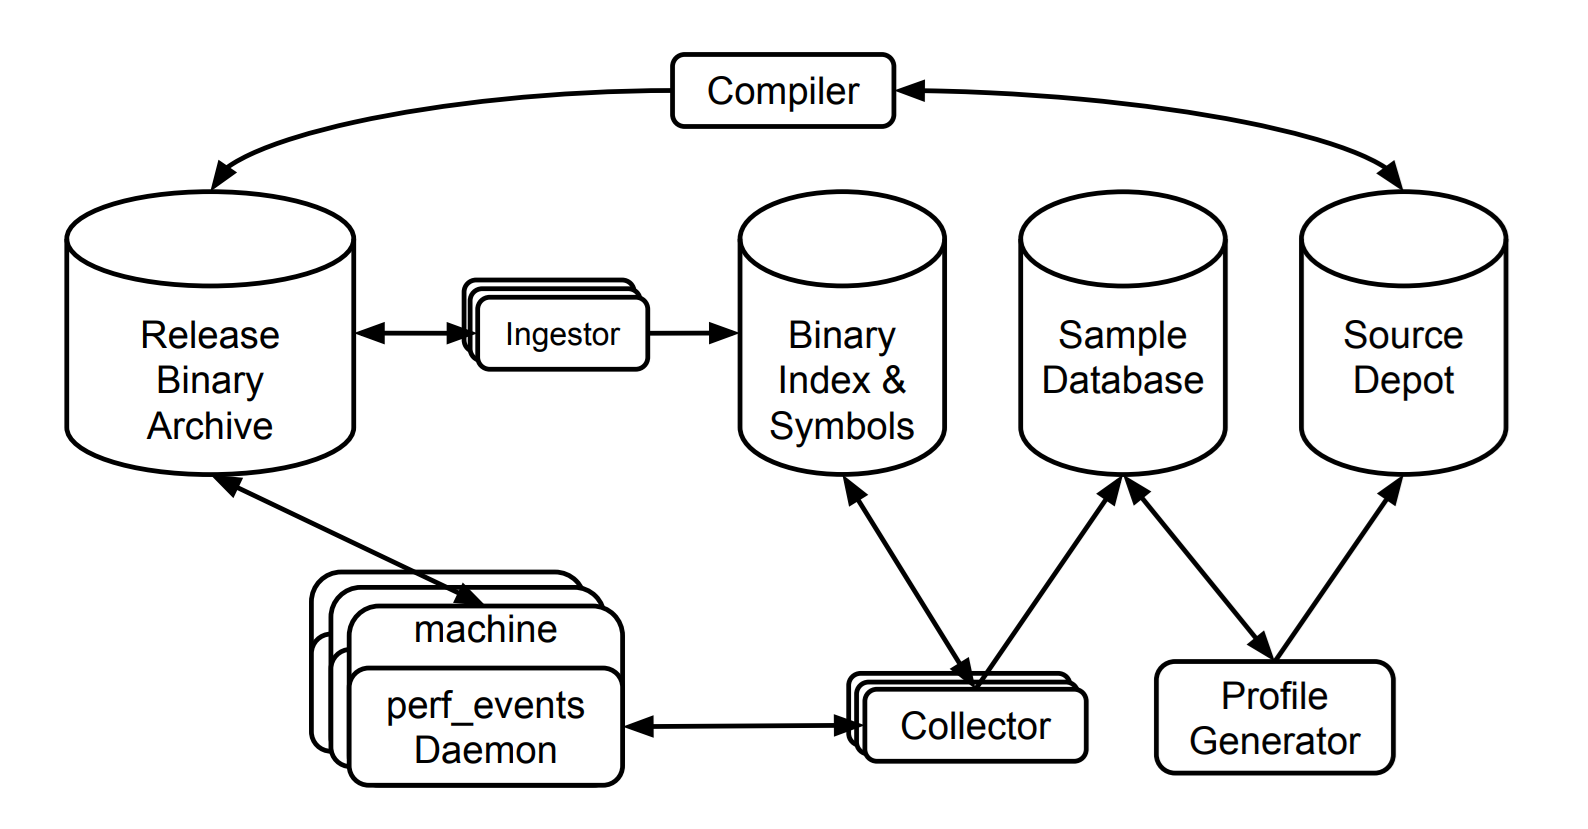
\includegraphics[scale=0.4]{PNG/FDO2}
	}
	\caption{Схема системы автоматического сбора профиля и рекомпиляции. \cite{chen2016autofdo}.}\label{partReview:fdo2}
\end{figure}

Сергей Лисицын  в своей диссертации \cite{SergeyL1} предлагает разрешить проблему зависимости профиля от входных данных с помощью версионирования отдельных участков программы, выбор между которыми делается динамически во время исполнения. Из минусов подобного решения можно отметить увеличение размеров исполняемого файла.

С популяризацией машинного обучения появилась возможность генерации качественного синтетического профиля \cite{rotem2021profile}. Авторы статьи натренировали бустинг над деревьями для генерации профильной информации, что в свою очередь позволило компилятору использовать этот профиль и применять соответствующие оптимизации. С помощью данного подхода авторам удалось добиться ускорения в 1.6 процента в среднем с максимальным результатом в 16 \%  на интерпретаторе языка Python. 
 \begin{figure}[htbp]
	\centering
	\includesvg[width = 400pt, inkscapelatex=false ]{SVG/pgowithoutprofile.drawio.svg}
	\caption{Схема компиляции с искусственным профилем.}
	\label{partReview:pgo_without profile}
\end{figure}
На рисунке \ref{partReview:pgo_without profile}а изображена тренировка модели, которая заблаговременно проводится разработчиками компилятора, а на рисунке \ref{partReview:pgo_without profile}б изображен рабочий режим, в котором работает компилятор, оказавшись у пользователя.

\FloatBarrier

\chapter{Методология и окружение}\label{ch:chMethod}
Как упоминалось во Введении, для решения поставленной задачи - улучшения компилятора - необходимо определить неоптимальные места в коде, сгенерированным компилятором, которые при исполнении показывают недостаточную эффективность или вызывают задержку конвейера исполнения.

Во второй главе рассматривается методология поиска неоптимальностей в коде приложений и замера производительности. 

В разделе \ref{p1:platform} дается описание целевой платформы, под которую разрабатывались оптимизации.

В разделе  \ref{p1:tests} описаны два основных пакета приложений, на которых демонстрировались результаты разработанных методов.

В разделе \ref{p1:method} излагается методология получения результирующих цифр, основанная на многолетнем научном опыте.

В разделе \ref{p1:optop} приводятся основные методы изучений целевых приложений для последующей разработки компилятивных алгоритмов. Рассмотрены такие методы как профилирование, симуляция и обратная разработка.


\section{Целевая платформа}\label{p1:platform}

Для проведения исследований был выбран широко распространенный сервер компании Huawei - Kunpeng920. Он базируется на архитектуре ARM V8.2-A \cite{reid2016trustworthy,xia2021kunpeng}.  Основным конкурентом данного процессора на архитектуре ARM является Ampere Altra Server \cite{cha2021ampere}.  Исследуемая модель процессора создана по 7-нанометровой технологии и оснащена 64 ядрами с тактовой частотой 2.6 ГГц. Модель включает в себя  ряд аппаратных ускорителей, в том числе криптографии (MD5, HMAC, CMAC, AES, DES/3DES,  SHA1, SHA2) и  алгоритмов сжатия (GZIP, LZS, LZ4). 

Каждый чип состоит из двух вычислительных кристаллов (SCCL - Рисунок \ref{chip1})  и одного кристалл интерфейса (SICL - Рисунок \ref{chip2}). Кристалл интерфейса, соединенный через общую шину, содержит модуль ускорителя криптографии, интерфейсы ввода/вывода, PCIE и т.п. Каждый вычислительный кристалл содержит 8 кластеров центрального процессора (CCL). В свою очередь, кластер центрального процессора состоит из 4х вычислительных ядер, 4х блоков кэширования первого уровня (64К для данных и 64К для инструкций), 4х блоков кэшировния второго уровня и блока тэгов для кэша третьего уровня. Кэш третьего уровня располагается отдельно внутри вычислительного кристалла, присоединенный к общей шине, в нем также могут храниться данные из других вычислительных кристаллов. Каждое ядро представляет собой 4-х канальный суперскалярный модуль с возможностью нарушения порядка исполнения (superscalar, out-of-order).

Интересной особенностью исследуемого процессора является широкая кэш-линия третьего уровня. Она составляет 128 байт, что в два раза превосходит общепринятое на рынке значение в 64 байта. 

\begin{figure}[htbp]
	\centering
	\includesvg[width = 300pt, inkscapelatex=false ]{SVG/wikichip1.drawio.svg}
	\caption{Схема целевого чипа}
	\label{chip1}
\end{figure}
\begin{figure}[htbp]
	\centering
	\includesvg[width = 300pt, inkscapelatex=false ]{SVG/SICL.drawio.svg}
	\caption{SICL модуль.}
	\label{chip2}
\end{figure}

Поддерживаемые расширения:
\begin{itemize}
	\item  \textbf{NEON} - Векторное расширение ARMv8
	\item  \textbf{CRC32} - Расширение для быстрого подсчета чек-суммы CRC32
	\item  \textbf{Crypto} - Криптография
	\item  \textbf{FP16} - Числа с плавающей точкой половинной точности
	\item  \textbf{RAS} -  Надежность, доступность и удобство обслуживания. (Reliability, Availability, and Serviceability)
\end{itemize}

\section{Тесты производительности}\label{p1:tests}
\subsection{SpecCPU 2017}\label{p1:tests:spec}
В проведенном исследовании использовались два набора тестов: "SpecCPU 2017"\phantom{ } \cite{bucek2018spec} и CPUBench \cite{lu2023cpubench}. 

"SpecCPU 2017"\phantom{ } - набор тестов для оценки производительности вычислительных систем. Существует два поднабора: целочисленный и набор тестов с плавающей арифметикой. Большая часть текущего исследования сосредоточена на улучшение производительности тестов с целочисленной арифметикой, однако некоторые общие подходы также применимы и к программам, использующим вычисления с плавающей точкой. Считается, что набор тестов SpecCPU является представителем современного рынка вычислений, поэтому многие компании при покупке вычислительных систем сравнивают производительность с использованием именно этого набора тестов. \cite{bucek2018spec}

Набор приложений, входящих в пакет "SpecCPU int 2017":
\begin{itemize}
		\item  \textbf{perlbench}:  Интерпретатор языка Perl, из которого было удалено большинство особенностей, связанных с операционными системами. Включает в себя набор тестов, которые измеряют время выполнения различных операций в Perl \cite{siever1998perl}.
		\item  \textbf{gcc}: Известный компилятор языков С/C++/Fortran из коллекции компиляторов GNU \cite{gough2004introduction}. 
		\item  \textbf{mcf}: Моделирует задачу коммивояжера, где необходимо найти оптимальный маршрут для распространения товаров в различных городах, минимизируя расстояние и время пути \cite{lobel1999solving}.
		\item  \textbf{omnetpp}: OMNeT++ моделирует производительность  сети, используя алгоритмы и структуры данных для симуляции различных сценариев, таких как передача данных, маршрутизация и управление трафиком \cite{varga2019practical}.
		\item  \textbf{xalancbmk}: Моделирует производительность преобразования XML-документов в HTML- или другие XML-документы с использованием языка XSLT (XSL Transformations) \cite{euzenat2002xml}.
		\item  \textbf{x264}: Свободная и открытая библиотека для кодирования видео, которая обеспечивает высококачественное и быстрое кодирование видео в формате H.264 (MPEG-4 AVC) \cite{merritt2006x264}.
		\item  \textbf{deepsjeng}: Искусственный интеллект игры в шахматы, имеет больше 2600 ELO  \cite{sandin2021ssdf}.
		\item  \textbf{leela}: Алгоритм игры в GO, включающий оценку позиции на основе метода Монте-Карло, выборочный поиск по дереву на основе верхних доверительных границ и оценку хода на основе рейтингов ELO \cite{choi2022does} .
		\item  \textbf{exchange2}: Программа, разработанная для генерации нестандартных и сложных судоку. Использовался на неофициальных соревнованиях, которые могли длиться несколько дней \cite{10.1145/1124708.1124709}. 
		\item  \textbf{xz}: Содержит компрессионный и декомпрессионный алгоритмы \cite{koranne2011compression}. 
\end{itemize}

Набор приложений, входящих в пакет "SpecCPU fp 2017":
\begin{itemize}
	\item  \textbf{bwaves}:  Численное  моделирование взрывных волн. Первоначальная конфигурация задачи состоит из области высокого давления,  внутри которой находится небольшая область низкого давления. Сложная интерференционная  результирующая картина  решается при помощи уравнений Навье-Стокса \cite{auer1983intracranial}.
	\item  \textbf{cactuBSSN}: Моделирование черных дыр и гравитационных волн \cite{allen2007scientific}.
	\item  \textbf{namd}: Моделирование больших бимолекулярных систем. Почти все время выполнения тратится на расчет межатомных взаимодействий в небольшом наборе функций \cite{phillips2002namd}.
	\item  \textbf{parest}: Биомедицинская визуализация. Построение трехмерных моделей объектов из нескольких наблюдений на двумерной плоскости (например МРТ, КТ) \cite{hoon2007fully}.
	\item  \textbf{povray}: Алгоритм трассировки лучей \cite{plachetka1998pov}.
	\item  \textbf{lbm}: Метод решеточных уравнений Больцмана для моделирования трехмерных моделей несжимаемых жидкостей.
	\item  \textbf{wrf}: Модель предсказания погоды, написанная на языке FORTRAN. Содержит огромное количество линейного кода \cite{skamarock2019description}. 
 	\item  \textbf{blender}: Рендер трех-мерных моделей \cite{brito2007blender}. 
 	\item  \textbf{cam4}: Модель циркуляции атмосферы \cite{neale2013mean}. 
 	\item  \textbf{imagick}: Производит последовательные манипуляции с двухмерной картинкой (повороты, отражения, размытие и т.д.) \cite{still2006definitive}. 
 	\item  \textbf{nab}: Приложение молекулярного моделирования, выполняющее интенсивные вычисления с плавающей запятой, которые обычно встречаются в области медико-биологических наук \cite{povcanic2009nab}. 
 	\item  \textbf{fotonik3d}: Вычисляет коэффициент передачи фотонного волновода, используя метод конечных разностей во временной области для уравнений Максвелла \cite{sullivan2013electromagnetic}.
 	\item  \textbf{roms}: Региональная система моделирования океана. Используется для исследования реакции океана на локальные изменения, такие как ветер или изменение температуры \cite{haidvogel2008ocean}. 
\end{itemize}



В наборе тестов SpecCPU существует два основных типа замера - speed и rate. В режиме speed разрешается использовать оптимизации с профилем, опции для каждого теста могут подбираться индивидуально. Однако в данной диссертации используется режим rate, в котором набор опций для всех тестов должен быть унифицирован и использование профиля запрещено. Запуск возможен как в режиме  одной копии - ресурсы машины доступны одному процессу полностью, так и  в режиме множественности копий, в котором процессам приходится делить общие ресурсы, такие как шину памяти или кэши. Стоит отметить, что ни в каком из наборов нельзя использовать прямо или косвенно информацию, специфичную для конкретных тестов. Так, например, в 2024 году более 2000 результатов  были помечены, как использующие информацию о тестах, а значит нечестные \cite{cliffFlagged}.

\subsection{CPUBench}\label{p1:tests:cpubench}

В 2023 году Китайский институт электроники и стандартизации выпустил новый набор тестов производительности для вычислительных систем \cite{lu2023cpubench}. В отличие от набора SpecCPU, интерфейс CPUBench разработан на языке python, а сам пакет имеет в себе программы, написанные на языке java. Авторами утверждается, что данный набор тестов является своеобразным расширением SpecCPU 2017, которое нацелено на лучшее покрытие мирового рынка (в том числе китайского). Было продемонстрировано на 14 различных платформах, что данный набор тестов сохраняет корреляцию производительности, показываемую пакетом SpecCPU.

Целочисленный набор состоит из следующих тестов:
\begin{itemize}
	\item  \textbf{x264, gcc, xz}: Схожие с пакетом "SpecCPU int 2017", отличаются наборами входных данных и версиями приложений.
	\item  \textbf{gzip}: Архиватор, использующий алгоритм LZMA2 \cite{akoguz2016comparison}.
	\item  \textbf{tpcc}: Бенчмарк, который моделирует  деятельность розничного дистрибьютора с большим количеством складов и клиентов \cite{leutenegger1993modeling}.
	\item  \textbf{tpch}: Еще одна база данных, однако эта состоит набора бизнес-ориентированных запросов и модификаций данных. Иллюстрируется система принятия решений \cite{barata2015overview}.
	\item  \textbf{kmeans}: Java тест, решающий задачу K-ближайших соседей.
	\item  \textbf{wordcount}: Java тест, подсчитывающий количество слов в больших файлах. 
	\item  \textbf{velvet}: Пакет алгоритмов, разработанный для сборки генома и выравнивания секвенирования коротких считываний \cite{zerbino2008velvet}. 
	\item  \textbf{openssl}: Криптографический инструментарий, реализующий различные алгоритмы шифрования \cite{rescorla2001introduction}.
	\item  \textbf{rapidjson}: Библиотека для парсинга Json -файлов\cite{keiser2023demand}
	\item  \textbf{python}: Интерпретатор языка Python \cite{python2021python}.
\end{itemize}
Набор тестов с плавающей точкой представлен следующим набором:
\begin{itemize}
	\item  \textbf{lightgbm}: Библиотека градиентного бустинга для машинного обучения \cite{ke2017lightgbm}.
	\item  \textbf{nektar}: Высокопроизводительный масштабируемый решатель для широкого спектра уравнений в частных производных \cite{cantwell2015nektar++}.
	\item  \textbf{phenglei}: Программная платформа вычислительной гидродинамики, разработанная Китайским центром исследований и разработок аэродинамики \cite{zhao2020design}.
	\item  \textbf{phyml}: Программа анализа белков и генов с помощью алгоритма максимального правдоподобия \cite{guindon2010new}.
	\item  \textbf{gromacs}: Пакет используется для моделирования различных биомолекул, имеющих большое количество межатомных связей \cite{van2005gromacs}.
	\item  \textbf{povray}: Алгоритм трассировки лучей \cite{plachetka1998pov}.
	\item  \textbf{openfoam}: Моделирование задач механики сплошных сред \cite{jasak2009openfoam}. 
	\item  \textbf{lammps}: Расчеты классической молекулярной динамики, применяется на суперкомпьютерах, имеет высокую степень парализации \cite{gowthaman2023review}.
	\item  \textbf{cube}: Гравитационная задача N-тел \cite{yu2018cube}.
	\item  \textbf{wrf}: Модель предсказания погоды, написанная на языке FORTRAN. Содержит огромное количество линейного кода \cite{skamarock2019description}. 	        
\end{itemize}

Можно заметить некоторую схожесть пакета CPUBench int с пакетом "SpecCPU int". Так, вместо интерпретатора языка perl представлен интерпретатор более современного языка python, добавлен дополнительный алгоритм компрессии/декомпрессии, парсинг XML документов заменен на парсер JSON файлов. А вот алгоритмов искусственного интеллекта здесь не наблюдается, зато присутствую базы данных MySQL и криптографический инструмент openssl.

Что касается тестов с плавающей точкой, большинство представленных программ в SpecCPU можно разделить на 2 категории: работа с графическими объектами и научные вычисления, в то время как в пакете CPUBench из графических приложений можно увидеть только алгоритм трассировки лучей, однако CPUBench содержит в себе библиотеку градиентного бустинга lightgbm, активно применяющуюся в машинном обучении. 

\section{Методология измерения}\label{p1:method}
В данной диссертаций используется измерения типа  "SpecCPU rate" и ее аналог typcal в CPUBench. В данной методологии предусмотрены следующие шаги:
\begin{enumerate} 
		\item Измерение времени выполнения каждого теста, запущенного в $NUM\_COPIES$ копий, в некоторое количество итераций ($N$)
		\item Если было запущено больше одной копии, то временем исполнения теста считается самое большое время среди всех копий.
		\item Для каждого теста выбирается медианное время среди проделанных итераций. 
		\item Обратное медианное время каждого теста умножается на референсное время ($REF\_TIME$), полученное на фиксированной машине. Например, для "SpecCPU 2017"\phantom{ }это  Sun Fire V490 with 2100 MHz UltraSPARC-IV+.
		\item Считается среднее геометрическое по всем тестам. Использование среднего геометрического обосновывается свойством сохранения отношения.
		\item Полученное число умножается на количество копий.
\end{enumerate}
Если всего в сете $M$ тестов, то кратко можно записать формулу расчета производительности следующим образом:

$$RATE =\left(\prod _{i=1}^{M}\dfrac{REF\_TIME_i}{MEDIAN(TIME_{i1}, TIME_{i2}, ... , TIME_{iN})}\right)^{\frac {1}{M}} $$

Также важной частью считается настройка окружающей системы, направленная на уменьшение флуктуаций времени исполнения тестов и лучшей утилизации тестовой системы.
Эта тема не является прямой темой данного исследования, а лишь косвенного затрагивает ее, но тем не менее весьма важна,поэтому ниже предлагается ознакомится с проблемами, которыми пришлось столкнуться во  время проведения замеров для алгоритмов, реализованных в данной диссертации.  

\begin{itemize}
	\item  \textbf{Троттлинг}. Технология изменения частоты процессора при превышении критических температур. Часто возникает при нарушении системы охлаждения или неправильной эксплуатации. Проявляется в виде увеличения времени исполнения теста с каждой следующей итерацией \cite{zhang2009hardware}.
		\begin{figure}[ht]
		\centerfloat{
			\includegraphics[scale=1]{PNG/ddr1}
		}
		\caption{Схема подсистемы памяти целевой платформы.}\label{fig:ddrsvg1}
	\end{figure}
	\item  \textbf{Неполная утилизация ресурсов системы}. Целевая платформа имеет восемь каналов DRAM, с возможностью подключения до двух плашек на каждый канал (Рисунок \ref{fig:ddrsvg1}). В случае, если какой-то канал остался незадействованным (Например, вставлены подряд, а не через одну) то будет наблюдаться картина, как на рисунке \ref{fig:lack_of_memmory}. Можно видеть, что неиспользуемые порты приводят к тому, что вычислительным ядрам приходится обращаться за ресурсами памяти в соседние блоки, что значительно замедляет исполнение.

	
	\begin{figure}[ht]
		\centerfloat{
			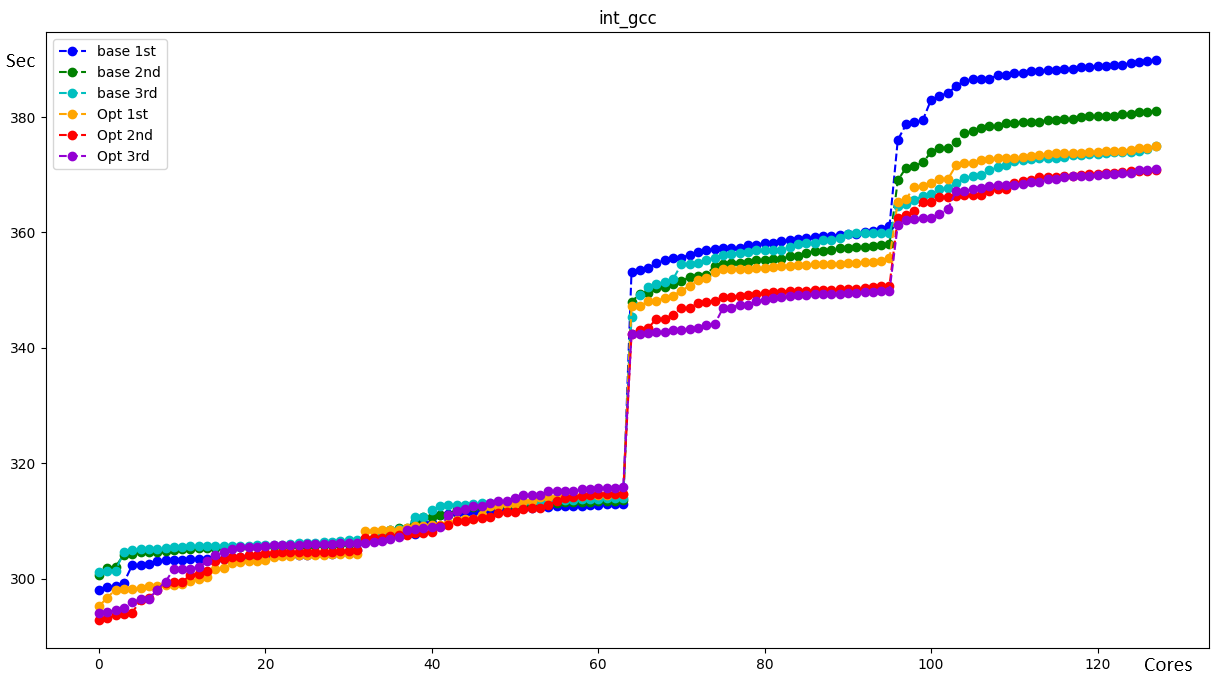
\includegraphics[scale=0.5]{PNG/lack_of_memmory}
		}
		\caption{Зависимость времени исполнения приложения от номера ядра при неправильном подключении плашек оперативной памяти.}\label{fig:lack_of_memmory}
	\end{figure}
	\item \textbf{Рандомизация размещения адресного пространства (ASLR)}. Технология, изначально разрабатываемая для защиты процессов от различного рода атак с использованием  переполнения буфера. При этом  адреса расположения исполняемого файла рандомизируются для усложнения предсказания положения объекта в памяти и получения доступа из сторонних процессов \cite{gras2017aslr}. Однако, в случае аккуратных измерений производительности системы эта технология может приводить к случайному наложению младших частей адресов и соответственно попаданию в одну и ту же кэш линию. На рисунке \ref{fig:peaks}  можно видеть как на случайном ядре время исполнения отдельной копии увеличивается больше, чем в 2 раза.
	\item \textbf{Частота обновления оперативной памяти} - Оперативная память, являясь энергозависимой памятью, требует постоянного обновления значений в ячейках. Частота обновления этих ячеек регулируется в BIOS. С одной стороны, большая частота обновления уменьшает количество ошибок и связанных с ними задержек, однако с другой стороны, обновление памяти это по своей сути дополнительная загрузка данных, что в высоко нагруженной системе может создавать дополнительные задержки. Поэтому этот параметр приходится подбирать эмпирическим путем, и он оказывает существенное влияние на итоговую производительность системы.
	
	\begin{figure}[ht]
		\centerfloat{
			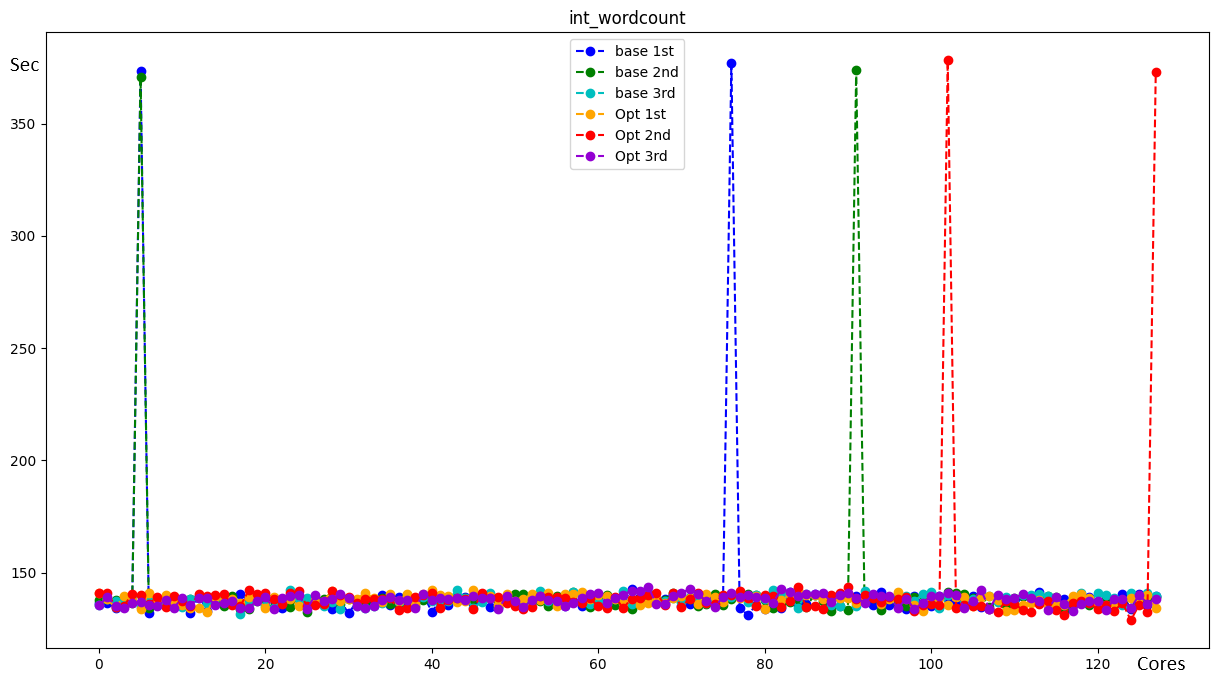
\includegraphics[scale=0.5]{PNG/peaks}
		}
		\caption{Зависимость времени исполнения приложения от номера ядра при замере c включенной ASLR.}\label{fig:peaks}
	\end{figure}
	\item \textbf{Занятость ресурсов внешними программами}. Достаточно очевидный факт: если необходимо измерить производительность системы, то ваш бенчамрк должен быть единственным, исполняемым на этой системе.  Однако, организовать тест в изоляции достаточно сложно, так как операционная система время от времени может запускать демонов, планировщик и прочее,  методы борьбы с этим индивидуальны и не будут указаны здесь, однако, покажем, как пронаблюдать этот эффект. Если мы производим высокоинтенсивной замер, утилизирующий все ядра и большинство остальных ресурсов системы, а затем отсортируем время выполнения тестов на разных ядрах, то можем получить картину, как на рисунке \ref{fig:tails}. Эти "хвосты"\  чаще всего означают, что система была занята другими  приложениями, а не  тестом.
\end{itemize}


\begin{figure}[ht]
	\centerfloat{
		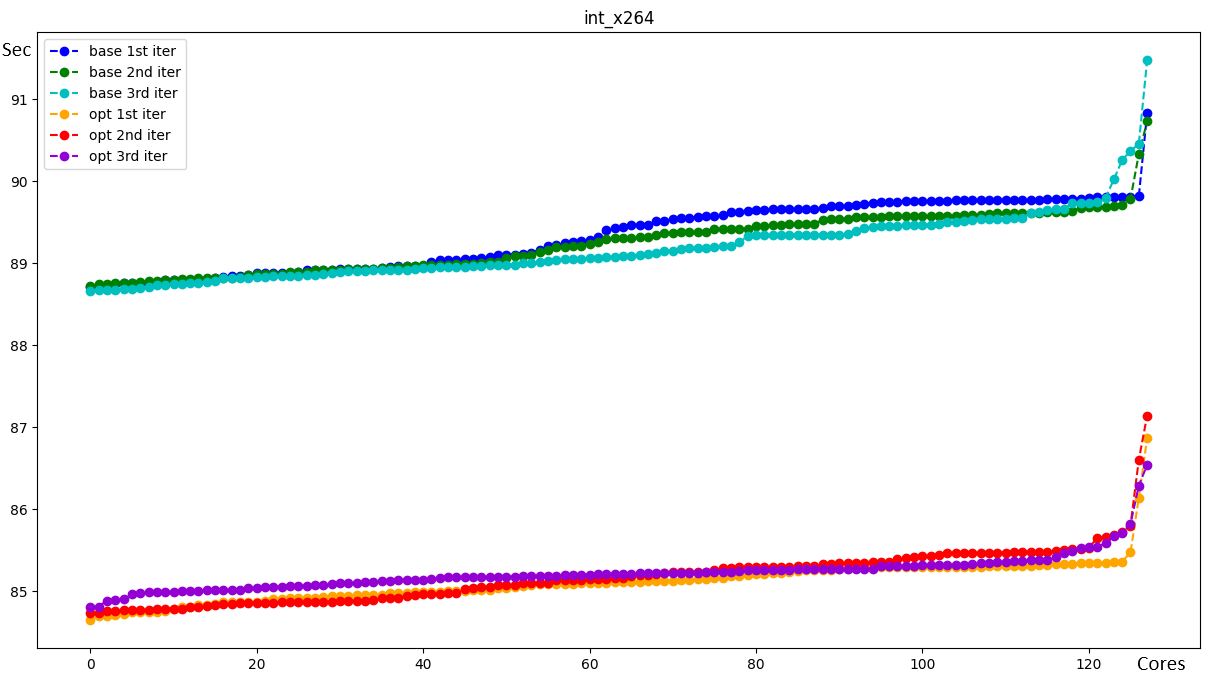
\includegraphics[scale=0.5]{PNG/tails}
	}
	\caption{Зависимость времени исполнения приложения от номера ядра при замере на загруженной системе.}\label{fig:tails}
\end{figure}



Приведенные проблемы нельзя решить после замера каким-либо "обрезанием хвостов"\  или "удалением пиков"\  из выборки. Методология такого не позволяет. Если бы подобные манипуляции были возможны, то это позволило бы вендорам манипулировать данными, ведь тогда пришлось бы вводить какие-либо правила, когда и как можно корректировать данные замеров, что привело бы к махинациям ради получения более высоких цифр производительности.

\section {Выявление возможностей для оптимизации}\label{p1:optop}
Данное исследование подразумевает выявление оптимизационных возможностей тестовых приложений для последующей разработки оптимизаций. К сожалению, очень сложно предоставить определенный алгоритм поиска оптимизационных возможностей, так как разные программы оказывают нагрузку разного типа на систему, подход к каждому случаю практически индивидуален, и должен учитывать аппаратные возможности, архитектуру команд и структуру исходной программы. Однако существуют достаточно понятные методологии поиска горячих (высоконагруженных) участков. Рассмотрим методы, которые использовались в данной диссертационной работе.

\subsection {Профилирование}\label{p1:optop:profile}
\textbf{Профилирование программы}  - это методика динамического анализа программы, которая способна измерить количество вызовов функций, загруженность памяти, использование определенных инструкций,  временную сложность программы.

Программы профилирования приложений в зависимости от способа сбора информации можно глобально разделить на три типа:

Первый тип профилирующих программ базируется на внутрипрограммных событиях. Для этого в код самого приложения или в код подгружаемых библиотек  вставляются дополнительные обработчики на этапе компиляции или линковки приложения. В процессе исполнения программа непосредственно перед заранее определенным программным событием (вызов функции, аллокация памяти, создание объекта и пр.) вызывается встроенным метод-обработчик, который собирает и агрегирует полезную профильную информацию. Классическим примером такого профилировщика является \textbf{gprof} \cite{graham2004gprof}. При таком способе внутрипрограмные события собирается с высокой точностью, однако постоянный запуск обработчиков может искажать перфомансную картину приложения (перебивать данные в кэшах и  влиять на логику предсказателей). Огромным минусом данной модели является необходимость перекомпиляции программы.

Другой подход - интерпретирующие профилировщики, по своей сути являющиеся бинарными трансляторами/интерпретаторами с возможностью выставления любых программных счетчиков непосредственно в код исполняемой программы во время исполнения \cite{reinders2005vtune, nethercote2007valgrind}. Являются мощнейшими инструментами профилирования, однако оказывают сильное влияние на время исполнение программы, замедляя ее в десятки или даже сотни раз. Тем не менее такой подход не требует перекомпиляции самого приложения и обладает высокой точностью сбора внутрипрограммных событий.

Третий подход и один из основных методов выявления оптимизационных возможностей в рамках данной диссертационной работы -  сэмплирующий профилировщик \textbf{perf} \cite{de2010new}. Он способен проверять стек вызовов программы через регулярные промежутки времени, благодаря интерфейсу прерываний операционной системы. Профили, собранные таким образом, обычно менее точны и не очень конкретны (могут пропускать вызовы функций), однако позволяют измеряемой программе работать практически на полной скорости. Относительная точность достигается путем агрегации большого количества данных. Такой тип профилирования наиболее удобен для больших приложений, используемых пользователями.


Важной особенностью сборки профильной информации является поддержка аппаратных счетчиков в архитектуре ARM64, реализованная в виде PMU (Performance Monitoring Unit). PMU это специализированный блок процессора, предназначенный для отслеживания различных событий, которые происходят на уровне микроархитектуры \cite{hansen2020examining}. PMU может быть управляем через специальные инструкции, такие как MCR (Move to Coprocessor from Register) и MRC (Move to Register from Coprocessor), позволяющие записывать и считывать данные из блока-монитора. Для контроля этого устройства существует 32 программируемых счетчика, которые могут быть настроены для отслеживания различных событий. Каждый счетчик может быть настроен для отслеживания конкретного события. В качестве примера событий, которые могут быть собраны благодаря PMU, можно привести:
\begin{itemize}
	\item Промахи в L1/L2/L3 кэш.
	\item Задержки в очереди на исполнение.
	\item Задержки, связанные с "голодом" исполняющих устройств (нет доступных для исполнения инструкций).
	\item Ошибки предсказания переходов.
	\item Задержки фронт-енда аппаратуры.
	\item Количество векторных инструкций.
	\item Количество инструкций с плавающей точкой. (метрика недоступна на исследуемой машине)
\end{itemize}


Такой метод позволяет очень сильно сузить круг поиска возможных оптимизаций. Так, например, в тестах xz и gzip наблюдалось значительное количество задержек в память, что в последующем послужило мотивацией к разработке дополнительных алгоритмов программной предподкачки данных. В тестах openssl, tpcc, tpch, python наблюдалось высокое количество задержек, связанных с фронт-ендом аппаратуры, частые ошибки предсказания переходов. В последующем этот анализ дал толчок к разработке оптимизации свертки условных переходов. Малое количество векторизованного кода в x264 привело к улучшению алгоритма векторизации.


\subsection {Симуляция}\label{p1:optop:sim}

Иногда общих соображений из главы \ref{p1:optop:profile} недостаточно для определения причин замедления программы. В таких случаях можно произвести исследование на потактововом симуляторе данной машины или близкой к ней по конфигурации и временным параметрам, при отсутствии точной модели. В качестве примера приведем пример анализа из оригинальной работы, посвященной оптимизации инструкций широкого доступа в память \cite{chernonog2024widemem}, позволившее реализовать оптимизацию \ref{ch2:split_ldp_stp}.

В качестве потактовой модели был использован симулятор GEM5, содержащий детальную модель микроархитектуры процессора Alpha 21264 \cite{lowe2020gem5,qiu2023performance}. Конфигурация симулируемой системы приведена в таблице \ref{tab:setupsim}. Важно подчеркнуть, что моделирование осуществляется в режиме эмуляции системных вызовов (system emulation), в котором отсутствует исполнение кода ядра операционной системы. 

\begin{table} [htbp]
	\centering
	\begin{threeparttable}% выравнивание подписи по границам таблицы
		\caption{Настройка симулируемой модели}\label{tab:setupsim}%
		\begin{tabular}{| m{5cm} | m{8cm}l |}
			\hline
			\hline
			\centering Архитектура			 & \centering  ARMv8.2-A & \\
			\hline
			\centering Модель процессора			 & \centering ArmO3CPU  & \\
			\hline
			\centering Кэш-память L1			 & \centering 64 кБ кэш данных, 64 кБ кэш инструкций  & \\
			\hline
			\centering Кэш-память L2			 & \centering 512 кБ, общий  & \\
			\hline
			\centering Ширина этапов конвейера			 & \centering 4 для всех этапов  & \\
			\hline
			\centering Количество LSU блоков & \centering 2   & \\
			\hline
			\centering Оперативная память 	& \centering  DDR4 2400 МГц 512 МБ  & \\
			\hline
			\hline
		\end{tabular}
	\end{threeparttable}
\end{table}


\begin{figure}[ht]
	\centerfloat{
		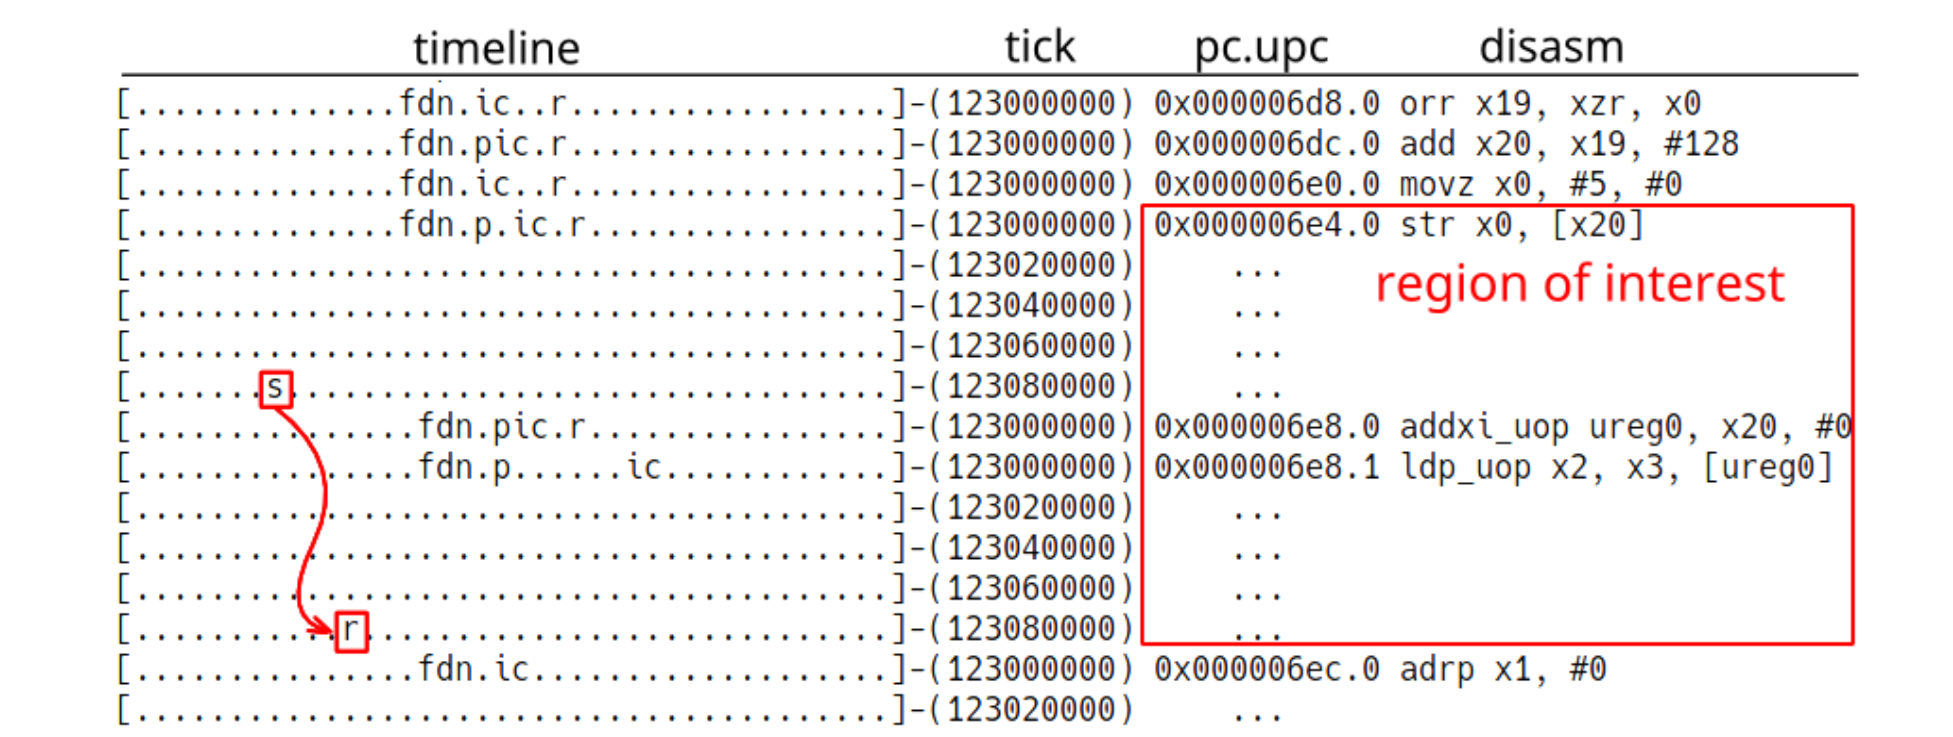
\includegraphics[scale=0.35]{PNG/simstep1}
	}
	\caption{Моделирование исполнения широкой инструкции чтения после записи.}\label{fig:simstep1}
\end{figure}
\begin{figure}[ht]
	\centerfloat{
		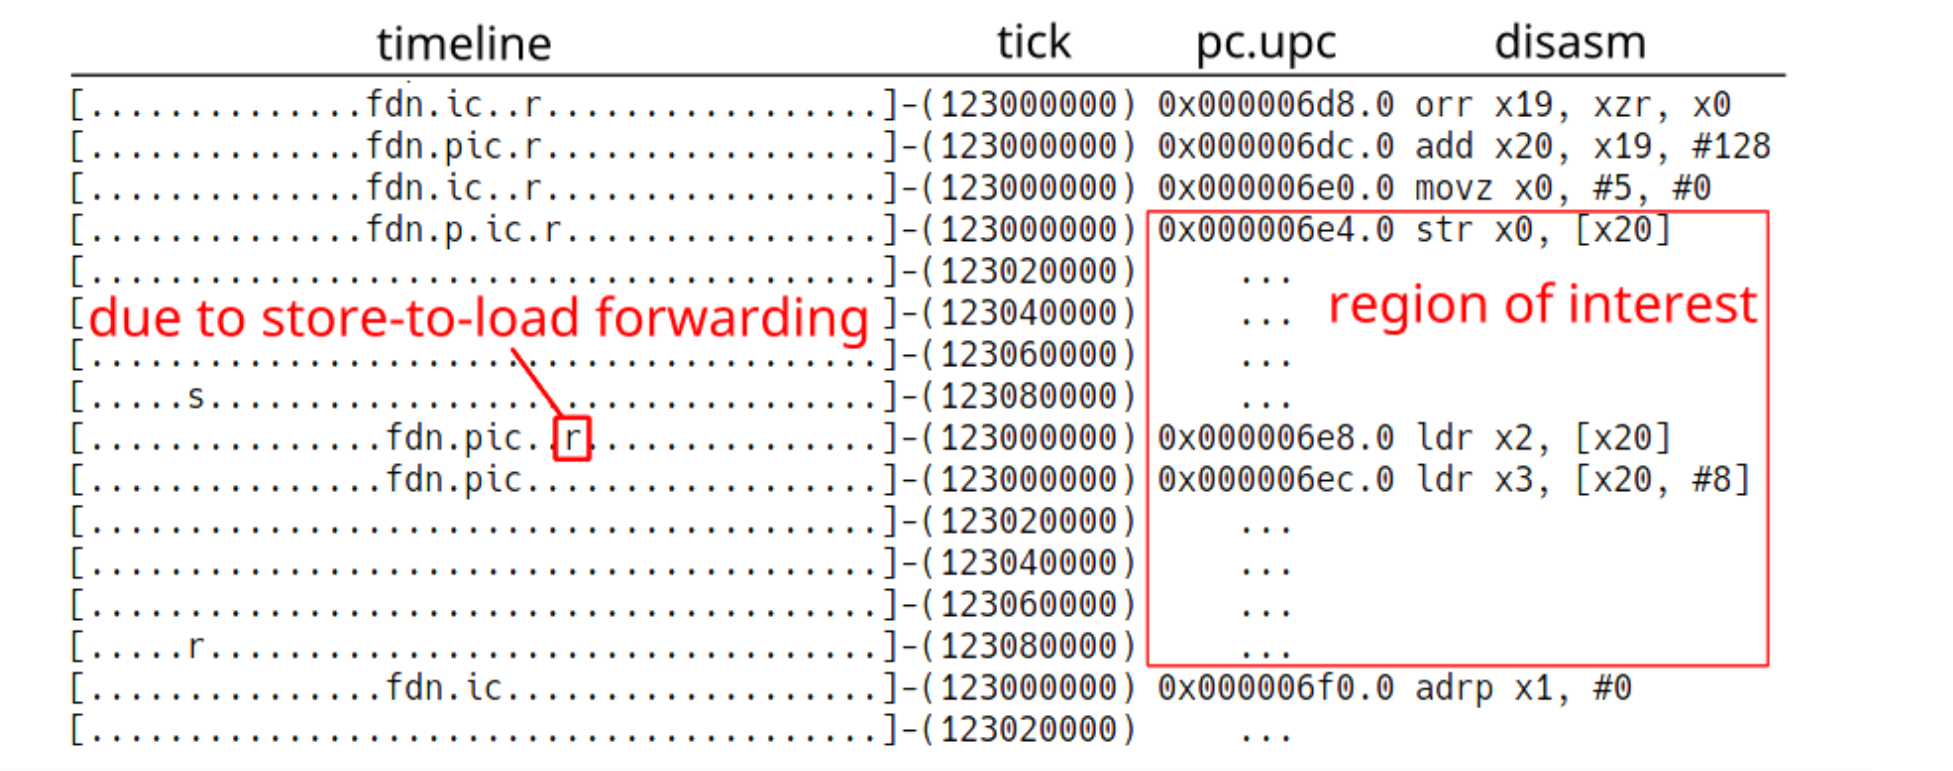
\includegraphics[scale=0.35]{PNG/simstep2}
	}
	\caption{Моделирование исполнения двух инструкций, полученных в результате разбиения широкой инструкции чтения памяти.}\label{fig:simstep2}
\end{figure}
\begin{figure}[ht]
	\centerfloat{
		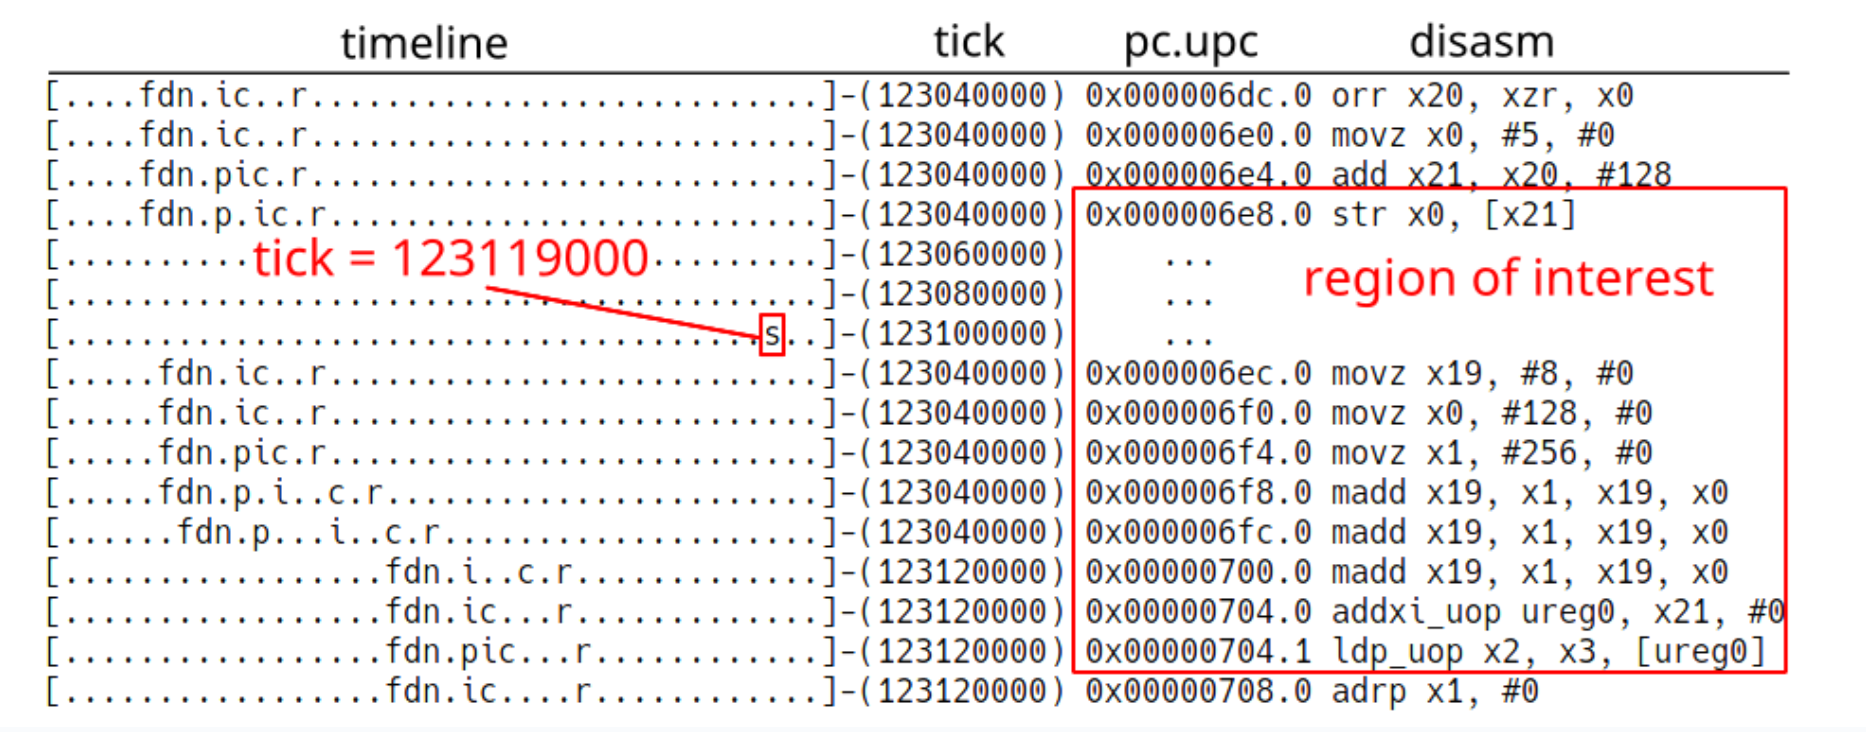
\includegraphics[scale=0.35]{PNG/simstep3}
	}
	\caption{Моделирование исполнения арифметических операций перед широкой инструкцией доступа в память.}\label{fig:simstep3}
\end{figure}
\begin{figure}[ht]
	\centerfloat{
		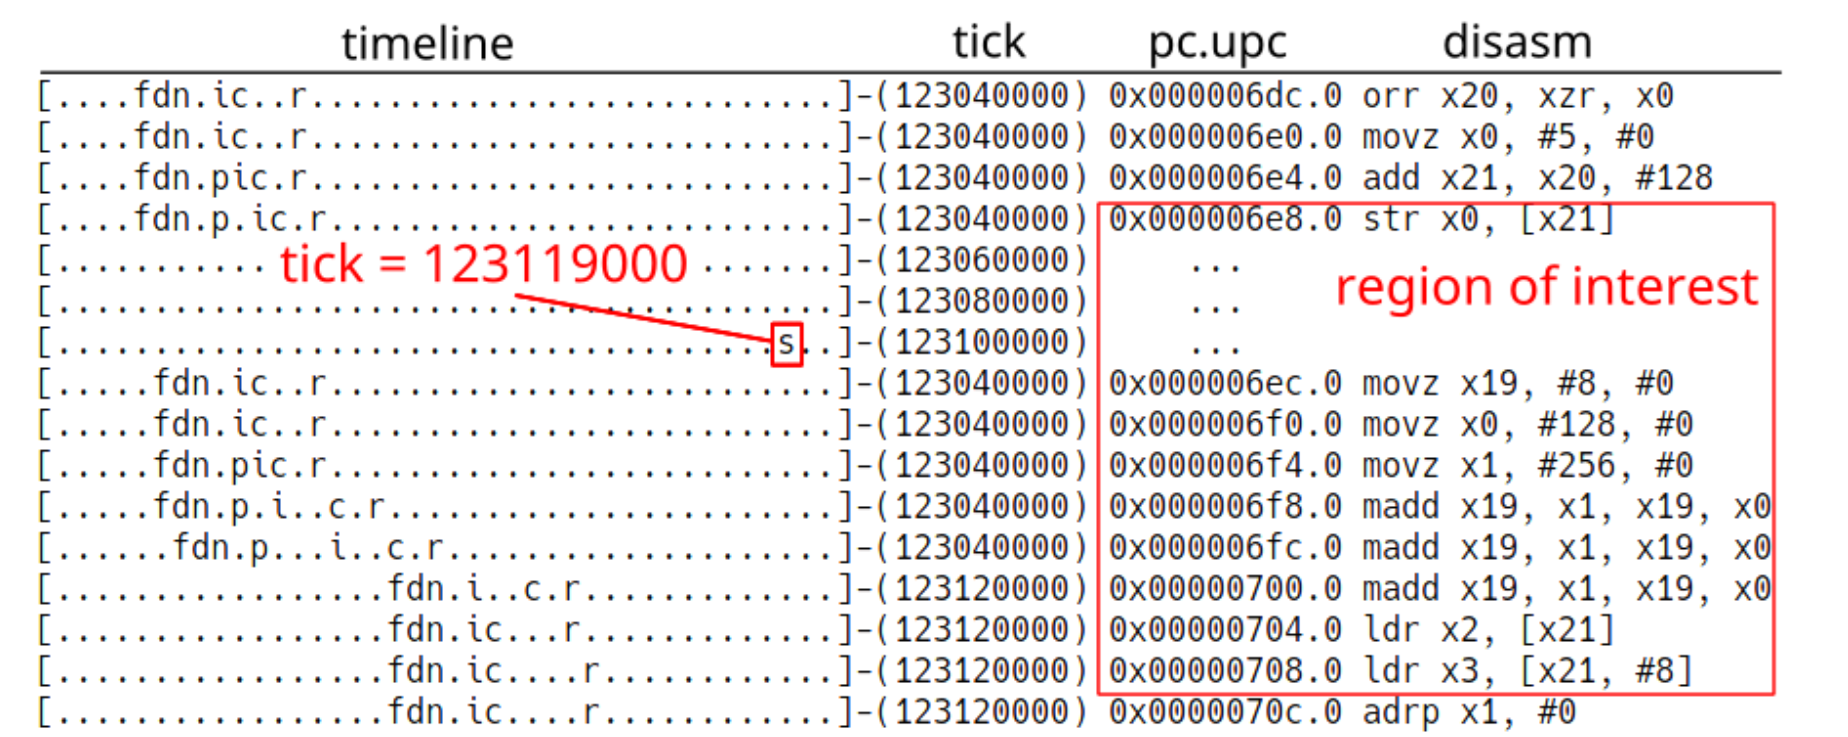
\includegraphics[scale=0.35]{PNG/simstep4}
	}
	\caption{Моделирование исполнения арифметических операций перед двумя инструкциями, полученными в результате разбиения широкой инструкции чтения .}\label{fig:simstep4}
\end{figure}

На рисунке \ref{fig:simstep1} приводится код, содержащий инструкции записи (STR) и  широкого чтения (LDP) с одинаковым базовым регистром. 
В левой части рисунка располагается временная шкала. Каждая точка соответствует одному циклу центрального процессора, там же указаны стадии конвейера:
\begin{enumerate}
\item f - fetch - чтение инструкции из ячейки памяти 
\item d - decode - разбор инструкции и ее аргументов
\item n - rename - переименование регистров (маппинг на физические)
\item p - dispatch - отправка инструкции в бек-енд (back-end) процессора
\item i - issue - назначение конкретного вычислительного устройства
\item c - complete - окончание исполнения
\item r - retire - возвращение результата операции пользователю
\item s - store-complete - завершение операции записи в память 
\end{enumerate}

В рассматриваемом сценарии процессором выполняется чтение, реализованное через инструкцию LDP, 16 байт данных, но перед чтением с помощью инструкции STR обновляются 8 байт в том же диапазоне памяти. Возникающий конфликт называется зависимостью "чтение после записи". Видно, что разбитая на микрооперации инструкция LDP переходит на этап r (retire) только спустя 4 такта после завершения записи в память.





На рисунке \ref{fig:simstep2} проиллюстрирована работа  аппаратного механизма разрешения зависимостей при спекулятивном выполнении операций доступа в память. Видно, что задержки не происходит.

Между рассматриваемыми инструкциями чтения и записи процессором могут выполняться прочие операции, и к моменту начала исполнения операции чтения запись в память полностью завершится. Моделирование такой ситуации для двух ранее рассмотренных случаев продемонстрировано на рисунках \ref{fig:simstep3} и \ref{fig:simstep4}. В обоих случаях на чтение пары значений тратится одинаковое время, так как в очереди на запись уже нет данных, которые можно взять для первой инструкции чтения. Следовательно, разделение инструкции широкого доступа не всегда целесообразно и требует анализа. В общем случае максимальное число инструкций между двумя конфликтующими операциями доступа в память, которое далее будем называть дистанцией, зависит от конфигурации конкретного процессора и времени выполнения инструкций различного типа, поэтому предлагается определять это значение эмпирическим путем.

\subsection{Обратная разработка}\label{p1:optop:reverse}

Чаще всего под обратной разработкой понимают исследование некоторого готового продукта с целью изучения его свойств. Конечно же в проделанной работе тоже имелся такой этап. Для целевого оптимизатора конкурентами являются такие компиляторы как LLVM Clang \cite{lattner2008llvm} и intel DPC++ \cite{castano2022evaluation}. Обратная разработка позволяет провести быстрый визуальный анализ сгенерированного кода и, что самое важное,  модифицировать его без необходимости перекомпиляции. Среди существующих популярных инструментов дизассемблера (IDA, Radare2, Ghidra и др. \cite{ferguson2008reverse, mester2023malware, jiang2022comprehensive}) был выбран radare2. Его преимуществами являются четкое описание установки на своей странице Github, наличие обширной документации и поддержки сообщества на своей странице Wikipedia и своей официальной электронной книге.

\begin{figure}[htbp]
	\centering
	\includesvg[width = 500pt, inkscapelatex=false ]{SVG/gzip_longest_match.svg}
	\caption{Базовые блоки горячего участка кода приложения gzip, полученные с помощью radare2}
	\label{radare2}
\end{figure}

\section{Выводы по главе}

Во второй главе приводится описание целевой архитектуры,  методы исследования приложений и замера цифр производительности. 

Рассмотрены проблемы, связанные с процессом измерения цифр производительности, описаны их архитектурные причины.

На примерах исследуемых приложений показано использование программного обеспечения для анализа тестов на целевой архитектуре.




\chapter{Разработка оптимизаций}\label{ch:ch2}

В этой главе описаны разработанные оптимизации. Не все представленные оптимизации были приняты сообществом openEulerGCC \footnote{https://gitee.com/src-openeuler/gcc/} по разным причинам. Некоторые из описанных далее оптимизаций будут представлены сообществу позднее, а некоторые, возможно, будут заменены другими подходами. Тем не менее автор считает, что исследованные подходы также представляют научный интерес.


\section{Улучшение существующих оптимизаций}\label{sec:ch2/sect1}
Хотелось бы начать описание проделанной работы с улучшений уже существующих оптимизаций. Компилятор GCC разрабатывается c 1987 года. Сотни разработчиков и исследователей привносили  свои улучшения все это время, тем не менее в процессе данной работы с учетом специфики целевой машины удалось найти определенное количество недостатков даже в существующих алгоритмах.
 
\subsection{Преобразование условных переходов} \label{opt:ifconv}
Преобразование условных переходов (If-conversion) — это хорошо известный метод оптимизации, который заменяет инструкцию перехода и зависящий от него поток управления предикатным исполнением, соединяя тем самым две различные ветки потока управления в одну для последующего совместного исполнения.  В результате целевой код содержит меньшее количество инструкций перехода, что снижает нагрузку на аппаратный предсказатель переходов, однако такой подход позволяет увеличить количество избыточных инструкций во время исполнения \cite{bruel2021if,E240105}. Обычно эта оптимизация основана на представлении SSA, однако в компиляторе GCC используется другой подход. На этом этапе SSA форма отсутствует, что может привести к следующей проблеме (рис. \ref{fig:ifcvtsvg1}): если в одной из ветвей исполнения в качестве регистра назначения используется  тот же регистр (reg1 на
Рисунке \ref{fig:ifcvtsvg1}), что в другом в качестве источника, то после слияния будет создано неправильное определение reg1.

Предлагаемое решение содержит принудительное переименование регистров. Такая трансформация была добавлена при коллизии такого типа. Регистры коллизий определяются как:

$$rename\_candidates = DEFS_{left\_bb} \cap USES_{right\_bb} $$
Если $rename\_candidates[i]$ все еще жив в конце базового блока $BB$, то трансформация не может быть применена.


\begin{figure}[htbp]
	\centering

	\includesvg[width = 400pt, inkscapelatex=false ]{SVG/ifcvt-1.svg}
	\caption{Пример некорректного преобразования условных переходов в следствие отсутствия SSA формы}
	\label{fig:ifcvtsvg1}
\end{figure}

Улучшение преобразования условных переходов в компиляторе GCC было размещено под опцией \mbox{\textbf{-fifcvt-allow-register-renaming}}. Такой подход помогает уменьшить количество "хвостовых"\   базовых блоков в целевых тестах. (Листинг \ref{ifcvtcode1}). Такие базовые блоки были обнаружены путем применения технологии профилирования из главы \ref{p1:optop:profile}. Сбор событий при помощи PMU показывал повышенное количество задержек во фортн-энде (front-end) процессора. Причиной этих задержек оказались постоянный переходы в "хвостовые"\   базовые блоки и обратно.


\begin{ListingEnv}[!h]
	\captiondelim{ } % разделитель идентификатора с номером от наименования
		\caption{Пример "хвостовых"\  базовых блоков, которые будут оптимизированы предложенным улучшением преобразования условных переходов}
	\label{ifcvtcode1}
	\begin{Verb}
		4145bc:   ret
		4145c0:   mov     x5, #0x100000000              
		4145c4:   add     x7, x7, x5
		4145c8:   b       4131d0
		4145cc:   mov     x2, #0x100000000               
		4145d0:   add     x6, x6, x2
		4145d4:   b       4145a0 
		4145d8:   mov     x3, #0x100000000                
		4145dc:   add     x11, x11, x3
		4145e0:   b       41454c
		4145e4:   mov     x3, #0x100000000 
		4145e8:   add     x11, x11, x3
		4145ec:   b       4144fc 
	\end{Verb}
\end{ListingEnv}

Конечно же применение подобной трансформации сопряжено с определенными рисками уменьшения производительности. Повсеместное преобразование может привести к увеличенному давлению на регистровый файл, что в свою очередь приводит к излишнему использованию стека. Поэтому вводятся функции стоимости для данной оптимизации: главным, однако далеко не единственным критерием применения преобразования условных переходов является итоговый размер базового блока, в  разработанной модели, этот параметр может задаваться пользователем, однако на исследуемой машине эмпирически был выведен  ограничивающий размер  результирующего базового блока равный 48 инструкциям.
\begin{ListingEnv}[!h]
	\captiondelim{ } % разделитель идентификатора с номером от наименования
	\caption{Образец проверки из теста povray (трассировка лучей)}
	\label{ifcvtcode2}
	\begin{Verb}
		if (lf == 0.0 || lf * f < 0)
		{
			changes++;
		} 
	\end{Verb}
\end{ListingEnv}


\begin{ListingEnv}[!h]
	\captiondelim{ } % разделитель идентификатора с номером от наименования
	\caption{Листинг \ref{ifcvtcode2} в представлении GIMPLE GCC}
	\label{ifcvtcode3}
	\begin{Verb}
		<bb 9> [local count: 118111600]:
		if (lf_11 == 0.0)
		goto <bb 11>; [50.00%]
		else
		goto <bb 10>; [50.00%]
		
		<bb 10> [local count: 59055800]:
		_5 = lf_11 * val_42;
		if (_5 < 0.0)
		goto <bb 11>; [41.00%]
		else
		goto <bb 12>; [59.00%]
		
		<bb 11> [local count: 83268678]:
		changes_22 = changes_10 + 1;
		
		<bb 12> [local count: 118111600]:
		# changes_9 = PHI <changes_10(10), changes_22(11)>
	\end{Verb}
\end{ListingEnv}
В качестве примера дополнительных ограничений рассмотрим оптимизацию участка кода из теста povray (трассировка лучей). В одном из основных горячих циклов можно встретить следующую проверку, изображенную на листинге \ref{ifcvtcode2}. В GCC этот код трансформируется в следующий набор базовых блоков (Листниг \ref{ifcvtcode3}) Операция умножения считается достаточно тяжелой, поэтому преобразование ее в  один базовый блок вместе с простым сравнением с нулем кажется компилятору неэффективным, однако было обнаружено, что для конкретной исследуемой платформы такое преобразование все же увеличивает итоговую производительность программы.  



\begin{ListingEnv}[!h]
	\captiondelim{ } % разделитель идентификатора с номером от наименования
	\caption{Листинг \ref{ifcvtcode3} в представлении GIMPLE GCC после оптимизации преобразования условных переходов}
	\label{ifcvtcode4}
	\begin{Verb}
		<bb 9> [local count: 118111600]:
		_5 = lf_11 * val_42;
		_36 = _5 < 0.0;
		_51 = lf_11 == 0.0;
		_18 = _36 | _51;
		if (_18 != 0)
		goto <bb 10>; [70.50%]
		else
		goto <bb 11>; [29.50%]
		
		<bb 10> [local count: 83268678]:
		changes_22 = changes_10 + 1;
		
		<bb 11> [local count: 118111600]:
		# changes_9 = PHI <changes_10(9), changes_22(10)>
	\end{Verb}
\end{ListingEnv}

Оптимизация реализована в проходе ifcombine на этапе  Gimple. Следующее преобразование было введено для оптимизации целевого кода  и оно основано на том факте, что некоторые инструкции быстрее (или дешевле с точки зрения времени), чем условные переходы (рисунок \ref{ifcvt2svg1}). Это означает, что объединение двух сравнений в рамках операции AND или OR в один базовый блок, чтобы не выполнять "ленивое"\phantom{} вычисление булевого оператора, является более эффективным. Реализация gcc по умолчанию объединяет текущее сравнение со следующим, только если оно является условным. Эта оптимизация определяет список дешевых gimple-assign-insns, которые также могут быть объединены в один базовый блок в этом проходе.

\begin{figure}[htbp]
	\centering
	\includesvg[width = 400pt, inkscapelatex=false ]{SVG/ifcvt2.drawio.svg}
	\caption{Схема улучшения стоимостной эвристики в оптимизации преобразования условных переходов}
	\label{ifcvt2svg1}
\end{figure}

Введение дешевых инструкций и добавление туда умножения чисел с плавающей точкой позволяет в примере из листинга \ref{ifcvtcode3} объединить  базовый блок, содержащий сравнение float var с 0.0, c блоком с дешевой инструкцией умножения с плавающей точкой.Таким образом, один условный оператор goto и один базовый блок будут удалены. После этого преобразования оптимизированный фрагмент будет выглядеть следующим образом во внутреннем представлении компилятора GCC (Листинг \ref{ifcvtcode4}).

\subsection {Векторизация циклов с небольшим числом итераций}
Векторизация — это известный метод, использующий параллелизм данных \cite{nuzman2006autovectorization}. В ходе текущего исследования было обнаружено, что векторизация генерирует "хвосты"\phantom{ }(т. е. векторизованный код для меньшего коэффициента векторизации), но не использует их, когда фактическое количество итераций равно коэффициенту векторизации хвоста ($VEC\_FACTOR$). Опять же, чтобы это увидеть пришлось воспользоваться техникой сэмплирующего профилирования из главы \ref{p1:optop:profile}, в ходе которой было обнаружено, что несмотря на включенную векторизацию, приложение все равно большую часть времени исполняла скалярную версию участка. Следовательно, когда $VEC\_FACTOR$ равен, например 8, код будет сгенерирован для $VEC\_FACTOR = 4$ и $VEC\_FACTOR = 2$. Если во время выполнения фактическое количество итераций будет только 4, то будет выбран скалярный вариант. Это небольшое и простое улучшение меняет условие пересечения указателя в заголовке цикла \cite{E240105}.

Рассмотрим простой цикл (Листинг \ref{algexample_1})

\begin{ListingEnv}[!h]
	\captiondelim{ } % разделитель идентификатора с номером от наименования
	\caption{Простой цикл рассматриваемый оптимизацией векторизации}\label{algexample_1}
	\begin{Verb}
		\\ a,b,c: any arrays with size N
		for (i = 0; i<N; i+=1)
		    c[i] = a[i] *b[i]
	\end{Verb}
\end{ListingEnv}
GCC преобразует этот цикл в (Листинг \ref{vectorized_loop_example}), и легко видеть, что если, например, $c-a = VEC\_FACTOR/2$ и $N = VEC\_FACTOR/2$, то будет выбрана скалярная версия.

\begin{ListingEnv}[!h]
	\captiondelim{ } % разделитель идентификатора с номером от наименования
	\caption{Цикл (Листинг \ref{algexample_1}) после векторизации GCC}\label{vectorized_loop_example}

	\begin{Verb}

		\\ a,b,c: any arrays with size N
		VEC_FACTOR: factor estimated by GCC pass
		if  (abs (c - a) < VEC_FACTOR  ||  
		     abs (c - b) < VEC_FACTOR) 
		    goto SCALAR;

		if (N < VEC_FACTOR)
		    goto TAIL;
			
		for (i;i<N;i+=VEC_FACTOR)
		    WIDE_C = WIDE_A * WIDE_B 
		    \\ WIDE_X has VEC_FACTOR size 
			
		TAIL:
		if (i<N - VEC_FACTOR/2)
		    goto SCALAR;
			
		SEMIWIDE_C = SEMIWIDE_A * SEMIWIDE_B 
		\\ SEMIWIDE has VEC_FACTOR/2 size 
		
		SCALAR:
		for (i = 0; i<N; i+=1)
		    c[i] = a[i] *b[i]

	\end{Verb}
\end{ListingEnv}

\begin{ListingEnv}[!h]
	\captiondelim{ } % разделитель идентификатора с номером от наименования
	\caption{Модифицированная проверка для (Листинг \ref{vectorized_loop_example})}\label{replaced_check}
	
	\begin{Verb}
		
		
		\\ a,b,c: any arrays with size N
		\\ VEC_FACTOR: factor estimated by GCC pass
		if (abs (c - a) < min(VEC_FACTOR,N) ||
		    abs (c - b) < min(VEC_FACTOR,N)) 
		   goto SCALAR;
	\end{Verb}
\end{ListingEnv} 

Чтобы это исправить, предлагается простое решение: заменить строки 1 и 2 в векторизованной версии (Листинг \ref{vectorized_loop_example}) следующим кодом (Листинг \ref{replaced_check}). Добавлен параметр \textbf{--param=vect-alias-flexible-segment-len}. Эта оптимизация повышает производительность приложения x264.

\subsection {Векторизация линейного кода}

Векторизация линейного кода (SLP - superword level parallelism) \cite{rosen2007loop,guo2017new} является одной из известных проблем в области оптимизирующих компиляторов.  В процессе исследования было обнаружено, что современный компилятор GCC не может векторизовать код, представленный на листинге Листинге \ref{cube_base_vec}.  Данный горячий участок кода содержит последовательность из четырех групп инструкций: по 2  выгрузки и 2 загрузки в память. 

\begin{ListingEnv}[!h]
	\captiondelim{ } % разделитель идентификатора с номером от наименования
	\caption{Пример кода для векторизации из теста cube}\label{cube_base_vec}
	
	\begin{Verb}
		rho_f[idx1[2]][idx1[1]][idx1[0]] +=
			dx1[0] * dx1[1] * dx1[2] * sim.mass_p_cdm;
		rho_f[idx1[2]][idx1[1]][idx2[0]] +=
			dx2[0] * dx1[1] * dx1[2] * sim.mass_p_cdm;
		rho_f[idx1[2]][idx2[1]][idx1[0]] +=
			dx1[0] * dx2[1] * dx1[2] * sim.mass_p_cdm;
		rho_f[idx1[2]][idx2[1]][idx2[0]] +=
			dx2[0] * dx2[1] * dx1[2] * sim.mass_p_cdm;
		rho_f[idx2[2]][idx1[1]][idx1[0]] +=
			dx1[0] * dx1[1] * dx2[2] * sim.mass_p_cdm;
		rho_f[idx2[2]][idx1[1]][idx2[0]] +=
			dx2[0] * dx1[1] * dx2[2] * sim.mass_p_cdm;
		rho_f[idx2[2]][idx2[1]][idx1[0]] +=
			dx1[0] * dx2[1] * dx2[2] * sim.mass_p_cdm;
		rho_f[idx2[2]][idx2[1]][idx2[0]] +=
			dx2[0] * dx2[1] * dx2[2] * sim.mass_p_cdm;
		
	\end{Verb}
\end{ListingEnv}



В качестве улучшения оптимизации  векторизации линейного участка кода были предложены следующие шаги:
\begin{itemize}
	\item \textbf{Группировка инструкций}: Векторизация поддерживает группировку инструкций, адресующих не непрерывный участок памяти. В данном случае проход пытался собрать группы по 8 инструкций, после чего не мог векторизовать сложный набор. Было решено ограничить размер группы размером реального  векторного регистра на целевой машине.  Такое небольшое изменение позволило существенно упростить дальнейший анализ прохода, так как теперь в горячем участке формируются четыре группы, по 2 загрузки и выгрузки в каждой.
	\item \textbf{Анализ пересечения адресов}: Доступы в память не могут быть векторизованы, если не доказано, что они адресуют непересекающиеся ячейки памяти. Текущая реализация GCC обращает внимание только на базовые адреса инструкций. Например, загрузки
	$$LDR\phantom{S}R_1, R_b, 1$$
	$$LDR\phantom{S}R_2, R_b, 2$$
	считаются непересекающимися, так как имеют общую базу и разное смещение. Однако, если вторую инструкцию заменить на последовательность
	$$ADD\phantom{S}R_3, R_b, 1$$
	$$LDR\phantom{S}R_2, R_3, 1$$,
	то анализатор видит различные базовые регистры и не может определить пересечение. Данная проблема была решена добавлением аффинного анализа выражений в проход. С его помощью $R_3$ раскрывается как $1*R_b + 1$, и , если вычесть из этого многочлена $R_b$, то результатом будет константа.
	\item \textbf{Перестановка инструкций}: Наивная группировка инструкций приводит к тому, что группа выражений из листинга \ref{cube_base_vec2} формирует два вектора \{\_35,\_33\} и \{\_147,\_35\}, однако в таком случае чаще лучше бы было сгруппировать их иначе: \{\_35,\_35\} и \{\_147,\_35\}. Новая группировка позволит использовать аппаратное умножение вектора на скаляр, что ускоряет итоговые вычисления, за счет экономии процесса сборки лишнего вектора.
	\begin{ListingEnv}[!h]
		\captiondelim{ } % разделитель идентификатора с номером от наименования
		\caption{Выражения без перестановок}\label{cube_base_vec2}
		
		\begin{Verb}
				stmt 0: _61 = _35* _147
				stmt 1: _66 = _33 * _35
		\end{Verb}
	\end{ListingEnv}
\end{itemize}

Все эти изменения позволили векторизовать исходный участок из целевого теста cube (листинг \ref{cube_base_vec}), а также улучшить векторизацию линейных участков в компиляторе GCC.


\section{Шаблонные оптимизации}\label{sec:ch2/sect2}
Данный раздел поднимает вопрос шаблонных оптимизаций. Несмотря на свою кажущуюся простоту, этот тип оптимизаций позволяет поднять две важные проблемы. Первая  проблема это извечная борьба CISC и RISC подходов к разработке программного обеспечения. За усложнением архитектуры процессора следует усложнение работы транслятора. Другая поднимаемая проблема это современная популяризация различного рода ускорителей (криптография, матричное умножение, архивация и тд.). Дело в том, что ускорители подразумевают загрузку целых алгоритмов в них для исполнения, однако написание кода под этот ускоритель становится отдельной задачей для разработчиков программного обеспечения. В такой парадигме хотелось бы переложить работу поиска алгоритмов на компилятор, чтобы пользователю не приходилось реализовывать множество версий своего алгоритма для каждой платформы. 
\subsection{Оптимизация двойного умножения}
Оптимизация двойного умножения — это шаблонное преобразование компилятора, предназначенное для преобразования алгоритма 64-битного умножения в  эффективные инструкции. Таким образом, программа может лучше использовать возможности аппаратуры и повысить производительность всего приложения. Это стандартная архитектурно-зависимая оптимизация. Различные архитектуры предоставляют разные наборы команд. Иногда инструкции системы команд просты, что позволяет легко найти аналоги для любой архитектуры (например, инструкция add), но иногда, особенно в CISC-архитектурах, могут встречаться достаточно сложные инструкции, эквивалент которых потребует десятков и даже сотен команд.  \cite{bansal2021reduced, isen2009tale}.


Идея таких вычислений основана на максимальных значениях половинного умножения ($s$ - размер в битах).
\begin{equation*} \label{eq1}
	\left(2^{s/2}-1\right)^2=2^s-2^{s/2+1}+1<2^s-1
\end{equation*}

При разделении аргументов на части $s/2$ широкое умножение можно переписать как:
\begin{equation*} \label{eq2}
	\begin{split}
		res& =a\cdot b =\left(2^{s/2}a_{hi}+a_{lo}\right)\left(2^{s/2}b_{hi}+b_{lo}\right) \\
		& =2^sa_{hi}b_{hi}+2^{s/2}\left(a_{hi}b_{lo}+a_{lo}b_{hi}\right)+a_{lo}b_{lo}  
	\end{split}
\end{equation*}
Результат состоит из двух частей: младшей (от $1$ до $2^s - 1$) и старшей (от $2^s$ до $2^{2s} -1$). Первое слагаемое  и правая часть второго слагаемого станут старшей частью результата. левая часть второго и третьего слагаемых станут младшей частью результата.


\begin{equation*} \label{eq3}
	\begin{split}
		2^s\le2^sa_{hi}b_{hi}<2^{2s}
	\end{split}
\end{equation*}
\begin{equation*} \label{eq4}
	\begin{split}
		2^{s/2}& \le2^{s/2}\left(a_{hi}b_{lo}+a_{lo}b_{hi}\right)\\ 
		& \le2^{3s/2}\left(2^{s+1}-2^{s/2+2}+1\right)
	\end{split}
\end{equation*}
\begin{equation*} \label{eq5}
	\begin{split}
		1\le a_{lo}b_{lo}<2^s
	\end{split}
\end{equation*}
Несложно доказать, что сложения могут привести к переполнению во время этих вычислений. Переименуем слагаемые для лучшего восприятия:
\begin{equation*} \label{eq6}
	\begin{split}
		mid\_res&=a_{hi}b_{lo}+a_{lo}b_{hi} \\
		&=mid\_res\_real+mid\_res\_overflow
	\end{split}
\end{equation*}
\begin{equation*} \label{eq7}
	\begin{split}
		res_{lo}&=2^{s/2}mid\_res\_real_{lo}+a_{lo}b_{lo} \\
		&=res\_low\_real+res\_low\_overflow
	\end{split}
\end{equation*}

\begin{flalign*}  \label{eq8}
	res_{hi}&=middle\_res\_real_{hi}+a_{hi}b_{hi} \notag  \\
	&=res\_high\_real+\dfrac{res\_low\_overflow}{2^s}\\
	&\phantom{=res\_high\_real}+\dfrac{mid\_res\_overflow}{2^{s/2}} \notag 
\end{flalign*}



\begin{equation*} \label{eq9}
	res=2^s \cdot res_{hi}+res_{lo}
\end{equation*}

 Такие вычисления отыскиваются с использованием существующего механизма поиска шаблонов GCC и преобразуются в одиночные умножения более широких типов.  Количество инструкций значительно уменьшено. На CPUBench наблюдалось улучшение производительности в 30 \% на тесте OpenSSL.

\subsection{Шаблонная криптография}
В этом разделе поднимается важная тема для различных встраиваемых устройств и расширений архитектуры. В современном мире существует множество специализированных устройств для конкретных задач; например, ускорители для нейронных сетей \cite{chen2020survey}, для научных вычислений \cite{weber2010comparing}, для обработки графов \cite{rahman2020graphpulse} и т. д.

В недавнем исследовании \cite{peccerillo2022survey} Pecceriilo et al., 2022, классифицировали около 100 различных типов
ускорителей. Таким образом, в этой тенденции компилятор становится очень практичным инструментом, который может компилировать (потенциально автоматически) и планировать выполнение задач на разных устройствах. В настоящее время разные компании пытаются разработать собственный подход к решению этой задачи \cite{tavarageri2019automatic,chen2022case,kovac2022towards}.

Небольшая часть этой глобальной проблемы была решена в ходе нынешнего исследования. Kunpeng 920 имеет на плате расширение криптографии, которое включает специальные инструкции для crc32 и AES. Их можно использовать напрямую через встроенный язык ассемблера или встроенные функции компилятора. Добавлены оптимизации компилятора, которые могут определять возможность использования инструкций в соответствии с семантикой кода.

Оптимизация соотносит весь алгоритмам, включая предварительно рассчитанные таблицы, и статически проверяет, что все предварительно рассчитанные таблицы не изменяются во время выполнения. Оптимизация контролируется флагами \textbf{-fcrypto-accel-aes} и \textbf{-fcrypto-accel-crc32}. Оба шаблона были реализованы внутри RTL, поскольку они являются  архитектурно-зависимыми. На верхнем уровне логика оптимизаций очень похожа друг на друга. Следующие шаги описывают преобразование шаблона AES:

\begin{enumerate}
	\item \textbf{Сбор ссылок на таблицы AES}: Разработан оптимизационных проход внутри компилятора GCC для поиска ссылки на соответствующие таблицы шифрования/дешифрования AES. Такие инструкции являются отправной точкой для дальнейшего анализа.
	\item \textbf{Формирование раундов AES}: Анализируются ссылки на таблицы и собираются инструкции, выполняющие вычисления, относящиеся к AES. связывая их вместе в блоки и раунды.
	\item \textbf{Проверка шаблона AES}: Анализируются раунды и связываются вместе.
	\item \textbf{Генерация кода AES}: Генерируется код AES для всех найденных раундов.
\end{enumerate}

Для сопоставления внутреннего представления компилятора на уровне RTL использовался собственные шаблонный анализатор.Механизм сопоставления был создан на основе существующих генераторов сопоставлений match.pd GENERIC и GIMPLE.  Код для необходимой проверки шаблона генерируется во время компиляции GCC. Анализатор генерирует заранее упорядоченную последовательность аргументов.


Специальные инструкции сократили общее количество инструкций в целевых горячих циклах, что привело к значительному ускорению. Улучшение производительности на 10+ \% было достигнуто на
тестах openSSL и gzip.

К сожалению, оптимизация crc32 не была принята, поскольку менее общая оптимизация, обеспечивающая большую производительность при использовании gzip, была предложена другими авторами.

\subsection{Шаблонная подстановка инструкций}

Одной из основных основных задачей компилятора является выбор наиболее подходящих инструкций, которыми можно будет лаконично и в то же время оптимально с точки зрения производительности выразить внутреннее представление программы \cite{blindell2016instruction}. В данной работе  не изменяется работа стандартного прохода выбора инструкций, однако добавляется несколько небольших шаблонов, который способствуют лучшей утилизации набора команд архитектуры ARM64.

Так, арифметическое выражение вида 
\begin{flalign*}  \label{eq10}
	B = (((A &>> 15) \& 0x00010001) << 16) -\\
	((A &>> 15) \& 0x00010001)
\end{flalign*}

до внесенных изменений транслировалось в векторной версии в (Листинг \ref{unoptimal1}) может быть транслировано в (Листинг  \ref{optimal1})
\begin{ListingEnv}[!h]
	\captiondelim{ } % разделитель идентификатора с номером от наименования
	\caption{Пример неоптимального выбора инструкций №1}\label{unoptimal1}
	
	\begin{Verb}
			xtn v18.4h, v17.4s
			xtn2 v18.8h, v1.4
	\end{Verb}
\end{ListingEnv} 
\begin{ListingEnv}[!h]
	\captiondelim{ } % разделитель идентификатора с номером от наименования
	\caption{Оптимальный выбор инструкций для Листинга \ref{unoptimal1} }\label{optimal1}
	\begin{Verb}
			uzp1 v17.8h, v18.8h, v17.8h
	\end{Verb}
\end{ListingEnv} 

Таким  же методом был преобразован код  (Листинг \ref{unoptimal2}) в более оптимальную версию, использующую инструкции smin/smax на (Листинг \ref{optimal2})
\begin{ListingEnv}[!h]
	\captiondelim{ } % разделитель идентификатора с номером от наименования
	\caption{Пример не оптимального выбора инструкций №2 }\label{unoptimal2}
	\begin{Verb}
			sshr v1.4s, v1.4s, #10
			neg v24.4s, v1.4s
			mov v20.16b, v1.16b
			sshr v24.4s, v24.4s, #31
			bic v20.4s, #0xff
			cmeq v20.4s, v20.4s, #0
			bif v1.16b, v24.16b, v20.16b
	\end{Verb}
\end{ListingEnv} 
\begin{ListingEnv}[!h]
	\captiondelim{ } % разделитель идентификатора с номером от наименования
	\caption{Оптимальный выбор инструкций для Листинга \ref{unoptimal2} }\label{optimal2}
	\begin{Verb}
		movi v2.2d, #0x0 // (outside the loop)
		movi v3.2d, #0xff000000ff // (outside the loop)
		...
		smax v18.4s, v18.4s, v2.4s // (inside the loop)
		smin v18.4s, v18.4s, v3.4s // (inside the loop)
		uzp1 v17.8h, v18.8h, v17.8h
	\end{Verb}
\end{ListingEnv} 



\section {Девиртуализация} \label{opt:devirt}
 Высокоуровневые языки программирования, такие как Java, C++ и C\# и др. применяют динамические таблицы вызовов для реализации парадигмы полиморфизма\cite{calder1994quantifying,suganuma2000overview,bauer2021novt}.  В такой модели адрес вызываемой функции становится известным только во время исполнения программы. Виртуальные функции в объектно-ориентированных языках являются одним из основных источников косвенных переходов в программном коде. В языках C/C++ также можно использовать указатели на функции, а в GCC  существует отдельное расширение, которое позволяет пользователю брать адрес на метку в коде программы \cite{shah1995function}, что  позволяет пользователям создавать косвенные вызовы и переходы самостоятельно. 
 
 Несмотря на удобства во время написания программы, реализация переходов через косвенность  может замедлить работу центрального процессора, так как для эффективной обработки управляющих инструкций суперскалярному процессору необходимо предсказывать целевой адрес перехода. Для этого используются специальные устройства-предсказатели \cite{mcfarling1993combining,mittal2019survey}. Однако, реализация предсказателя косвенных переходов существенно разнится от предсказателя условных. В случае условного перехода существуют всего два конечных адреса передачи управления, но для косвенных переходов это не так, в следствие этого предсказателю приходится запоминать адреса перехода, что может существенно увеличить площадь, занимаемую предсказателем \cite{driesen1998accurate}. В литературе описывается принцип виртуального счетчика инструкций, однако это все еще требует дополнительной логики в аппаратуре \cite{redmond2007vpc}.
 Современные решения этой задачи в основном сосредоточены на разрешении вызовов виртуальных функций в контексте объектно-ориентированного программирования. Недостаток информации о целевых функциях в графе вызова затрудняет межпроцедурные оптимизации и делает невозможной подстановку функций непосредственно в код, что значительно ограничивает возможности компилятора для оптимизации \cite{li2010lightweight,pande1996data}.



В статье \cite{chernonog2023статический} описывается два метода преобразования косвенных переходов: статический и динамический.  

Статический метод по своей сути является расширением стандартной методологии девиртуализации компилятора GCC. Его работа разделена на две части:

\begin{enumerate}
	\item \textbf{Анализ сигнатур функций}: Авторами предлагается анализировать сигнатуры функций для определений и вызовов. Если сигнатура вызываемой функции совпадает с сигнатурой определения то функция определения считается кандидатом.
	\item \textbf{Трансформация косвенного перехода}: На этом этапе, в случае единственного кандидата, косвенный вызов функции заменяется вызовом найденной процедуры. Если же кандидатов несколько, то приходится выстраивать цепочку сравнений адресов переходов. что не всегда является оптимальным
\end{enumerate}


\begin{figure}[ht]
	\centerfloat{
		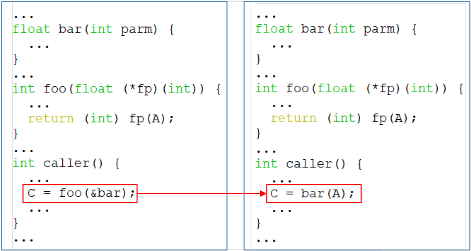
\includegraphics[scale=1]{PNG/ICP}
	}
	\caption{Пример замены косвенного вызова}\label{fig:ICP1}
\end{figure}

С другой стороны динамический метод использует информацию, собранную во время выполнения программы \cite{baev2015profile,ishizaki2000study}, чтобы изменить косвенные переходы. При этом повторная компиляция программы не происходит. В этом состоит отличие от методов, использующих профилирование или системы JIT-компиляции (Just-in-Time compilation). 
Для решения этой задачи предлагается внедрять инструменты для трансформации кода непосредственно в исполняемую программу. В системах JIT перекомпилированный код отдельного метода или функции обычно размещается в новом участке памяти \cite{cravvford1988study}. Однако здесь предлагается добавить буферный участок кода, который будет изменяться во время работы приложения.
 

\textbf{Алгоритм}
 \begin{enumerate}
 	\item \textbf{Выбор косвенных переходов}: Может происходить автоматически при помощи транслятора, на основе графа вызовов функций, либо в ручном. В поставляемой библиотеке доступны два макроопределения "DDL\_GOTO"\  и "DDL\_CALL", при мпомощи которых можно заменить переход goto или косвенный вызов функции на библиотечный примитив. 
 	\item \textbf{Трансформация косвенных переходов}: Вместо каждой инструкции перехода генерируется "окно"\  в виде заранее определенного количества NOP инструкций и вызовов библиотечных функций сбора статистики и замены инструкций nop условными переходами при превышении счетчиков. Оригинальный косвенный переход сохраняется в самом конце.
 	\item \textbf{Запуск программы и сбор статистики}: Этот этап и все последующие происходят во время выполнения программы и не требуют никаких действий от пользователя или компилятора. Каждый раз, когда программа достигает изменённого косвенного перехода, вызывается библиотечная функция для обновления статистики целевых адресов этого перехода. Библиотека собирает статистику отдельно для каждого перехода, который идентифицируется уникальным номером, присвоенным при инициализации.
 	
 	\item \textbf{Трансформация в реальном времени}: Когда накоплено достаточное количество статистических данных, заданное параметром N, запускается функция модификации кода программы. Целевые адреса сортируются по убыванию числа переходов к ним. Если 95 \% переходов осуществляется не более чем по k адресам, происходит замена последовательности инструкций NOP на условные переходы (листинг \ref{indirect_algo1}). В противном случае происходит вставка исходного косвенного перехода.
	\item \textbf{Работа оптимизированного перехода}: После изменения перехода сбор статистики целевых адресов прекращается. Тем не менее, информация о количестве выполнений этого перехода продолжает накапливаться, а также фиксируется число случаев, когда в преобразованном коде отсутствует прямой переход к полученному целевому адресу, что означает, что оптимизация для этого адреса не была выполнена и должен сработать первоначальный косвенный переход (расположенный дальше по коду). Если количество пропущенных переходов станет значительным по сравнению с общим числом входов в данный участок кода, цепочка прямых условных переходов будет заменена исходным блоком NOP инструкций, и сбор статистики возобновится. Иными словами, процесс вернется к шагу 2. При этом статистика адресов, собранная на предыдущем этапе выполнения шага 3, будет учитываться с коэффициентом 0.5, что позволит сохранить эту информацию.
 \end{enumerate}

\begin{ListingEnv}[!h]
	\captiondelim{ } % разделитель идентификатора с номером от наименования
	\caption{Псевдокод преобразованного косвенного перехода}\label{indirect_algo1}
	
	\begin{Verb}
		
		INT entry_count = 0;
		entry_count++;
		START_REWRITE_POINT:
		NOP
		NOP
		...
		NOP // k-times reapeat
		BOOL collect_stat_mode = FALSE;
		INT miss_count = 0;
		miss_count++;
		if ( entry_count == N)
		&& (miss_count > entry_count >> 4) {
			if (!collect_stat_mode){
				collect_stat_mode = TRUE;
				CALL DDL_DISABLE_OPTIMIZATON();
			} else {
				miss_count = 0;
				entry_count = 1;
				CALL DDL_REWRITE_INDIRECT();
				collect_stat_mode = FALSE;
			}
		}
		if (collect_stat_mode) {
			CALL DDL_UPATE_STATISTICS();
		}
		goto *addr; // original indirect branch
		
	\end{Verb}
\end{ListingEnv} 


\begin{ListingEnv}[!h]
	\captiondelim{ } % разделитель идентификатора с номером от наименования
	\caption{Пример преобразованного на ходу косвенного перехода}\label{indirect_algo2}
	
	\begin{Verb}
		
			mov       w9 #0xe20
			movk      w9 #0x40, lsl #16
			cmp       x28, x9
			b.eq      0x400e20
			movk      w9, #0xe60
			cmp       x28, x9
			b.eq      0x400e60
			movk      w9, #0xe30
			cmp       x28, x9
			b.eq      0x400e30
			movk      w9, #0xe40
			cmp       x28, x9
			b.eq      0x400e40
			movk      w9, #0xe50
			cmp       x28, x9
			b.eq      0x400e50
			movk      w9, #0xdd4
			cmp       x28, x9
			b.eq      0x400dd4
			movk      w9, #0xe10
			cmp       x28, x9
			b.eq      0x400e10
			nop
			nop
			...
	\end{Verb}
\end{ListingEnv} 

Статический подход способствовал улучшению тестов tpcc и tpch. Хотелось бы отметить, что улучшение openssl в статье \cite{chernonog2023статический} ошибочно и является следствием некачественной валидации бенчмарка openssl в пакете CPUBench, а также со стороны авторов.

Динамический подход не показал эффективности на всем тестовом пакете, однако на небольших мотивационных тестах  наблюдается улучшение производительности до 200 \%, когда количество адресов перехода находится в диапазоне от 4 до 8, в иных случаях может наблюдаться деградация. Деградация в 10 \% также наблюдалась на отдельных тестах пакета "SpecCPU 2017"\phantom{}.

\begin{figure}[ht]
	\centerfloat{
		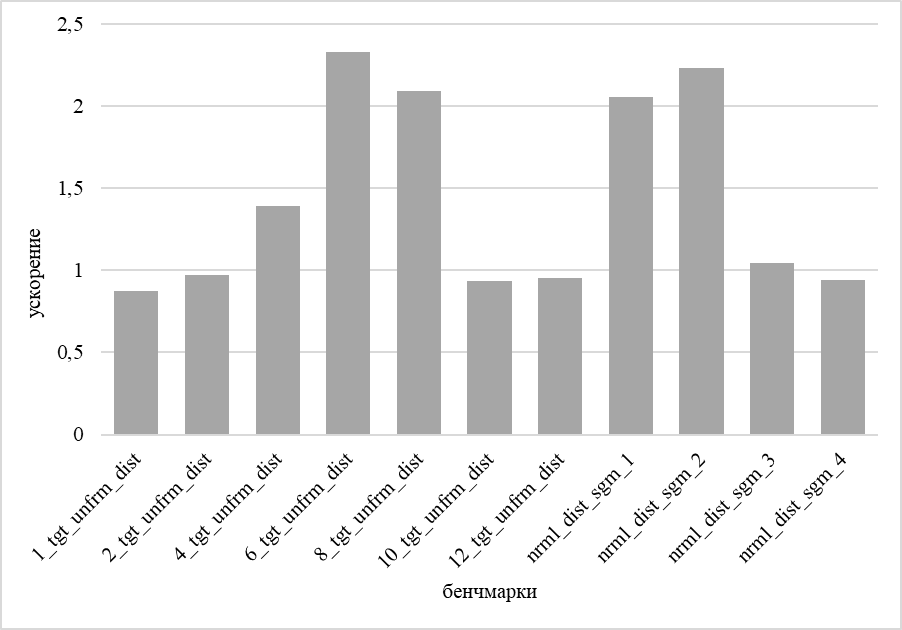
\includegraphics[scale=0.6]{PNG/ICP2}
	}
	\caption{Результаты замеров производительности динамического подхода в зависимости от распределения количества целевых адресов}\label{fig:ICP2}
\end{figure}


 \section {Разбиение широких инструкций доступа в память} \label{ch2:split_ldp_stp}
Архитектура ARM имеет сложные инструкции, которые выполняют содержат внутри себя несколько простых, например, арифметических или логических операций. Такие инструкции позволяют эффективно использовать ресурсы ЦПУ и уменьшают размер кода. Они повышают производительность и сокращают задержку выполнения операций. Однако для использования сложных инструкций необходимо тщательно понимать их функциональность и ограничения, чтобы обеспечить более качественное выполнение программы. Предыдущие исследования \cite{park2019microarchitecture} показали, что разделение 128-битных инструкций чтения из памяти  может улучшить производительность на отдельных тестах. В ходе данного исследования была продолжена эта работа, и было обнаружено, что в двух случаях использование широкого доступа может возникнуть потеря производительность.

\begin{figure}[htbp]
	\centering
	\includesvg[width = 400pt, inkscapelatex=false ]{SVG/split_ldr.drawio.svg}
	\caption{Два случая, когда использование широкого доступа в память приводит к замедлению}
	\label{splitsvg1}
\end{figure}

Один из них (см. рисунок \ref{splitsvg1}) - это хорошо известный "невыровненный доступ". Было выявлено, что широкий доступ к памяти должен бытькратен его формату, в противном случае производительность снижается (даже когда речь идет о загрузке 2х независимых регистров). С другой стороны, было показано, что Kunpeng 920 не может быстро обрабатывать зависимости чтения после загрузки в память, если они имеют разные размеры. Аппаратная оптимизация пересылки сохраняемого значения (store-to-load forwarding) \cite{shen2013modern} не может быть выполнена в таком случае. Подробный разбор данной ситуации на симуляторе целевой микроархитектуры можно увидеть в главе \ref{p1:optop:sim}. Поэтому было решено разделить широкие доступы к памяти в эмпирически установленном диапазоне.



\begin{figure}[htbp]
	\centering
	\includesvg[width = 300pt, inkscapelatex=false ]{SVG/wide_ldr.svg}
	\caption{Схема алгоритма разделения сложных инструкций}
	\label{splitsvg2}
\end{figure}

Для решения этой проблемы был разработан алгоритм (см. рисунок \ref{splitsvg2}), который находит инструкцию определения для базового регистра адреса широкой загрузки. Затем алгоритм ищет все использования этого определения, кроме оригинального. Если алгоритм находит сохранение в память с той же базой, то проверяется целесообразность разделения исходного широкого доступа к памяти. Было выявлено, что такой подход разумен, если расстояние между загрузкой и сохранением составляет менее 16 инструкций.

 \section {Уменьшение размеров типов переменных}
 Анализ диапазона значений переменных в компиляторе \cite{harrison1977compiler,  simon2008value}  может помочь в удалении избыточных условий, улучшении постоянного распространения, удалении избыточных вычислений и т. д. В результате исследования было выявлено, что анализ диапазона значений GCC все еще имеет недостатки. Прежде всего, текущая оптимизация распространение диапазона значений не способна получать диапазоны из неизменяемых структур данных, что может быть полезно для предварительно вычисленных таблиц. Кроме того, GCC не может изменить размер переменной. Например, если диапазон переменной - $\{0, 1\}$, но пользователь использует тип \textbf{int} для нее, это неоднозначно, для этого можно использовать тип \textbf{boolean}, то же самое касается \textbf{int64\_t} и \textbf{int32\_t}. К сожалению, это не относится к переменным с плавающей точкой, потому что точность может быть потеряна. Производительность на тесте gzip была улучшена.
 
 \section {Векторизация "ленивых"\phantom{ } вычислений}\label{ch2:lcv}
 "Ленивые"\phantom{ } вычисления в языках С/C++ являются частью стандарта языка. Такой подход помогает оптимизировать программы в том смысле, что необходимые вычисления производятся только в тот момент, когда они нужны, а не заранее \cite{cukic2018functional}. Например, в строке (if (pointer \&\& pointer[idx] > 0)) загрузка из памяти гарантированно  не будет выполнена до того момента, как значение указателя не проверится на отличие от нуля. 
 
 Однако такая семантика может приводить к излишним конструкциям, которые в итоге демонстрируют замедление производительности в некоторых случаях.
 Так, например, в листинге \ref{lcv1} такой подход приводит к замедлению исполнения программы из-за того, что в окно суперскалярного процессора помещается слишком мало инструкций. С помощью метода обратной разработки из главы \ref{p1:optop:reverse} первоначально была произведена замена целевого кода на векторизованный, что показало улучшение производительности, после этого можно было преступать к разработке самой оптимизации.
 
 \begin{ListingEnv}[!h]
 	\captiondelim{ } % разделитель идентификатора с номером от наименования
 	\caption{Кандидат для векторизации "ленивых"\phantom{ } вычислений}\label{lcv1}
 	
 	\begin{Verb}
... code ...
if (arr[len] != const1 || arr[len +1] != const2 
	|| arr[len+2] != const3  || arr[len+3] != const4) {
		/* some code */
	}
... code ...
 	\end{Verb}
 \end{ListingEnv}
 
 Тем не менее векторизация такого участка кода может привести к выходу за границу массива, и в случае выхода за границу выделенной границы памяти может произойти исключительная ситуация seegmentation fault. Чтобы этого избежать предлагается добавить в компилятор знание о страничном устройстве памяти. Обладая этим знанием компилятор может разрешить программе производить чтение за пределами массива, если достоверно известно, что эта страница доступна  программе во время исполнения. Тогда предлагается следующая схема (см рис. \ref{lcv2}):
Перед входом в векторизованный код вставляется проверка на доступность всех ячеек памяти. Т.е  динамически проверяется, что все доступы в память находятся в одной странице памяти. Если условие выполняется, то исполняется векторизованная версия кода, если же нет, то выбирается оригинальная версия \ref{confmiptlazy}.
 
 \begin{figure}[htbp]
 	\centering
 	\includesvg[width = 400pt, inkscapelatex=false ]{SVG/lcv.svg}
 	\caption{Схема векторизации "ленивых"\phantom{ } вычислений}
 	\label{lcv2}
 \end{figure}
 
 Данный подход вставляет в код одну дополнительную проверку, следовательно, в некоторых случаях время исполнения программы может увеличиться, однако на целевых тестах такого не наблюдалось, наоборот, наблюдалось ускорение теста gzip.
\section{Слияние "хвостов"\phantom{ }базовых блоков} 

Существует множество классических оптимизаций для минимизации количества инструкций на пути исполнения: поиск общих подвыражений (Common Subexpression Elimination, CSE), "ленивое"\phantom{} перемещение кода (Lazy Code Motion, LCM), частичное устранение избыточности (Partial Redundancy Elimination, PRE), перемещение инвариантов цикла (Loop Invariant Code Motion, LICM). Несмотря на все это многообразие, в процессе исследования было обнаружено, что современные компиляторы, GCC в частности, могут генерировать лишние инструкции. Рассмотрим пример из листинга \ref{tailmerge1}: при его компиляции с помощью последней на момент написания диссертации версией GCC (14.2) с опцией "-O3"\phantom{} можно наблюдать код, как на листинге \ref{tailmerge2}. Нетрудно заметить, что ассемблерный код 
$$add\phantom{ss}w3, w1, w3$$
$$add\phantom{ss}w0, w2, w0$$
$$add\phantom{ss}w0, w0, w3$$
повторяется целых три раза. Справедливости ради, компилятор сlang продуцирует иной код (листинг \ref{tailmerge3}).

 \begin{ListingEnv}[!h]
	\captiondelim{ } % разделитель идентификатора с номером от наименования
	\caption{Пример исходного кода для оптимизации слияния "хвостов"\phantom{ }базовых блоков}\label{tailmerge1}
	
	\begin{Verb}
         int foo(int a, int b, int r, int c, int x, int t)
         {
         	if (a > 5) {
         		c += b + 7;
         		x = a;
         		r += a;
         	} else if (a == 5) {
         		c += b + 8;
         		x = a;
         		r += a;
         	} else {
         		r += a;
         		x = a;
         		c += b + t;
         	}
         	return r + x + c;
         }
	\end{Verb}
\end{ListingEnv}


\begin{ListingEnv}[!h]
	\captiondelim{ } % разделитель идентификатора с номером от наименования
	\caption{Ассемблер, полученный при компиляции листинга \ref{tailmerge1}  с помощью GCC}\label{tailmerge2}
	\begin{Verb}
			foo(int, int, int, int, int, int):
			cmp     w0, 5
			ble     .L2
			add     w1, w1, 7
			add     w2, w0, w2
			add     w3, w1, w3
			add     w0, w2, w0
			add     w0, w0, w3
			ret
			.L2:
			beq     .L6
			add     w1, w1, w5
			add     w2, w0, w2
			add     w3, w1, w3
			add     w0, w2, w0
			add     w0, w0, w3
			ret
			.L6:
			add     w1, w1, 8
			add     w2, w2, 5
			add     w3, w1, w3
			add     w0, w2, w0
			add     w0, w0, w3
			ret

	\end{Verb}
\end{ListingEnv}
\begin{ListingEnv}[!h]
	\captiondelim{ } % разделитель идентификатора с номером от наименования
	\caption{Ассемблер, полученный при компиляции листинга \ref{tailmerge1}  с помощью clang}\label{tailmerge3}
	\begin{Verb}
			foo(int, int, int, int, int, int):
			cmp     w0, #5
			add     w8, w5, w1
			add     w9, w1, #8
			csel    w8, w8, w9, ne
			add     w9, w1, #7
			cmp     w0, #6
			csel    w8, w8, w9, lt
			add     w9, w2, w0, lsl #1
			add     w8, w3, w8
			add     w0, w9, w8
			ret
		
	\end{Verb}
\end{ListingEnv}


Для устранения этой проблемы предлагается следующий алгоритм:

\begin{enumerate}
	\item На этапе сбора кандидатов определяются группы базовы блоков с общими наследниками.
	\item Для каждой PHI-функции наследника проверяются определения ее аргументов.
	\item Если все определение одинаковые, то они опускаются вниз.
	\item Если определения выполняют одну и ту же операцию, но имеют различные аргументы, то определения опускаются только в том случае, если это не увеличит количество PHI-функции.
\end{enumerate}

К сожалению данная оптимизация не показала улучшений производительности на целевых тестах CPUBench, однако на взгляд автора она заслуживает внимания, так как позволяет уменьшать размер целевого кода без ущерба производительности.
\section{Предзагрузка косвенных доступов в память} \label{opt:prefetch}
Данная оптимизация была выполнена Дьячковым Ильей Леонидовичем, и ожидается, что в своем более подробном варианте оптимизация войдет в его диссертационную работу.  Автор данной диссертации являлся руководителем и соавтором выполненной работы, поэтому позволяет себе кратко рассказать  об оптимизации.  Подробный обзор существующих решений был приведен в главе \ref{pr:prefetch}. 

Анализ аппаратных событий (см. главу \ref{p1:optop:profile}) в приложениях xz и gzip показал большое количество промахов в кэш третьего уровня в горячем цикле. Анализ показал, что в процессе своей работы прилложение очень часто совершает косвенное разыменование указателя. Это значит, что указатель на данные лежит в некой структуре данных (Рисунок \ref{partReview:prefetch3}). Сложность данной работы заключалась в том, что цикл находился глубоко вверху дерева вызовов и косвенная адресация находилась в функции, которая вызывалась косвенным вызовом (по указателю) (Рисунок \ref{optpref1}) \cite{E240105}. 
\begin{figure}[htbp]
	\centering
	\includesvg[width = 300pt, inkscapelatex=false ]{SVG/indirect_prf1.drawio.svg}
	\caption{Граф вызовов внутри основного цикла xz}
	\label{optpref1}
\end{figure}
Благодаря анализу из главы \ref{opt:devirt} информация о всех кандидатоов для косвенных переходов была уже собрана, оставалось обнаружить цикл, вставить предзагрузку данных и проверку, подобную описанной в главе \ref{ch2:lcv}. Здесь также используется знание о механизме страничной адресации памяти: вставляется динамическая проверка, проверяющая, что необходимая для предзагрузки цепочка загрузок из памяти лежит в доступных страницах. Чтобы разъяснить это утверждение приведем простой пример, который является упрощенной версией кода приложения xz.

  \begin{ListingEnv}[!h]
 	\captiondelim{ } % разделитель идентификатора с номером от наименования
 	\caption{Образец кода для анализа косвенной предзагрузки данных}\label{ind_pref1}
 	
 	\begin{Verb}
 	typedef struct A
 	{
 		uint8_t *buff;
 		uint32_t *storage;
 		uint32_t a;
 	} A;
 	
 	//foo is calling in a loop somewhere
 	void foo(A *a, uint32_t val)
 	{
 		++a->a;
 		
 		const uint8_t *load_ptr = a->buf +a->a;
 		const uint8_t loaded_value  = load_ptr[0];
 		const uint32_t idx0 = loaded_value & 0x0F;
 		const uint32_t idx1 = loaded_value & 0xF0;
 		const uint32_t idx2 = loaded_value & 0xFF;
 		
 		// indirect stores that we want to prefetch
 		a->storage[idx0] = val;
 		a->storage[idx1] = val;
 		a->storage[idx2] = val;
 	}
 	\end{Verb}
 \end{ListingEnv}
 
  В листинге \ref{ind_pref1} дана функция $foo$, которая вызывается в каком-то другом месте в цикле. Аппаратура очень хорошо справляется с тем, чтобы предсказывать доступ в память $load\_ptr$ так как его изменение происходит чаще всего линейно, с другой стороны предсказание $a->storage[idx]$ дается аппаратуре сложно, потому что она не видит всей картины. Для того чтобы поставить инструкцию $prefetch$ на следующую выгрузку в память $a->storage[idx]$ необходимо знать следующее значение $idx$, которое, к несчастью можно получить только загрузив из памяти $*(a->buf +a->a +1)$ (или еще более далекое значение). Наша цель найти переменную индукции в глобальном цикле ($++a->a$) продвинуть ее, а затем сделать дополнительную выгрузку из памяти, чтобы получить $loaded\_value$ для следующей итерации. В этом месте вставляется проверка, что следующее $loaded\_value$ находится в той же странице памяти, что и текущее и если это так, то производится загрузка из памяти следующего $loaded\_value$ и исполняется инструкция $prefetch$ для следующих выгрузок в память $a->storage[idx0] = val$. Преобразованный код будет выглядеть следующим образом (Листинг \ref{ind_pref2}).
  
    \begin{ListingEnv}[!h]
  	\captiondelim{ } % разделитель идентификатора с номером от наименования
  	\caption{Листинг \ref{ind_pref1} после преобразования}\label{ind_pref2}
  	
  	\begin{Verb}
	typedef struct A
	{
		uint8_t *buff;
		uint32_t *storage;
		uint32_t a;
	} A;
	
	//foo is calling in a loop somewhere
	void foo(A *a, uint32_t val)
	{

		++a->a;
		
		const uint8_t *load_ptr = a->buf +a->a;
		const uint8_t loaded_value  = load_ptr[0];
		const uint32_t idx0 = loaded_value & 0x0F;
		const uint32_t idx1 = loaded_value & 0xF0;
		const uint32_t idx2 = loaded_value & 0xFF;
		
		a->storage[idx0] = val;
		a->storage[idx1] = val;
		a->storage[idx2] = val;
		
		if (SamePage(a->buf + a->a, a->buf + a->a+1))
		{
			const uint8_t *load_ptr_prf = a->buf +a->a +1;
			const uint8_t loaded_value_prf  = load_ptr_prf[0];
			const uint32_t idx0_prf = loaded_value_prf & 0x0F;
			const uint32_t idx1_prf = loaded_value_prf & 0xF0;
			const uint32_t idx2_prf = loaded_value_prf & 0xFF;
			prefetch_for_store(a->storage + idx0_prf);
			prefetch_for_store(a->storage + idx1_prf);
			prefetch_for_store(a->storage + idx2_prf);
		}
	}
  	\end{Verb}
  \end{ListingEnv}
  
Функция $SamePage$ проверяет, что два адреса находятся в одной и той же странице памяти. Стоит отметить, что такая оптимизация далеко не всегда будет давать производительность, так как определение точного шага индукционной переменной может быть затруднительно и не стоит забывать о том, что наша функция в оригинальном коде вызывается по косвенности, так что нам необходимо каким-то образом учитывать вероятность условных переходов и вызовов функций по указателю. На данном этапе ограничимся статическими вероятностями внутри компилятора GCC, в дальнейшем, в главе \ref{op:mlpgo}, будет показано, как можно улучшить статическое предсказание переходов. 

Представленное решение все еще имеет некоторые ограничения, накладываемые на цепь данных (Data-Flow chain), необходимой для подсчета адреса.
\begin{enumerate}
	\item Цепочка данных может содержать только одно разыменование указателя.
	\item На протяжении всей цепи не должно быть вызовов функций.
	\item Цепь данных не содержит Phi-функций, за исключением головы цикла.
\end{enumerate}

Конечно же данные ограничения являются возможностью для последующих исследований.

\section{Автоматический подбор вероятностей условных переходов}  \label{op:mlpgo}

В главе \ref{pr:pgo} обсуждались компиляторные оптимизации с использованием профиля. В рамках данной работы появилось желание получить улучшение производительности, сходное с оптимизациями с профилем, но без реального исполнения приложения во время компиляции. В компиляторе GCC  существует встроенная возможность компиляции с использованием профиля. Для такого эксперимента необходимо скомпилировать приложение с дополнительной опцией \textbf{-fprofile-generate}, затем запустить исполнение аппликации, после чего перекомпилировать с  дополнительной опцией \textbf{-fprofile-use}. В результате будет получено приложение скомпилированное с использование профиля. Замер производительности показывает среднее увеличение производительности в 5 \% (Таблица \ref{op:pgo1}), однако стоит отметить, что такой запуск практически недостижим в реальной жизни,  так как профиль собирался на тех же входных данных, на которых происходил замер производительности. Тем не менее присутствует значительный потенциал, который хотелось бы использовать. 
\begin{table} [htbp]
	\centering
	\begin{threeparttable}% выравнивание подписи по границам таблицы
		\caption{Ускорение приложений "CPUBench fp"\phantom{} при компиляции с использованием профиля}\label{op:pgo1}%
		\begin{tabular}{| m{5cm} | m{8cm}l |}
			\hline
			\hline
			\centering \textbf{Приложение}			 & \centering  \textbf{Ускорение} & \\
			\hline
			\centering lightgbm			 & \centering  0.95 & \\
			\hline
			\centering nektar			 & \centering 0.99   & \\
			\hline
			\centering cube			 & \centering 1.00  & \\
			\hline
			\centering openfoam			 & \centering 1.05   & \\
			\hline
			\centering lammps & \centering 1.06   & \\
			\hline
			\centering phenglei & \centering 1.06   & \\
			\hline
			\centering phyml 	& \centering  1.08  & \\
			\hline
			\centering povray 	& \centering  1.08  & \\
			\hline
			\centering gromacs 	& \centering  1.14  & \\
			\hline
			\centering   	& \centering    & \\
			\hline
			\centering Geomean 	& \centering  1.045  & \\
			\hline
			\hline
		\end{tabular}
	\end{threeparttable}
\end{table}

Ранее обсуждалась статья  \cite{rotem2021profile}, в которой была применена техника искусственного профиля. К сожалению, использовать их результат напрямую не получится из-за сильного различия инфраструктуры  GCC и LLVM. Поэтому для начала была предпринята попытка повторить их результат. В качестве набора признаков для каждого условного перехода собирался набор признаков, описанный в таблице \ref{op:pgo_geatures2}. Оптимизация позволяет включить внутри компилятора проходы, которые обычно используются для оптимизаций с профилем (FDO).

Для сбора обучающей выборки был использован набор программ из пакета ExeBecnh \cite{armengol2022exebench}. Пакет содержит сотни маленьких приложений, которые можно быстро перетранслировать и собрать данные. Процесс сбора данных выглядит следующим образом (рисунок \ref{op:mlpgo1}): Набор обучающих данных компилируется  с использованием своего же профиля и в это время новый проход в компиляторе, названный \textbf{ipa-smart-profile}, собирает различную статическую информацию (таблица \ref{op:pgo_geatures2}) для каждого условного перехода внутри программы. 

\begin{figure}[htbp]
	\centering
	\includesvg[width = 450pt, inkscapelatex=false ]{SVG/FlowMLPGO1.drawio.svg}
	\caption{Сбор данных для тренировки}
	\label{op:mlpgo1}
\end{figure}

Для обучения используется библиотека \textbf{XGBoost}, которая строит решающие деревья над собранным набором данных, модель сохраняется в бинарном формате, для последующего использования в компиляторе (рисунок \ref{op:mlpgo2}).

\begin{figure}[htbp]
	\centering
	\includesvg[width = 400pt, inkscapelatex=false ]{SVG/FlowMLPGO2.drawio.svg}
	\caption{Тренировка модели}
	\label{op:mlpgo2}
\end{figure}
Наконец, обученная модель может прогнозировать вероятности  переходов  без использования каких-либо данных профиля, а проход ipa-smart-profile включает оптимизации с профилем. Библиотека \textbf{XGBoost} также имеет API на языке С, который позволяет интегрировать этап прогнозирования в проход без использования \textbf{Python}. Достаточно обучить модель один раз, чтобы потом использовать ее постоянно. Во время процесса компиляции анализ собирает информацию об условных переходах  внутри программы в векторе признаков и передает ее функции \textbf{XGBoost} для прогнозирования.
\begin{figure}[htbp]
	\centering
	\includesvg[width = 400pt, inkscapelatex=false ]{SVG/FlowMLPGO3.drawio.svg}
	\caption{Запуск модели во время компиляции целевого приложения}
	\label{op:mlpgo3}
\end{figure}


\begin{figure}[ht]
	\centerfloat{
		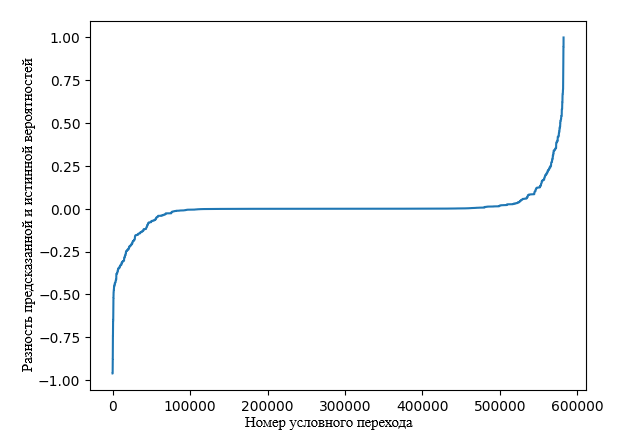
\includegraphics[scale=0.9]{PNG/prediction}
	}
	\caption{S-кривая вероятностей предсказанных переходов на тестовом пакете ExeBench}\label{fig:prediction1}
\end{figure}


\begin{table} [htbp]
	\centering
	\begin{threeparttable}% выравнивание подписи по границам таблицы
		\caption{Ускорение приложений "CPUBench fp"\phantom{} при компиляции с использованием предсказанного с помощью решающих деревьев  профиля}\label{op:pgo2}%
		\begin{tabular}{| m{5cm} | m{8cm}l |}
			\hline
			\hline
			\centering \textbf{Приложение}			 & \centering  \textbf{Ускорение} & \\
			\hline
			\centering phyml			 & \centering  0.80 & \\
			\hline
			\centering cube			 & \centering 0.89   & \\
			\hline
			\centering nektar			 & \centering 0.90  & \\
			\hline
			\centering lightgbm			 & \centering 0.95   & \\
			\hline
			\centering lammps & \centering 0.98   & \\
			\hline
			\centering phenglei & \centering 0.99   & \\
			\hline
			\centering povray 	& \centering  1.00  & \\
			\hline
			\centering openfoam 	& \centering  1.04  & \\
			\hline
			\centering gromacs 	& \centering  1.15  & \\
			\hline
			\centering   	& \centering    & \\
			\hline
			\centering Geomean 	& \centering  0.96  & \\
			\hline
			\hline
		\end{tabular}
	\end{threeparttable}
\end{table}

Качество натренированной модели можно оценить при помощи графика \ref{fig:prediction1}. По горизонтальной оси: номер условного перехода в тестовой выборке из пакета ExeBench после сортировки. По вертикальной оси: разница между предсказанной вероятностью с помощью модели и собранной при помощи инструментарии GCC. тем не менее, полученные результаты не оправдали своих ожиданий  (таблица \ref{op:pgo2}). Несмотря на улучшение производительности на тесте \textbf{gromacs} в 15 \%, большинство тестов показало деградацию  производительности. Методу требуется дальнейшее улучшение. Если вернуться к оригинальному исследованию  \cite{rotem2021profile}, то в нем обучение и замер производительности проходил на одних и тех же данных, что в нашей ситуации неприемлемо.  

Для решения проблемы деградации производительности было решено увеличить количество признаков и добавить тем самым больше информации об окружающем коде. Признаки, собираемые для перехода и условного перехода остались прежними (таблицы \ref{op:pgo_geatures1} и \ref{op:pgo_geatures2}). Однако теперь информация о базовом блоке собиралась не только для основного базового блока, а также для его наследников степени 2 (условно для детей и внуков). Количество признаков увеличилось и стало больше сотни, а размер модели вырос до нескольких мегабайт. Это помогло побороть большинство деградаций производительности (сохранилась деградация 5\% на phyml), однако уменьшило проивзодительность на тесте gromacs до 10 \%. Тем не менее, это показывает, что подход имеет место быть, а дальнейшее его улучшение возможно с улучшением модели и добавлением признаков.

\section{Разбиение условных выражений}  \label{ifsplit}
В начале главы, в разделе \ref{opt:ifconv}, упоминались существенные преимущества преобразования условных переходов. Однако в этом разделе будет продемонстрирована в некотором смысле обратная оптимизация. Рассмотрим немного упрощенный пример из теста phyml на листинге \ref{opt:ifsplit1}.
\begin{ListingEnv}[!h]
	\captiondelim{ } % разделитель идентификатора с номером от наименования
	\caption{Пример кандидата для оптимизации разбиения условных выражений из теста phyml}\label{opt:ifsplit1}
	\begin{Verb}
		if(tree->mod->ns == 4 || tree->mod->ns == 20) {	
			foo(tree);
		}
	\end{Verb}
\end{ListingEnv}

Дело в том, что такое выражение накладывает на переменную $ns$ ограничение ($ns==4$ или $ns==20$). К сожалению работа с такого рода решеткой очень затруднительна для оптимизации распространения констант. Поэтому предлагается облегчить работу таким проходам (локальному и глобальному  распространению константных выражений) трансформировав такой в листинг \ref{opt:ifsplit2}.
\begin{ListingEnv}[!h]
	\captiondelim{ } % разделитель идентификатора с номером от наименования
	\caption{Преобразованный листинг \ref{opt:ifsplit1}}\label{opt:ifsplit2}
	\begin{Verb}
		if(tree->mod->ns == 4) {	
			foo(tree);
		} else if (tree->mod->ns == 20) {
			foo(tree);
		}
	\end{Verb}
\end{ListingEnv}

Реализованная оптимизация состоит прохода по всем базовым блокам с условными выражениями.
Проход ищет выражение, содержащее логическое ИЛИ, которое содержит сравнение некоторой переменной с константой. При этом по этому условию должен происходить переход на базовый блок или цепочку базовых блоков, содержащих вызов функции,  один из аргументов которой является предикатом, либо его агрегатом. Естественно, глубина поиска агрегирования регулируется опцией (в работе была ограничена 2).Количество сравнений не  является ограничением, так как каждый раз происходит отщепление одного из вариантов. 

Такой подход может приводить к существенному увеличению размера целевого кода, поэтому оптимизация накладывает ограничения на количество инструкций внутри функции(й).

\section{Выводы по главе и замеры производительности}  \label{results}
В третьей главе  было описано более десяти различных компиляторных оптимизаций и их улучшений, которые были получены после анализа литературы в главе \ref{ch:chReview} и при помощи методологии, описанной в главе \ref{ch:chMethod}. На момент написания диссертации сообществом были приняты оптимизации, описанные в главах \ref{sec:ch2/sect1}, \ref{sec:ch2/sect2}, \ref{opt:devirt}, \ref{ch2:split_ldp_stp}, \ref{ch2:lcv}, \ref{opt:prefetch}. Автор надеется, что остальные оптимизации будут приняты в ближайшем будущем.

Результаты замеров, проведенных в полном соответствии с методологией, описанной в главе \ref{p1:method}, показаны на рисунках \ref{fig:spubench_int_speedup} и \ref{fig:spec_int_speedup}. Можно видеть, что высокие цифры увеличения производительности на тестах пакета CPUBench достигаются за счет значительного ускорения криптографического приложения openSSL. Результаты, полученные на тестах "SpecCPU int"\phantom{ } показывают ускорение за счет теста x264, который также находится в пакете CPUBench. На тестахс плавающей точкой очень хорошо видно, как предлагаемые оптимизацию перестают работать на большем числе копий. Такое поведение говорит об интенсивном использовании ресурсов памяти этими тестами. Особенно хорошо данных эффект просматривается на тесте nektar (рисунок \ref{fig:pubench_fp_speedup}). Тем не менее производительность одной копии существенно возросла, отдельные тесты достигают ускорения в 40 \%. На наборе "SpecCPU fp"\phantom{} заметного улучшения производительности не наблюдается. Единственные тест, показавший улучшение это nab.

\begin{figure}[ht]
	\centerfloat{
		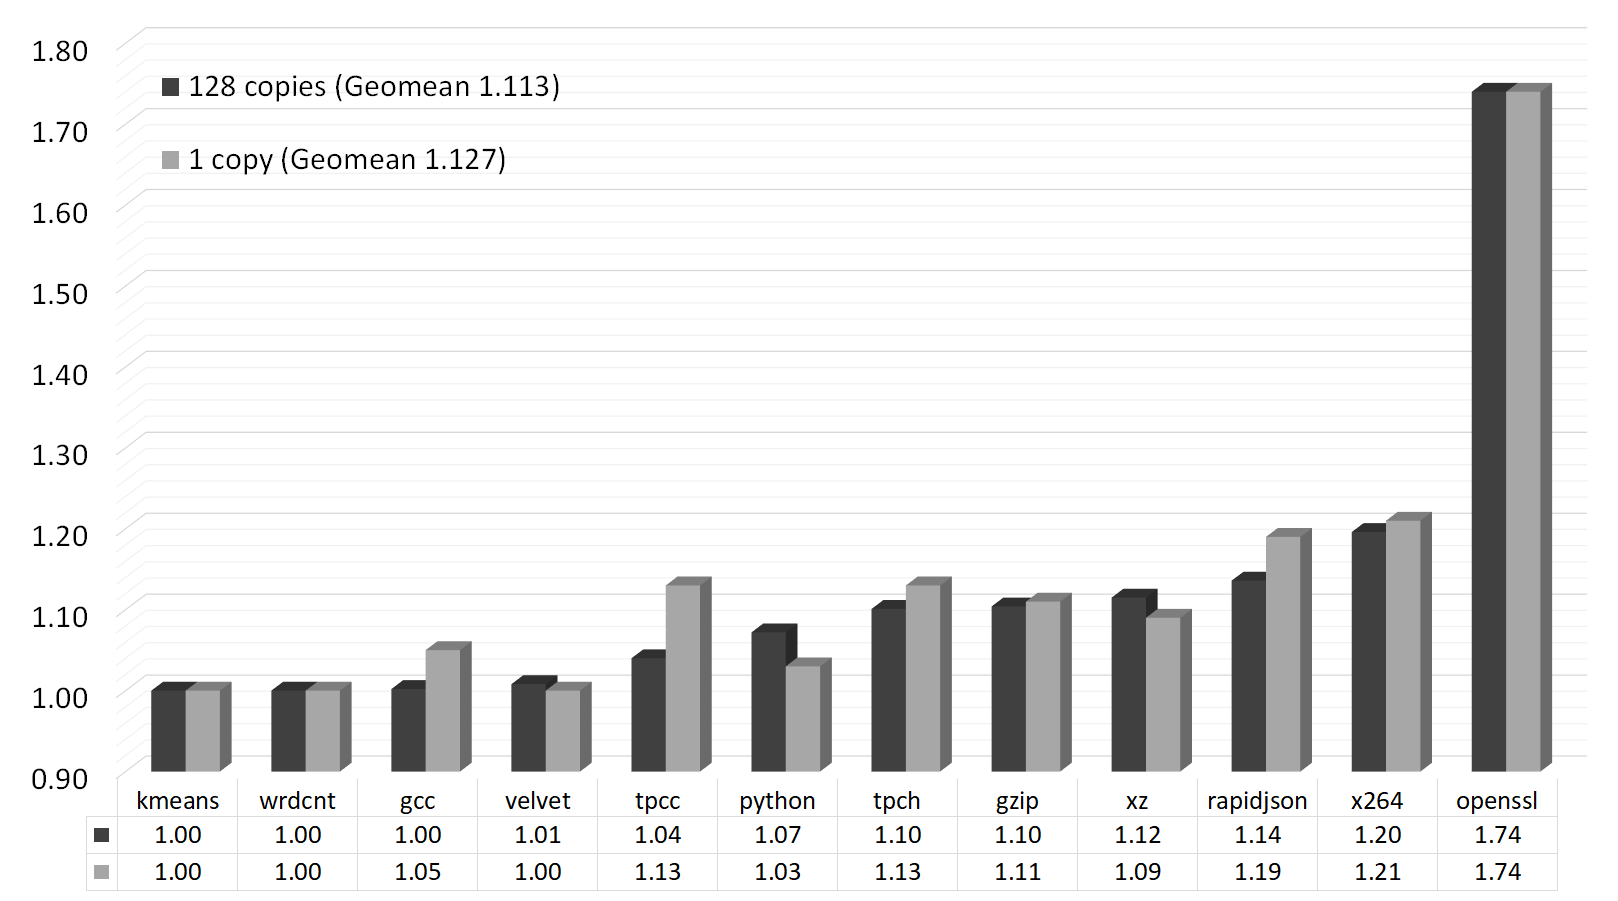
\includegraphics[scale=0.4]{PNG/speedup_combined3.png}
	}
	\caption{Результаты замеров производительности на тестах  пакета "CPUBench int"\phantom{}}\label{fig:spubench_int_speedup}
\end{figure}

\begin{figure}[ht]
	\centerfloat{
		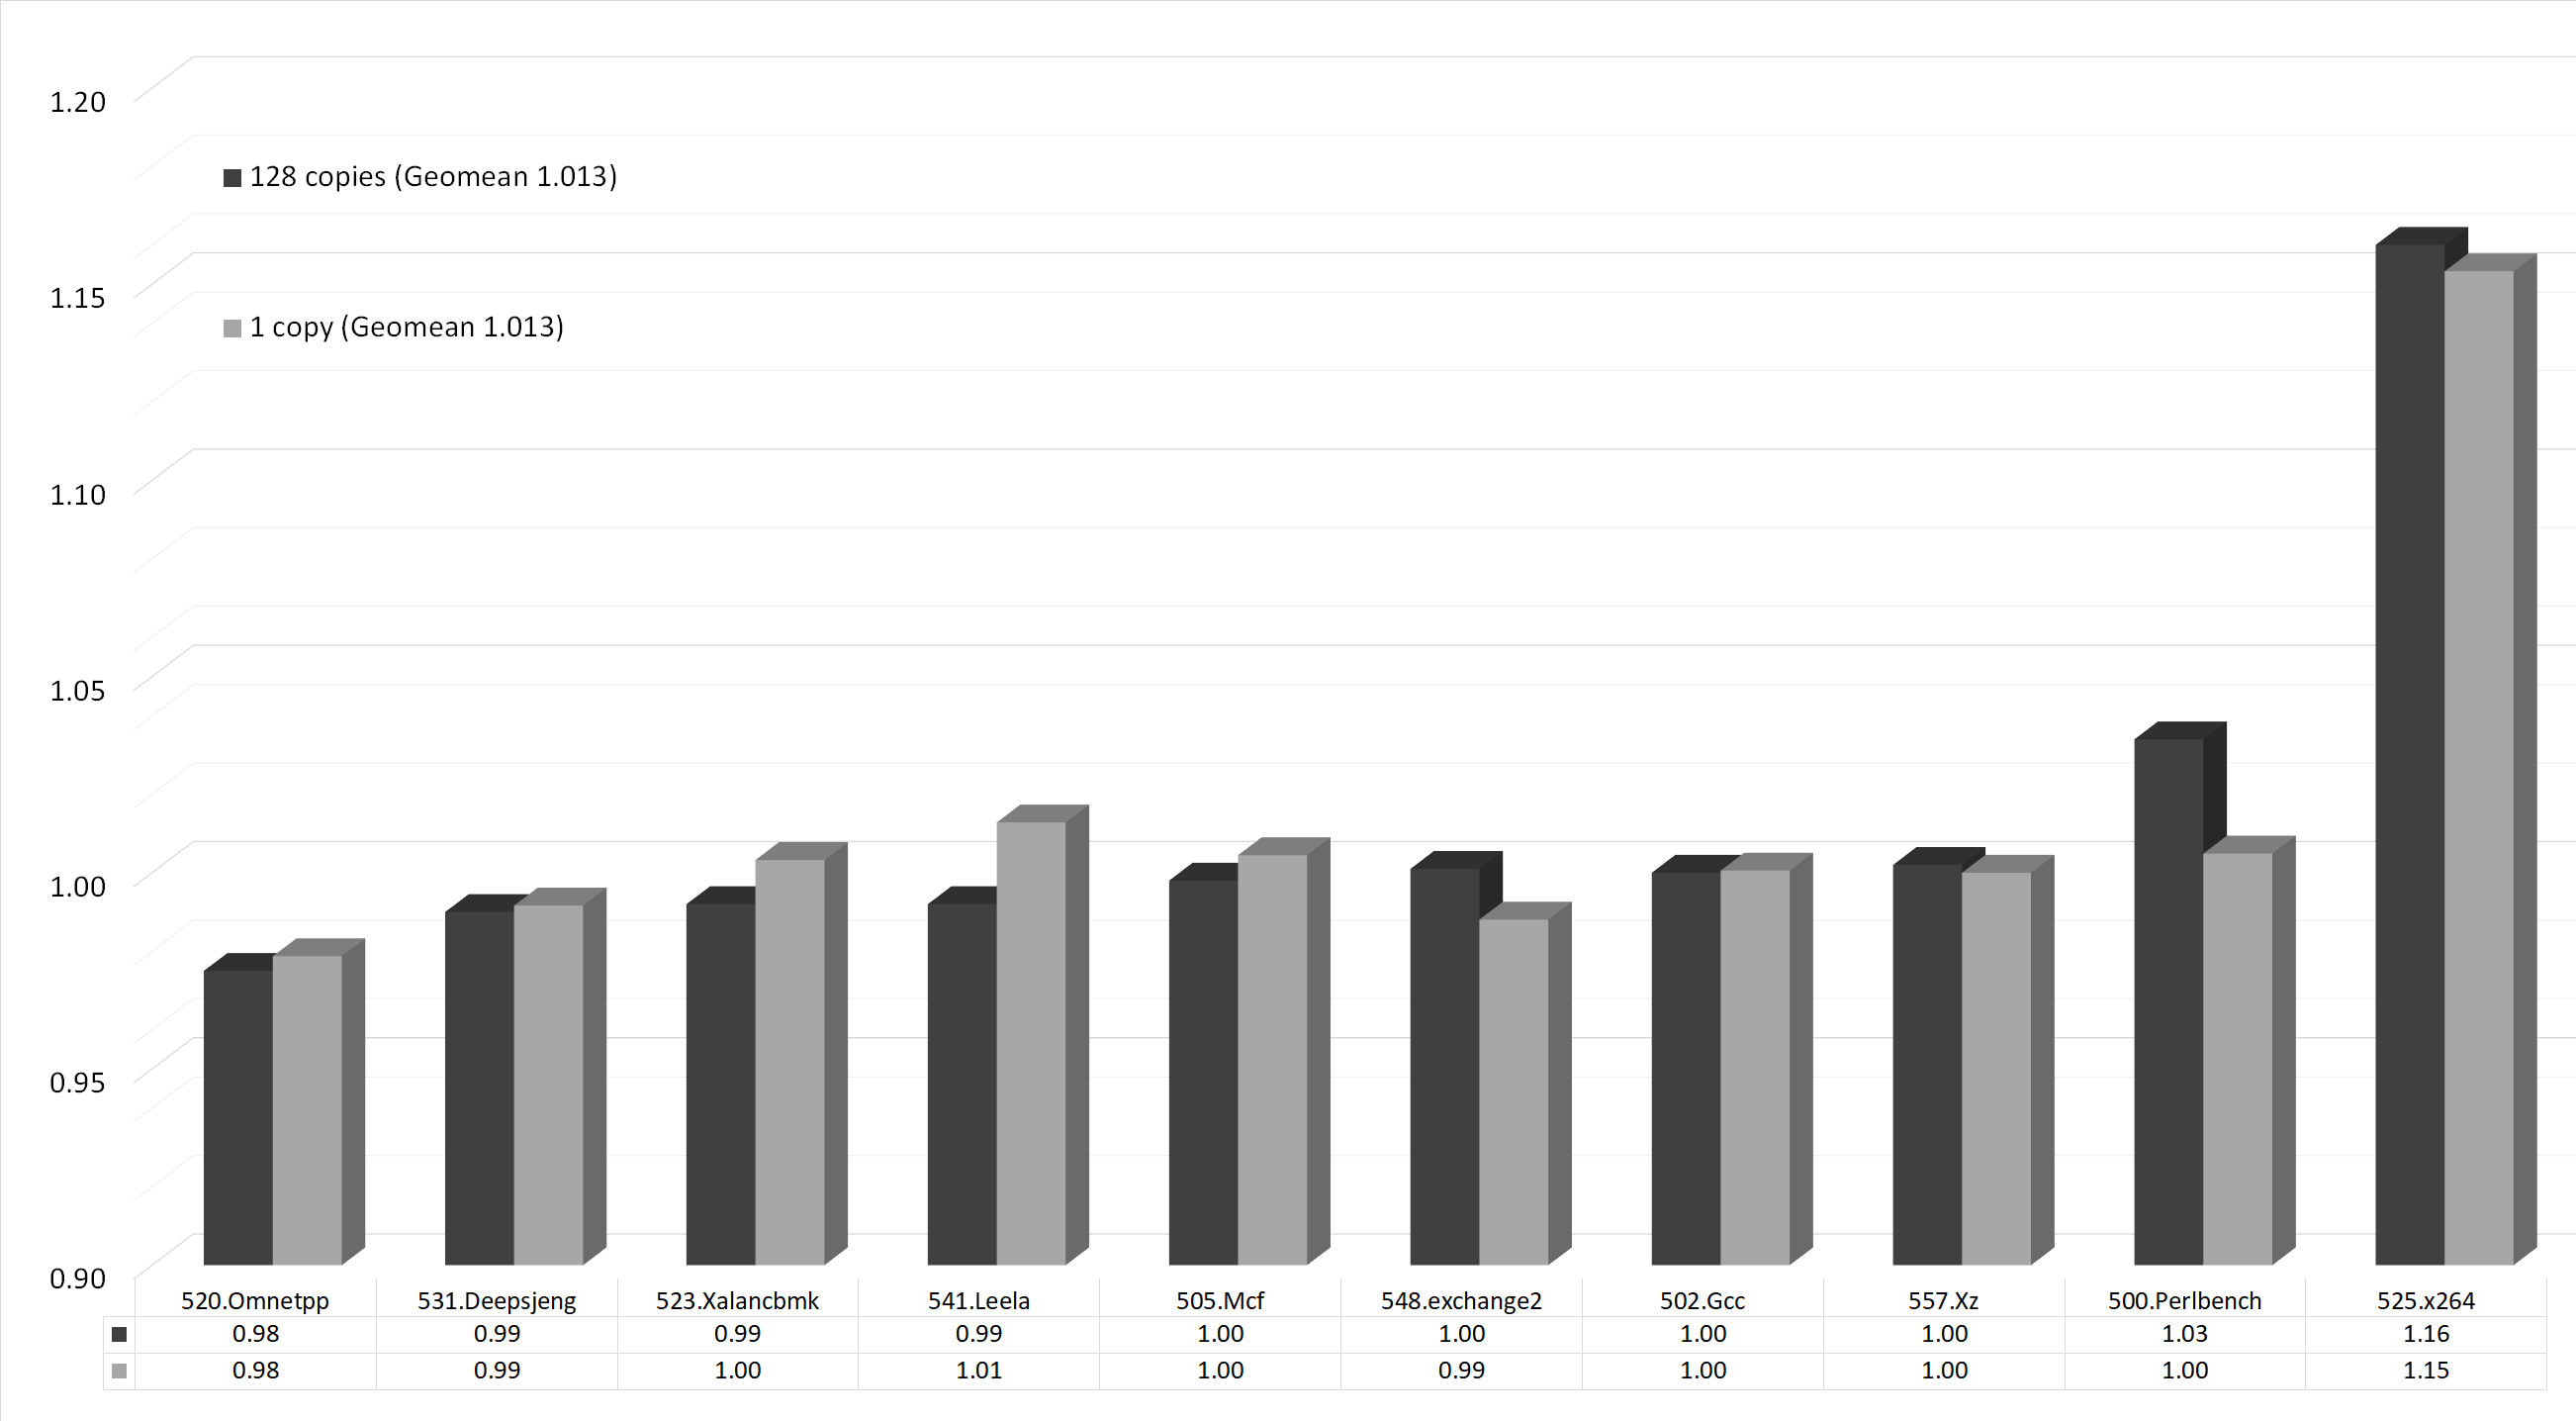
\includegraphics[scale=0.25]{PNG/spec_speedup.png}
	}
	\caption{Результаты замеров производительности на тестах пакета "SpecCPU int"\phantom{}}\label{fig:spec_int_speedup}
\end{figure}

\begin{figure}[ht]
	\centerfloat{
		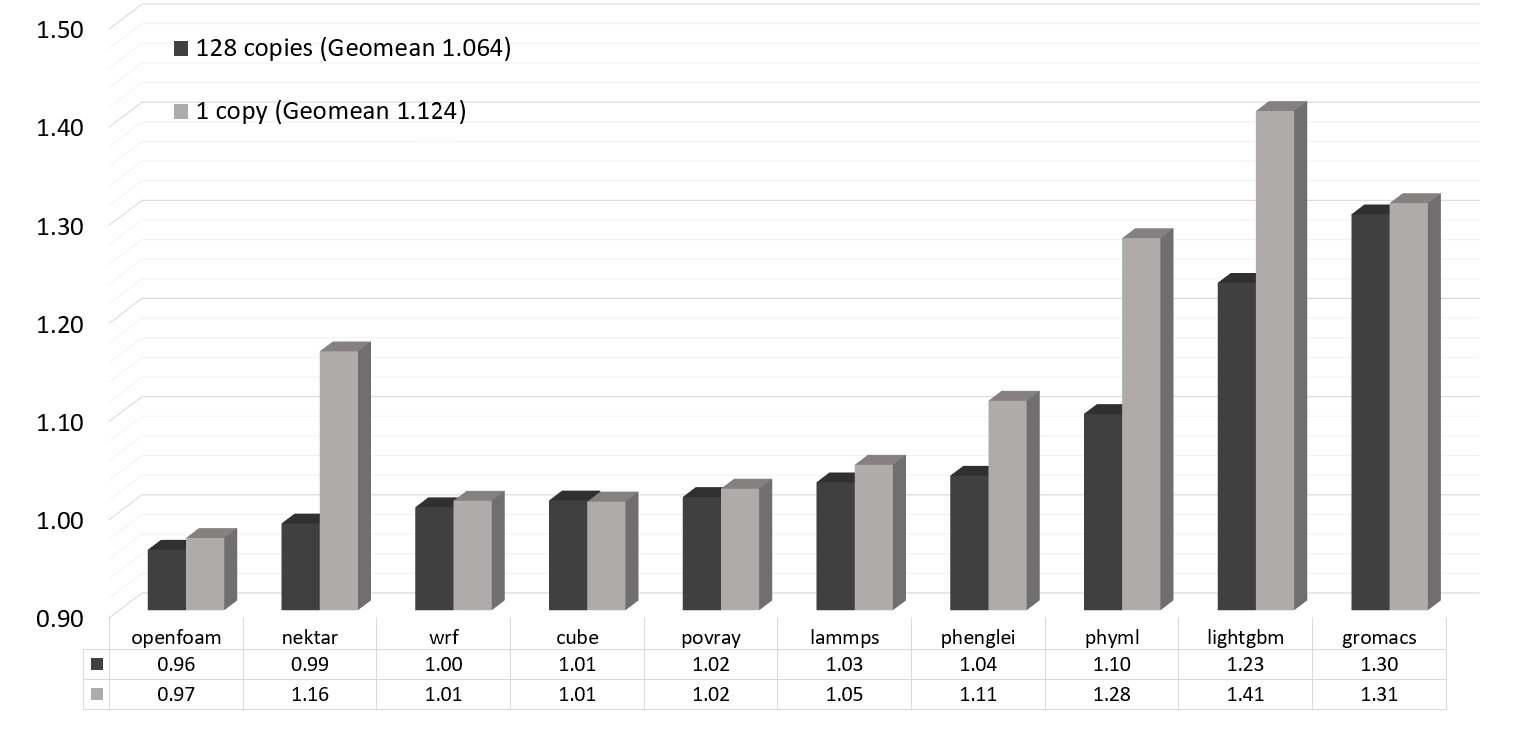
\includegraphics[scale=0.5]{PNG/speedup_combined3_fp.png}
	}
	\caption{Результаты замеров производительности на тестах  пакета "CPUBench fp"\phantom{}}\label{fig:pubench_fp_speedup}
\end{figure}

\begin{figure}[ht]
	\centerfloat{
		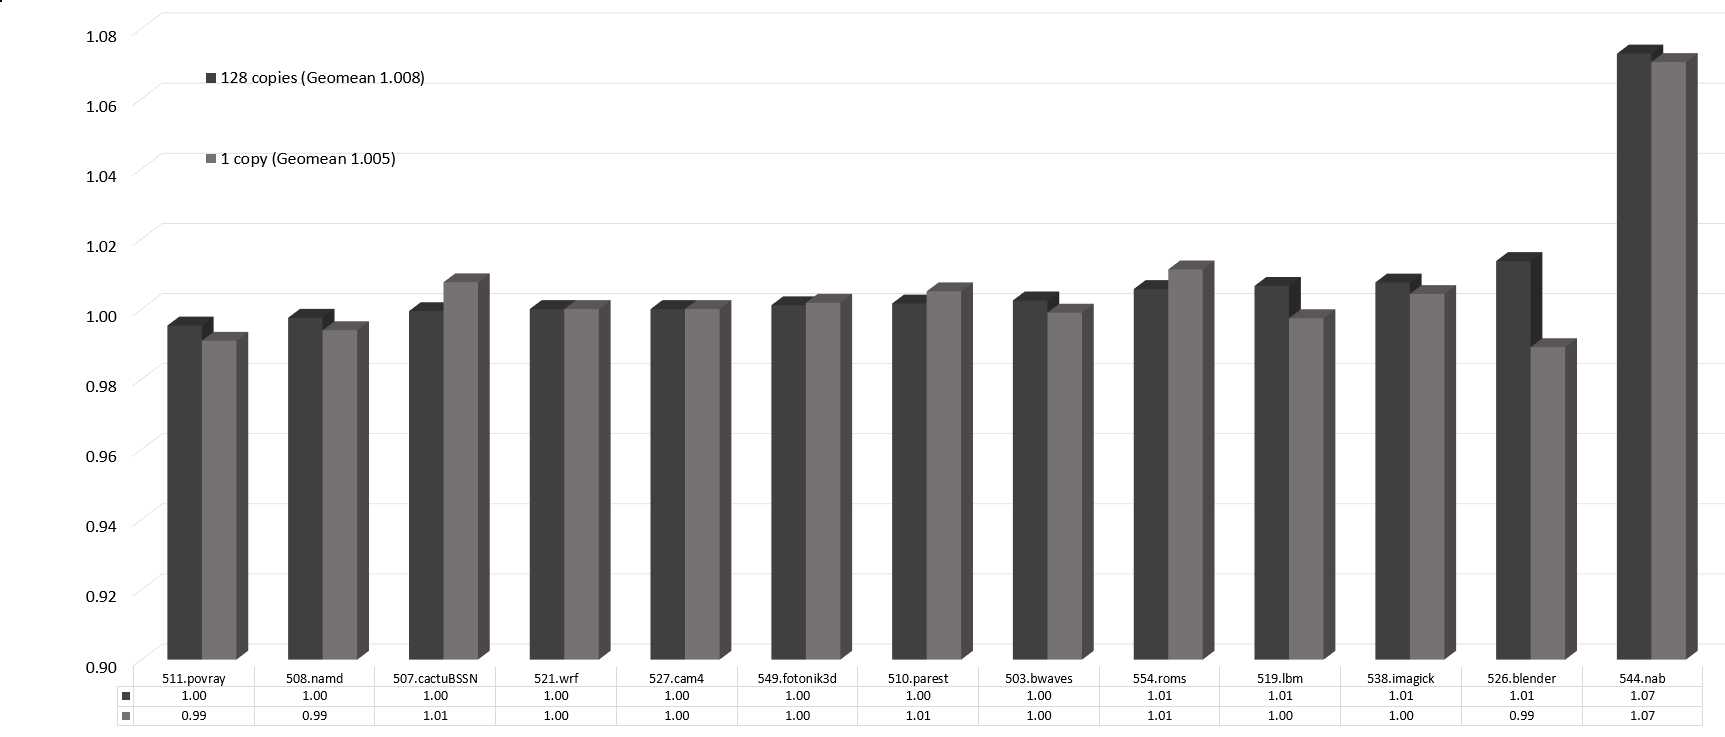
\includegraphics[scale=0.42]{PNG/spec_speedup_fp.png}
	}
	\caption{Результаты замеров производительности на тестах пакета "SpecCPU fp"\phantom{}}\label{fig:spec_fp_speedup}
\end{figure}



%\chapter{Оформление различных элементов}\label{ch:ch7}

\section{Форматирование текста}\label{sec:ch1/sec1}

Мы можем сделать \textbf{жирный текст} и \textit{курсив}.

\section{Ссылки}\label{sec:ch1/sec2}

Сошлёмся на библиографию.
Одна ссылка: \cite[с.~54]{Sokolov}\cite[с.~36]{Gaidaenko}.
Две ссылки: \cite{Sokolov,Gaidaenko}.
Ссылка на собственные работы: \cite{vakbib1, confbib2}.
Много ссылок: %\cite[с.~54]{Lermontov,Management,Borozda} % такой «фокус»
%вызывает biblatex warning относительно опции sortcites, потому что неясно, к
%какому источнику относится уточнение о страницах, а bibtex об этой проблеме
%даже не предупреждает
\cite{Lermontov, Management, Borozda, Marketing, Constitution, FamilyCode,
    Gost.7.0.53, Razumovski, Lagkueva, Pokrovski, Methodology, Berestova,
    Kriger}%
\ifnumequal{\value{bibliosel}}{0}{% Примеры для bibtex8
    \cite{Sirotko, Lukina, Encyclopedia, Nasirova}%
}{% Примеры для biblatex через движок biber
    \cite{Sirotko2, Lukina2, Encyclopedia2, Nasirova2}%
}%
.
И~ещё немного ссылок:~\cite{Article,Book,Booklet,Conference,Inbook,Incollection,Manual,Mastersthesis,
    Misc,Phdthesis,Proceedings,Techreport,Unpublished}
% Следует обратить внимание, что пробел после запятой внутри \cite{}
% обрабатывается ожидаемо, а пробел перед запятой, может вызывать проблемы при
% обработке ссылок.
\cite{medvedev2006jelektronnye, CEAT:CEAT581, doi:10.1080/01932691.2010.513279,
    Gosele1999161,Li2007StressAnalysis, Shoji199895, test:eisner-sample,
    test:eisner-sample-shorted, AB_patent_Pomerantz_1968, iofis_patent1960}%
\ifnumequal{\value{bibliosel}}{0}{% Примеры для bibtex8
}{% Примеры для biblatex через движок biber
    \cite{patent2h, patent3h, patent2}%
}%
.

\ifnumequal{\value{bibliosel}}{0}{% Примеры для bibtex8
Попытка реализовать несколько ссылок на конкретные страницы
для \texttt{bibtex} реализации библиографии:
[\citenum{Sokolov}, с.~54; \citenum{Gaidaenko}, с.~36].
}{% Примеры для biblatex через движок biber
Несколько источников (мультицитата):
% Тут специально написано по-разному тире, для демонстрации, что
% применение специальных тире в настоящий момент в biblatex приводит к непоказу
% "с.".
\cites[vii--x, 5, 7]{Sokolov}[v"--~x, 25, 526]{Gaidaenko}[vii--x, 5, 7]{Techreport},
работает только в \texttt{biblatex} реализации библиографии.
}%

Ссылки на собственные работы:~\cite{vakbib1, confbib1}.

Сошлёмся на приложения: Приложение~\cref{app:A}, Приложение~\cref{app:B2}.

Сошлёмся на формулу: формула~\cref{eq:equation1}.

Сошлёмся на изображение: рисунок~\cref{fig:knuth}.

Стандартной практикой является добавление к ссылкам префикса, характеризующего тип элемента.
Это не является строгим требованием, но~позволяет лучше ориентироваться в документах большого размера.
Например, для ссылок на~рисунки используется префикс \textit{fig},
для ссылки на~таблицу "--- \textit{tab}.

В таблице \cref{tab:tab_pref} приложения~\cref{app:B4} приведён список рекомендуемых
к использованию стандартных префиксов.

В некоторых ситуациях возникает необходимость отойти от требований ГОСТ по оформлению ссылок на
литературу.
В таком случае можно воспользоваться дополнительными опциями пакета \verb+biblatex+.

Например, в ссылке на книгу~\cite{sobenin_kdv} использование опции \verb+maxnames=4+ позволяет
вывести имена всех четырёх авторов.
По ГОСТ имена последних трёх авторов опускаются.

Кроме того, часто возникают проблемы с транслитерованными инициалами. Некоторые буквы русского
алфавита по правилам транслитерации записываются двумя буквами латинского алфавита (ю-yu, ё-yo и
т.д.).
Такие инициалы \verb+biblatex+ будет сокращать до одной буквы, что неверно.
Поправить его работу можно использовав опцию \verb+giveninits=false+.
Пример использования этой опции можно видеть в ссылке~\cite{initials}.

\section{Формулы}\label{sec:ch7/sec3}

Благодаря пакету \textit{icomma}, \LaTeX~одинаково хорошо воспринимает
в~качестве десятичного разделителя и запятую (\(3,1415\)), и точку (\(3.1415\)).

\subsection{Ненумерованные одиночные формулы}\label{subsec:ch7/sec3/sub1}

Вот так может выглядеть формула, которую необходимо вставить в~строку
по~тексту: \(x \approx \sin x\) при \(x \to 0\).

А вот так выглядит ненумерованная отдельностоящая формула c подстрочными
и надстрочными индексами:
\[
    (x_1+x_2)^2 = x_1^2 + 2 x_1 x_2 + x_2^2
\]

Формула с неопределенным интегралом:
\[
    \int f(\alpha+x)=\sum\beta
\]

При использовании дробей формулы могут получаться очень высокие:
\[
    \frac{1}{\sqrt{2}+
        \displaystyle\frac{1}{\sqrt{2}+
            \displaystyle\frac{1}{\sqrt{2}+\cdots}}}
\]

В формулах можно использовать греческие буквы:
%Все \original... команды заранее, ради этого примера, определены в Dissertation\userstyles.tex
\[
    \alpha\beta\gamma\delta\originalepsilon\epsilon\zeta\eta\theta%
    \vartheta\iota\kappa\varkappa\lambda\mu\nu\xi\pi\varpi\rho\varrho%
    \sigma\varsigma\tau\upsilon\originalphi\phi\chi\psi\omega\Gamma\Delta%
    \Theta\Lambda\Xi\Pi\Sigma\Upsilon\Phi\Psi\Omega
\]
\[%https://texfaq.org/FAQ-boldgreek
    \boldsymbol{\alpha\beta\gamma\delta\originalepsilon\epsilon\zeta\eta%
        \theta\vartheta\iota\kappa\varkappa\lambda\mu\nu\xi\pi\varpi\rho%
        \varrho\sigma\varsigma\tau\upsilon\originalphi\phi\chi\psi\omega\Gamma%
        \Delta\Theta\Lambda\Xi\Pi\Sigma\Upsilon\Phi\Psi\Omega}
\]

Для добавления формул можно использовать пары \verb+$+\dots\verb+$+ и \verb+$$+\dots\verb+$$+,
но~они считаются устаревшими.
Лучше использовать их функциональные аналоги \verb+\(+\dots\verb+\)+ и \verb+\[+\dots\verb+\]+.

\subsection{Ненумерованные многострочные формулы}\label{subsec:ch7/sec3/sub2}

Вот так можно написать две формулы, не нумеруя их, чтобы знаки <<равно>> были
строго друг под другом:
\begin{align}
    f_W & =  \min \left( 1, \max \left( 0, \frac{W_{soil} / W_{max}}{W_{crit}} \right)  \right), \nonumber \\
    f_T & =  \min \left( 1, \max \left( 0, \frac{T_s / T_{melt}}{T_{crit}} \right)  \right), \nonumber
\end{align}

Выровнять систему ещё и по переменной \( x \) можно, используя окружение
\verb|alignedat| из пакета \verb|amsmath|. Вот так:
\[
|x| = \left\{
\begin{alignedat}{2}
    &&x, \quad &\text{eсли } x\geqslant 0 \\
    &-&x, \quad & \text{eсли } x<0
\end{alignedat}
\right.
\]
Здесь первый амперсанд (в исходном \LaTeX\ описании формулы) означает
выравнивание по~левому краю, второй "--- по~\( x \), а~третий "--- по~слову
<<если>>. Команда \verb|\quad| делает большой горизонтальный пробел.

Ещё вариант:
\[
    |x|=
    \begin{cases}
        \phantom{-}x, \text{если } x \geqslant 0 \\
        -x, \text{если } x<0
    \end{cases}
\]

Кроме того, для  нумерованных формул \verb|alignedat| делает вертикальное
выравнивание номера формулы по центру формулы. Например, выравнивание
компонент вектора:
\begin{equation}
    \label{eq:2p3}
    \begin{alignedat}{2}
        {\mathbf{N}}_{o1n}^{(j)} = \,{\sin} \phi\,n\!\left(n+1\right)
        {\sin}\theta\,
        \pi_n\!\left({\cos} \theta\right)
        \frac{
        z_n^{(j)}\!\left( \rho \right)
        }{\rho}\,
        &{\boldsymbol{\hat{\mathrm e}}}_{r}\,+   \\
        +\,
        {\sin} \phi\,
        \tau_n\!\left({\cos} \theta\right)
        \frac{
        \left[\rho z_n^{(j)}\!\left( \rho \right)\right]^{\prime}
        }{\rho}\,
        &{\boldsymbol{\hat{\mathrm e}}}_{\theta}\,+   \\
        +\,
        {\cos} \phi\,
        \pi_n\!\left({\cos} \theta\right)
        \frac{
        \left[\rho z_n^{(j)}\!\left( \rho \right)\right]^{\prime}
        }{\rho}\,
        &{\boldsymbol{\hat{\mathrm e}}}_{\phi}\:.
    \end{alignedat}
\end{equation}

Ещё об отступах. Иногда для лучшей <<читаемости>> формул полезно
немного исправить стандартные интервалы \LaTeX\ с учётом логической
структуры самой формулы. Например в формуле~\cref{eq:2p3} добавлен
небольшой отступ \verb+\,+ между основными сомножителями, ниже
результат применения всех вариантов отступа:
\begin{align*}
    \backslash!             & \quad f(x) = x^2\! +3x\! +2         \\
    \mbox{по-умолчанию}     & \quad f(x) = x^2+3x+2               \\
    \backslash,             & \quad f(x) = x^2\, +3x\, +2         \\
    \backslash{:}           & \quad f(x) = x^2\: +3x\: +2         \\
    \backslash;             & \quad f(x) = x^2\; +3x\; +2         \\
    \backslash \mbox{space} & \quad f(x) = x^2\ +3x\ +2           \\
    \backslash \mbox{quad}  & \quad f(x) = x^2\quad +3x\quad +2   \\
    \backslash \mbox{qquad} & \quad f(x) = x^2\qquad +3x\qquad +2
\end{align*}

Можно использовать разные математические алфавиты:
\begin{align}
    \mathcal{ABCDEFGHIJKLMNOPQRSTUVWXYZ} \nonumber  \\
    \mathfrak{ABCDEFGHIJKLMNOPQRSTUVWXYZ} \nonumber \\
    \mathbb{ABCDEFGHIJKLMNOPQRSTUVWXYZ} \nonumber
\end{align}

Посмотрим на систему уравнений на примере аттрактора Лоренца:

\[
\left\{
\begin{array}{rl}
    \dot x = & \sigma (y-x)  \\
    \dot y = & x (r - z) - y \\
    \dot z = & xy - bz
\end{array}
\right.
\]

А для вёрстки матриц удобно использовать многоточия:
\[
    \left(
        \begin{array}{ccc}
            a_{11} & \ldots & a_{1n} \\
            \vdots & \ddots & \vdots \\
            a_{n1} & \ldots & a_{nn} \\
        \end{array}
    \right)
\]

\subsection{Нумерованные формулы}\label{subsec:ch7/sec3/sub3}

А вот так пишется нумерованная формула:
\begin{equation}
    \label{eq:equation1}
    e = \lim_{n \to \infty} \left( 1+\frac{1}{n} \right) ^n
\end{equation}

Нумерованных формул может быть несколько:
\begin{equation}
    \label{eq:equation2}
    \lim_{n \to \infty} \sum_{k=1}^n \frac{1}{k^2} = \frac{\pi^2}{6}
\end{equation}

Впоследствии на формулы~\cref{eq:equation1, eq:equation2} можно ссылаться.

Сделать так, чтобы номер формулы стоял напротив средней строки, можно,
используя окружение \verb|multlined| (пакет \verb|mathtools|) вместо
\verb|multline| внутри окружения \verb|equation|. Вот так:
\begin{equation} % \tag{S} % tag - вписывает свой текст
    \label{eq:equation3}
    \begin{multlined}
        1+ 2+3+4+5+6+7+\dots + \\
        + 50+51+52+53+54+55+56+57 + \dots + \\
        + 96+97+98+99+100=5050
    \end{multlined}
\end{equation}

Уравнения~\cref{eq:subeq_1,eq:subeq_2} демонстрируют возможности
окружения \verb|\subequations|.
\begin{subequations}
    \label{eq:subeq_1}
    \begin{gather}
        y = x^2 + 1 \label{eq:subeq_1-1} \\
        y = 2 x^2 - x + 1 \label{eq:subeq_1-2}
    \end{gather}
\end{subequations}
Ссылки на отдельные уравнения~\cref{eq:subeq_1-1,eq:subeq_1-2,eq:subeq_2-1}.
\begin{subequations}
    \label{eq:subeq_2}
    \begin{align}
        y & = x^3 + x^2 + x + 1 \label{eq:subeq_2-1} \\
        y & = x^2
    \end{align}
\end{subequations}

\subsection{Форматирование чисел и размерностей величин}\label{sec:units}

Числа форматируются при помощи команды \verb|\num|:
\num{5,3};
\num{2,3e8};
\num{12345,67890};
\num{2,6 d4};
\num{1+-2i};
\num{.3e45};
\num[exponent-base=2]{5 e64};
\num[exponent-base=2,exponent-to-prefix]{5 e64};
\num{1.654 x 2.34 x 3.430}
\num{1 2 x 3 / 4}.
Для написания последовательности чисел можно использовать команды \verb|\numlist| и \verb|\numrange|:
\numlist{10;30;50;70}; \numrange{10}{30}.
Значения углов можно форматировать при помощи команды \verb|\ang|:
\ang{2.67};
\ang{30,3};
\ang{-1;;};
\ang{;-2;};
\ang{;;-3};
\ang{300;10;1}.

Обратите внимание, что ГОСТ запрещает использование знака <<->> для обозначения отрицательных чисел
за исключением формул, таблиц и~рисунков.
Вместо него следует использовать слово <<минус>>.

Размерности можно записывать при помощи команд \verb|\si| и \verb|\SI|:
\si{\farad\squared\lumen\candela};
\si{\joule\per\mole\per\kelvin};
\si[per-mode = symbol-or-fraction]{\joule\per\mole\per\kelvin};
\si{\metre\per\second\squared};
\SI{0.10(5)}{\neper};
\SI{1.2-3i e5}{\joule\per\mole\per\kelvin};
\SIlist{1;2;3;4}{\tesla};
\SIrange{50}{100}{\volt}.
Список единиц измерений приведён в таблицах~\cref{tab:unit:base,
    tab:unit:derived,tab:unit:accepted,tab:unit:physical,tab:unit:other}.
Приставки единиц приведены в~таблице~\cref{tab:unit:prefix}.

С дополнительными опциями форматирования можно ознакомиться в~описании пакета \texttt{siunitx};
изменить или добавить единицы измерений можно в~файле \texttt{siunitx.cfg}.

\begin{table}
    \centering
    \captionsetup{justification=centering} % выравнивание подписи по-центру
    \caption{Основные величины СИ}\label{tab:unit:base}
    \begin{tabular}{llc}
        \toprule
        Название  & Команда                 & Символ         \\
        \midrule
        Ампер     & \verb|\ampere| & \si{\ampere}   \\
        Кандела   & \verb|\candela| & \si{\candela}  \\
        Кельвин   & \verb|\kelvin| & \si{\kelvin}   \\
        Килограмм & \verb|\kilogram| & \si{\kilogram} \\
        Метр      & \verb|\metre| & \si{\metre}    \\
        Моль      & \verb|\mole| & \si{\mole}     \\
        Секунда   & \verb|\second| & \si{\second}   \\
        \bottomrule
    \end{tabular}
\end{table}

\begin{table}
    \small
    \centering
    \begin{threeparttable}% выравнивание подписи по границам таблицы
        \caption{Производные единицы СИ}\label{tab:unit:derived}
        \begin{tabular}{llc|llc}
            \toprule
            Название       & Команда                 & Символ              & Название & Команда & Символ \\
            \midrule
            Беккерель      & \verb|\becquerel| & \si{\becquerel}     &
            Ньютон         & \verb|\newton| & \si{\newton}                                      \\
            Градус Цельсия & \verb|\degreeCelsius| & \si{\degreeCelsius} &
            Ом             & \verb|\ohm| & \si{\ohm}                                         \\
            Кулон          & \verb|\coulomb| & \si{\coulomb}       &
            Паскаль        & \verb|\pascal| & \si{\pascal}                                      \\
            Фарад          & \verb|\farad| & \si{\farad}         &
            Радиан         & \verb|\radian| & \si{\radian}                                      \\
            Грей           & \verb|\gray| & \si{\gray}          &
            Сименс         & \verb|\siemens| & \si{\siemens}                                     \\
            Герц           & \verb|\hertz| & \si{\hertz}         &
            Зиверт         & \verb|\sievert| & \si{\sievert}                                     \\
            Генри          & \verb|\henry| & \si{\henry}         &
            Стерадиан      & \verb|\steradian| & \si{\steradian}                                   \\
            Джоуль         & \verb|\joule| & \si{\joule}         &
            Тесла          & \verb|\tesla| & \si{\tesla}                                       \\
            Катал          & \verb|\katal| & \si{\katal}         &
            Вольт          & \verb|\volt| & \si{\volt}                                        \\
            Люмен          & \verb|\lumen| & \si{\lumen}         &
            Ватт           & \verb|\watt| & \si{\watt}                                        \\
            Люкс           & \verb|\lux| & \si{\lux}           &
            Вебер          & \verb|\weber| & \si{\weber}                                       \\
            \bottomrule
        \end{tabular}
    \end{threeparttable}
\end{table}

\begin{table}
    \centering
    \begin{threeparttable}% выравнивание подписи по границам таблицы
        \caption{Внесистемные единицы}\label{tab:unit:accepted}

        \begin{tabular}{llc}
            \toprule
            Название        & Команда                 & Символ          \\
            \midrule
            День            & \verb|\day| & \si{\day}       \\
            Градус          & \verb|\degree| & \si{\degree}    \\
            Гектар          & \verb|\hectare| & \si{\hectare}   \\
            Час             & \verb|\hour| & \si{\hour}      \\
            Литр            & \verb|\litre| & \si{\litre}     \\
            Угловая минута  & \verb|\arcminute| & \si{\arcminute} \\
            Угловая секунда & \verb|\arcsecond| & \si{\arcsecond} \\ %
            Минута          & \verb|\minute| & \si{\minute}    \\
            Тонна           & \verb|\tonne| & \si{\tonne}     \\
            \bottomrule
        \end{tabular}
    \end{threeparttable}
\end{table}

\begin{table}
    \centering
    \captionsetup{justification=centering}
    \caption{Внесистемные единицы, получаемые из эксперимента}\label{tab:unit:physical}
    \begin{tabular}{llc}
        \toprule
        Название                & Команда                 & Символ                 \\
        \midrule
        Астрономическая единица & \verb|\astronomicalunit| & \si{\astronomicalunit} \\
        Атомная единица массы   & \verb|\atomicmassunit| & \si{\atomicmassunit}   \\
        Боровский радиус        & \verb|\bohr| & \si{\bohr}             \\
        Скорость света          & \verb|\clight| & \si{\clight}           \\
        Дальтон                 & \verb|\dalton| & \si{\dalton}           \\
        Масса электрона         & \verb|\electronmass| & \si{\electronmass}     \\
        Электрон Вольт          & \verb|\electronvolt| & \si{\electronvolt}     \\
        Элементарный заряд      & \verb|\elementarycharge| & \si{\elementarycharge} \\
        Энергия Хартри          & \verb|\hartree| & \si{\hartree}          \\
        Постоянная Планка       & \verb|\planckbar| & \si{\planckbar}        \\
        \bottomrule
    \end{tabular}
\end{table}

\begin{table}
    \centering
    \begin{threeparttable}% выравнивание подписи по границам таблицы
        \caption{Другие внесистемные единицы}\label{tab:unit:other}
        \begin{tabular}{llc}
            \toprule
            Название                  & Команда                 & Символ             \\
            \midrule
            Ангстрем                  & \verb|\angstrom| & \si{\angstrom}     \\
            Бар                       & \verb|\bar| & \si{\bar}          \\
            Барн                      & \verb|\barn| & \si{\barn}         \\
            Бел                       & \verb|\bel| & \si{\bel}          \\
            Децибел                   & \verb|\decibel| & \si{\decibel}      \\
            Узел                      & \verb|\knot| & \si{\knot}         \\
            Миллиметр ртутного столба & \verb|\mmHg| & \si{\mmHg}         \\
            Морская миля              & \verb|\nauticalmile| & \si{\nauticalmile} \\
            Непер                     & \verb|\neper| & \si{\neper}        \\
            \bottomrule
        \end{tabular}
    \end{threeparttable}
\end{table}

\begin{table}
    \small
    \centering
    \begin{threeparttable}% выравнивание подписи по границам таблицы
        \caption{Приставки СИ}\label{tab:unit:prefix}
        \begin{tabular}{llcc|llcc}
            \toprule
            Приставка & Команда                  & Символ      & Степень &
            Приставка & Команда                  & Символ      & Степень   \\
            \midrule
            Иокто     & \verb|\yocto|  & \si{\yocto} & -24     &
            Дека      & \verb|\deca|  & \si{\deca}  & 1         \\
            Зепто     & \verb|\zepto|  & \si{\zepto} & -21     &
            Гекто     & \verb|\hecto|  & \si{\hecto} & 2         \\
            Атто      & \verb|\atto|  & \si{\atto}  & -18     &
            Кило      & \verb|\kilo|  & \si{\kilo}  & 3         \\
            Фемто     & \verb|\femto|  & \si{\femto} & -15     &
            Мега      & \verb|\mega|  & \si{\mega}  & 6         \\
            Пико      & \verb|\pico|  & \si{\pico}  & -12     &
            Гига      & \verb|\giga|  & \si{\giga}  & 9         \\
            Нано      & \verb|\nano|  & \si{\nano}  & -9      &
            Терра     & \verb|\tera|  & \si{\tera}  & 12        \\
            Микро     & \verb|\micro|  & \si{\micro} & -6      &
            Пета      & \verb|\peta|  & \si{\peta}  & 15        \\
            Милли     & \verb|\milli|  & \si{\milli} & -3      &
            Екса      & \verb|\exa|  & \si{\exa}   & 18        \\
            Санти     & \verb|\centi|  & \si{\centi} & -2      &
            Зетта     & \verb|\zetta|  & \si{\zetta} & 21        \\
            Деци      & \verb|\deci| & \si{\deci}  & -1      &
            Иотта     & \verb|\yotta| & \si{\yotta} & 24        \\
            \bottomrule
        \end{tabular}
    \end{threeparttable}
\end{table}

\subsection{Заголовки с формулами: \texorpdfstring{\(a^2 + b^2 = c^2\)}{%
        a\texttwosuperior\ + b\texttwosuperior\ = c\texttwosuperior},
    \texorpdfstring{\(\left\vert\textrm{{Im}}\Sigma\left(
            \protect\varepsilon\right)\right\vert\approx const\)}{|ImΣ (ε)| ≈ const},
    \texorpdfstring{\(\sigma_{xx}^{(1)}\)}{σ\_\{xx\}\textasciicircum\{(1)\}}
}\label{subsec:with_math}

Пакет \texttt{hyperref} берёт текст для закладок в pdf-файле из~аргументов
команд типа \verb|\section|, которые могут содержать математические формулы,
а~также изменения цвета текста или шрифта, которые не отображаются в~закладках.
Чтобы использование формул в заголовках не вызывало в~логе компиляции появление
предупреждений типа <<\texttt{Token not allowed in~a~PDF string
    (Unicode):(hyperref) removing...}>>, следует использовать конструкцию
\verb|\texorpdfstring{}{}|, где в~первых фигурных скобках указывается
формула, а~во~вторых "--- запись формулы для закладок.

\section{Рецензирование текста}\label{sec:markup}

В шаблоне для диссертации и автореферата заданы команды рецензирования.
Они видны при компиляции шаблона в режиме черновика или при установке
соответствующей настройки (\verb+showmarkup+) в~файле \verb+common/setup.tex+.

Команда \verb+\todo+ отмечает текст красным цветом.
\todo{Например, так.}

Команда \verb+\note+ позволяет выбрать цвет текста.
\note{Чёрный, } \note[red]{красный, } \note[green]{зелёный, }
\note[blue]{синий.} \note[orange]{Обратите внимание на ширину и расстановку
    формирующихся пробелов, в~результате приведённой записи (зависит также
    от~применяемого компилятора).}

Окружение \verb+commentbox+ также позволяет выбрать цвет.

\begin{commentbox}[red]
    Красный текст.

    Несколько параграфов красного текста.
\end{commentbox}

\begin{commentbox}[blue]
    Синяя формула.

    \begin{equation}
        \alpha + \beta = \gamma
    \end{equation}
\end{commentbox}

\verb+commentbox+ позволяет закомментировать участок кода в~режиме чистовика.
Чтобы убрать кусок кода для всех режимов, можно использовать окружение
\verb+comment+.

\begin{comment}
Этот текст всегда скрыт.
\end{comment}

\section{Работа со списком сокращений и~условных обозначений}\label{sec:acronyms}

С помощью пакета \texttt{nomencl} можно создавать удобный сортированный список
сокращений и условных обозначений во время написания текста. Вызов
\verb+\nomenclature+ добавляет нужный символ или сокращение с~описанием
в~список, который затем печатается вызовом \verb+\printnomenclature+
в~соответствующем разделе.
Для того, чтобы эти операции прошли, потребуется дополнительный вызов
\verb+makeindex -s nomencl.ist -o %.nls %.nlo+ в~командной строке, где вместо
\verb+%+ следует подставить имя главного файла проекта (\verb+dissertation+
для этого шаблона).
Затем потребуется один или два дополнительных вызова компилятора проекта.
\begin{equation}
    \omega = c k,
\end{equation}
где \( \omega \) "--- частота света, \( c \) "--- скорость света, \( k \) "---
модуль волнового вектора.
\nomenclature{\(\omega\)}{частота света\nomrefeq}
\nomenclature{\(c\)}{скорость света\nomrefpage}
\nomenclature{\(k\)}{модуль волнового вектора\nomrefeqpage}
Использование
\begin{verbatim}
\nomenclature{\(\omega\)}{частота света\nomrefeq}
\nomenclature{\(c\)}{скорость света\nomrefpage}
\nomenclature{\(k\)}{модуль волнового вектора\nomrefeqpage}
\end{verbatim}
после уравнения добавит в список условных обозначений три записи.
Ссылки \verb+\nomrefeq+ на последнее уравнение, \verb+\nomrefpage+ "--- на
страницу, \verb+\nomrefeqpage+ "--- сразу на~последнее уравнение и~на~страницу,
можно опускать и~не~использовать.

Группировкой и сортировкой пунктов в списке можно управлять с~помощью указания
дополнительных аргументов к команде \verb+nomenclature+.
Например, при вызове
\begin{verbatim}
\nomenclature[03]{\( \hbar \)}{постоянная Планка}
\nomenclature[01]{\( G \)}{гравитационная постоянная}
\end{verbatim}
\( G \) будет стоять в списке выше, чем \( \hbar \).
Для корректных вертикальных отступов между строками в описании лучше
не~использовать многострочные формулы в~списке обозначений.

\nomenclature{%
    \( \begin{rcases}
        a_n \\
        b_n
    \end{rcases} \)%
}{коэффициенты разложения Ми в дальнем поле соответствующие электрическим и
    магнитным мультиполям}
\nomenclature[a\( e \)]{\( {\boldsymbol{\hat{\mathrm e}}} \)}{единичный вектор}
\nomenclature{\( E_0 \)}{амплитуда падающего поля}
\nomenclature{\( j \)}{тип функции Бесселя}
\nomenclature{\( k \)}{волновой вектор падающей волны}
\nomenclature{%
    \( \begin{rcases}
        a_n \\
        b_n
    \end{rcases} \)%
}{и снова коэффициенты разложения Ми в дальнем поле соответствующие
    электрическим и магнитным мультиполям. Добавлено много текста, так что
    описание группы условных обозначений значительно превысило высоту этой
    группы...}
\nomenclature{\( L \)}{общее число слоёв}
\nomenclature{\( l \)}{номер слоя внутри стратифицированной сферы}
\nomenclature{\( \lambda \)}{длина волны электромагнитного излучения в вакууме}
\nomenclature{\( n \)}{порядок мультиполя}
\nomenclature{%
    \( \begin{rcases}
        {\mathbf{N}}_{e1n}^{(j)} & {\mathbf{N}}_{o1n}^{(j)} \\
        {\mathbf{M}_{o1n}^{(j)}} & {\mathbf{M}_{e1n}^{(j)}}
    \end{rcases} \)%
}{сферические векторные гармоники}
\nomenclature{\( \mu \)}{магнитная проницаемость в вакууме}
\nomenclature{\( r, \theta, \phi \)}{полярные координаты}
\nomenclature{\( \omega \)}{частота падающей волны}

С помощью \verb+nomenclature+ можно включать в~список сокращения,
не~используя их~в~тексте.
% запись сокращения в список происходит командой \nomenclature,
% а не употреблением самого сокращения
\nomenclature{FEM}{finite element method, метод конечных элементов}
\nomenclature{FIT}{finite integration technique, метод конечных интегралов}
\nomenclature{FMM}{fast multipole method, быстрый метод многополюсника}
\nomenclature{FVTD}{finite volume time-domain, метод конечных объёмов
    во~временной области}
\nomenclature{MLFMA}{multilevel fast multipole algorithm, многоуровневый
    быстрый алгоритм многополюсника}
\nomenclature{BEM}{boundary element method, метод граничных элементов}
\nomenclature{CST MWS}{Computer Simulation Technology Microwave Studio
    программа для компьютерного моделирования уравнен Максвелла}
\nomenclature{DDA}{discrete dipole approximation, приближение дискретиных
    диполей}
\nomenclature{FDFD}{finite difference frequency domain, метод конечных
    разностей в~частотной области}
\nomenclature{FDTD}{finite difference time domain, метод конечных разностей
    во~временной области}
\nomenclature{MoM}{method of moments, метод моментов}
\nomenclature{MSTM}{multiple sphere T-Matrix, метод Т-матриц для множества
    сфер}
\nomenclature{PSTD}{pseudospectral time domain method, псевдоспектральный метод
    во~временной области}
\nomenclature{TLM}{transmission line matrix method, метод матриц линий передач}

\FloatBarrier
           % Глава 1
%\chapter{Длинное название главы, в которой мы смотрим на~примеры того, как будут верстаться изображения и~списки}\label{ch:ch8}

\section{Одиночное изображение}\label{sec:ch8/sec1}

\begin{figure}[ht]
    \centerfloat{
        \includegraphics[scale=0.27]{latex}
    }
    \caption{TeX.}\label{fig:latex}
\end{figure}

Для выравнивания изображения по-центру используется команда \verb+\centerfloat+, которая является во
многом улучшенной версией встроенной команды \verb+\centering+.

\section{Длинное название параграфа, в котором мы узнаём как сделать две картинки с~общим номером и названием}\label{sec:ch8/sect2}

А это две картинки под общим номером и названием:
\begin{figure}[ht]
    \begin{minipage}[b][][b]{0.49\linewidth}\centering
        \includegraphics[width=0.5\linewidth]{knuth1} \\ а)
    \end{minipage}
    \hfill
    \begin{minipage}[b][][b]{0.49\linewidth}\centering
        \includegraphics[width=0.5\linewidth]{knuth2} \\ б)
    \end{minipage}
    \caption{Очень длинная подпись к изображению,
        на котором представлены две фотографии Дональда Кнута}
    \label{fig:knuth}
\end{figure}

Те~же~две картинки под~общим номером и~названием,
но с автоматизированной нумерацией подрисунков:
\begin{figure}[ht]
    \centerfloat{
        \hfill
        \subcaptionbox[List-of-Figures entry]{Первый подрисунок\label{fig:knuth_2-1}}{%
            \includegraphics[width=0.25\linewidth]{knuth1}}
        \hfill
        \subcaptionbox{\label{fig:knuth_2-2}}{%
            \includegraphics[width=0.25\linewidth]{knuth2}}
        \hfill
        \subcaptionbox{Третий подрисунок, подпись к которому
            не~помещается на~одной строке}{%
            \includegraphics[width=0.3\linewidth]{example-image-c}}
        \hfill
    }
    \legend{Подрисуночный текст, описывающий обозначения, например. Согласно
        ГОСТ 2.105, пункт 4.3.1, располагается перед наименованием рисунка.}
    \caption[Этот текст попадает в названия рисунков в списке рисунков]{Очень
        длинная подпись к второму изображению, на~котором представлены две
        фотографии Дональда Кнута}\label{fig:knuth_2}
\end{figure}

На рисунке~\cref{fig:knuth_2-1} показан Дональд Кнут без головного убора.
На рисунке~\cref{fig:knuth_2}\subcaptionref*{fig:knuth_2-2}
показан Дональд Кнут в головном уборе.

\section{Векторная графика}\label{sec:ch8/vector}

Возможно вставлять векторные картинки, рассчитываемые \LaTeX\ <<на~лету>>
с~их~предварительной компиляцией. Надписи в таких рисунках будут выполнены
тем же~шрифтом, который указан для документа в целом.
На~рисунке~\cref{fig:tikz_example} на~странице~\pageref{fig:tikz_example}
представлен пример схемы, рассчитываемой пакетом \verb|tikz| <<на~лету>>.
Для ускорения компиляции, подобные рисунки могут быть <<кешированы>>, что
определяется настройками в~\verb|common/setup.tex|.
Причём имя предкомпилированного
файла и~папка расположения таких файлов могут быть отдельно заданы,
что удобно, если не~для подготовки диссертации,
то~для подготовки научных публикаций.
\begin{figure}[ht]
    \centerfloat{
        \ifdefmacro{\tikzsetnextfilename}{\tikzsetnextfilename{tikz_example_compiled}}{}% присваиваемое предкомпилированному pdf имя файла (не обязательно)
        \input{Dissertation/images/tikz_scheme.tikz}

    }
    \legend{}
    \caption[Пример \texttt{tikz} схемы]{Пример рисунка, рассчитываемого
        \texttt{tikz}, который может быть предкомпилирован}\label{fig:tikz_example}
\end{figure}

Множество программ имеют либо встроенную возможность экспортировать векторную
графику кодом \verb|tikz|, либо соответствующий пакет расширения.
Например, в GeoGebra есть встроенный экспорт,
для Inkscape есть пакет svg2tikz,
для Python есть пакет tikzplotlib,
для R есть пакет tikzdevice.

\begin{figure}[htbp]
        \centerfloat{
                \ifdefmacro{\tikzsetnextfilename}{\tikzsetnextfilename{pic2}}{}%
                    \input{Dissertation/images/scheme.tikz}
                }
                \legend{%
                    \textbf{1} "--- кружок с загогулиной;
                    \textbf{2} "--- камертоны;
                    \textbf{3} "--- кресты;
                    \textbf{4} "--- волны;
                    \textbf{5} "--- прямоугольники;
                    \textbf{5} "--- пронзённый стрелой прямоугольник.%
                }
                \caption{Составная схема \textit{tikz}}\label{fig:scheme-tikz}
\end{figure}

На рисунке~\cref{fig:scheme-tikz} представлена составная схема \textit{tikz}.
Каждый её элемент нарисован в отдельном файле в единичном масштабе.
Расстановка элементов на рисунке производится при помощи аргументов \texttt{xshift},
\texttt{yshift}, \texttt{rotate} и \texttt{scale} окружения \texttt{scope}.

Пример использования библиотеки \textit{circuitikz} изображён на рисунке~\cref{fig:circuitikz}.

\begin{figure}[htbp]
        \centerfloat{
            \input{Dissertation/images/circuit.tikz}
        }
        \caption{Схема \textit{circuitikz}}\label{fig:circuitikz}
\end{figure}

Красивые графики также можно добавлять при помощи пакета \textit{pgfplot}~(рисунок~\cref{fig:pgfplot}).
Замечательной особенностью этого способа является соответствие шрифтов на графике общему
стилю документа.

\begin{figure}[htbp]
        \centerfloat{
            \input{Dissertation/images/plot_csv.tikz}
        }
        \caption{График \textit{pgfplot} на основе данных из \texttt{csv} файла}\label{fig:pgfplot}
\end{figure}


\section{Пример вёрстки списков}\label{sec:ch8/sec3}

\noindent Нумерованный список:
\begin{enumerate}
    \item Первый пункт.
    \item Второй пункт.
    \item Третий пункт.
\end{enumerate}

\noindent Маркированный список:
\begin{itemize}
    \item Первый пункт.
    \item Второй пункт.
    \item Третий пункт.
\end{itemize}

\noindent Вложенные списки:
\begin{itemize}
    \item Имеется маркированный список.
          \begin{enumerate}
              \item В нём лежит нумерованный список,
              \item в котором
                    \begin{itemize}
                        \item лежит ещё один маркированный список.
                    \end{itemize}
          \end{enumerate}
\end{itemize}

\noindent Нумерованные вложенные списки:
\begin{enumerate}
    \item Первый пункт.
    \item Второй пункт.
    \item Вообще, по ГОСТ 2.105 первый уровень нумерации
          (при необходимости ссылки в тексте документа на одно из перечислений)
          идёт буквами русского или латинского алфавитов,
          а второй "--- цифрами со~скобками.
          Здесь отходим от ГОСТ.
          \begin{enumerate}
              \item в нём лежит нумерованный список,
              \item в котором
                    \begin{enumerate}
                        \item ещё один нумерованный список,
                        \item третий уровень нумерации не нормирован ГОСТ 2.105;
                        \item обращаем внимание на строчность букв,
                        \item в этом списке
                              \begin{itemize}
                                  \item лежит ещё один маркированный список.
                              \end{itemize}
                    \end{enumerate}

          \end{enumerate}

    \item Четвёртый пункт.
\end{enumerate}

\section{Традиции русского набора}

Много полезных советов приведено в материале
<<\href{https://kostyrka.ru/main/ru/typesetting-and-typography-crash-course-by-kostyrka/}{Краткий курс благородного набора}>>
(автор А.\:В.~Костырка).
Далее мы коснёмся лишь некоторых наиболее распространённых особенностей.

\subsection{Пробелы}

В~русском наборе принято:
\begin{itemize}
    \item единицы измерения, знак процента отделять пробелами от~числа:
          10~кВт, 15~\% (согласно ГОСТ 8.417, раздел 8);
    \item \(\tg 20\text{\textdegree}\), но: 20~{\textdegree}C
          (согласно ГОСТ 8.417, раздел 8);
    \item знак номера, параграфа отделять от~числа: №~5, \S~8;
    \item стандартные сокращения: т.\:е., и~т.\:д., и~т.\:п.;
    \item неразрывные пробелы в~предложениях.
\end{itemize}

\subsection{Математические знаки и символы}

Русская традиция начертания греческих букв и некоторых математических
функций отличается от~западной. Это исправляется серией
\verb|\renewcommand|.
\begin{itemize}
    %Все \original... команды заранее, ради этого примера, определены в Dissertation\userstyles.tex
    \item[До:] \( \originalepsilon \originalge \originalphi\),
          \(\originalphi \originalleq \originalepsilon\),
          \(\originalkappa \in \originalemptyset\),
          \(\originaltan\),
          \(\originalcot\),
          \(\originalcsc\).
    \item[После:] \( \epsilon \ge \phi\),
          \(\phi \leq \epsilon\),
          \(\kappa \in \emptyset\),
          \(\tan\),
          \(\cot\),
          \(\csc\).
\end{itemize}

Кроме того, принято набирать греческие буквы вертикальными, что
решается подключением пакета \verb|upgreek| (см. закомментированный
блок в~\verb|userpackages.tex|) и~аналогичным переопределением в
преамбуле (см.~закомментированный блок в~\verb|userstyles.tex|). В
этом шаблоне такие переопределения уже включены.

Знаки математических операций принято переносить. Пример переноса
в~формуле~\eqref{eq:equation3}.

\subsection{Кавычки}
В английском языке приняты одинарные и двойные кавычки в~виде ‘...’ и~“...”.
В~России приняты французские («...») и~немецкие („...“) кавычки (они называются
«ёлочки» и~«лапки», соответственно). ,,Лапки`` обычно используются внутри
<<ёлочек>>, например, <<... наш гордый ,,Варяг``...>>.

Французкие левые и правые кавычки набираются
как лигатуры \verb|<<| и~\verb|>>|, а~немецкие левые
и правые кавычки набираются как лигатуры \verb|,,| и~\verb|‘‘| (\verb|``|).

Вместо лигатур или команд с~активным символом "\ можно использовать команды
\verb|\glqq| и \verb|\grqq| для набора немецких кавычек и команды \verb|\flqq|
и~\verb|\frqq| для набора французских кавычек. Они определены в пакете
\verb|babel|.

\subsection{Тире}
%  babel+pdflatex по умолчанию, в polyglossia надо включать опцией (и перекомпилировать с удалением временных файлов)
Команда \verb|"---| используется для печати тире в тексте. Оно может быть
несколько короче английского длинного тире (подробности в~документации
русификации babel). Кроме того, команда задаёт небольшую жёсткую отбивку
от~слова, стоящего перед тире. При этом, само тире не~отрывается от~слова.
После тире следует такая же отбивка от текста, как и~перед тире. При наборе
текста между словом и командой, за которым она следует, должен стоять пробел.

В составных словах, таких, как <<Закон Менделеева"--~Клапейрона>>, для печати
тире надо использовать команду \verb|"--~|. Она ставит более короткое,
по~сравнению с~английским, тире и позволяет делать переносы во втором слове.
При~наборе текста команда \verb|"--~| не отделяется пробелом от слова,
за~которым она следует (\verb|Менделеева"--~|). Следующее за командой слово
может быть  отделено от~неё пробелом или перенесено на другую строку.

Если прямая речь начинается с~абзаца, то перед началом её печатается тире
командой \verb|"--*|. Она печатает русское тире и жёсткую отбивку нужной
величины перед текстом.

\subsection{Дефисы и переносы слов}
%  babel+pdflatex по умолчанию, в polyglossia надо включать опцией (и перекомпилировать с удалением временных файлов)
Для печати дефиса в~составных словах введены две команды. Команда~\verb|"~|
печатает дефис и~запрещает делать переносы в~самих словах, а~команда \verb|"=|
печатает дефис, оставляя \TeX ’у право делать переносы в~самих словах.

В отличие от команды \verb|\-|, команда \verb|"-| задаёт место в~слове, где
можно делать перенос, не~запрещая переносы и~в~других местах слова.

Команда \verb|""| задаёт место в~слове, где можно делать перенос, причём дефис
при~переносе в~этом месте не~ставится.

Команда \verb|",| вставляет небольшой пробел после инициалов с~правом переноса
в~фамилии.

\section{Текст из панграмм и формул}

Любя, съешь щипцы, "--- вздохнёт мэр, "--- кайф жгуч. Шеф взъярён тчк щипцы
с~эхом гудбай Жюль. Эй, жлоб! Где туз? Прячь юных съёмщиц в~шкаф. Экс-граф?
Плюш изъят. Бьём чуждый цен хвощ! Эх, чужак! Общий съём цен шляп (юфть) "---
вдрызг! Любя, съешь щипцы, "--- вздохнёт мэр, "--- кайф жгуч. Шеф взъярён тчк
щипцы с~эхом гудбай Жюль. Эй, жлоб! Где туз? Прячь юных съёмщиц в~шкаф.
Экс-граф? Плюш изъят. Бьём чуждый цен хвощ! Эх, чужак! Общий съём цен шляп
(юфть) "--- вдрызг! Любя, съешь щипцы, "--- вздохнёт мэр, "--- кайф жгуч. Шеф
взъярён тчк щипцы с~эхом гудбай Жюль. Эй, жлоб! Где туз? Прячь юных съёмщиц
в~шкаф. Экс-граф? Плюш изъят. Бьём чуждый цен хвощ! Эх, чужак! Общий съём цен
шляп (юфть) "--- вдрызг! Любя, съешь щипцы, "--- вздохнёт мэр, "--- кайф жгуч.
Шеф взъярён тчк щипцы с~эхом гудбай Жюль. Эй, жлоб! Где туз? Прячь юных съёмщиц
в~шкаф. Экс-граф? Плюш изъят. Бьём чуждый цен хвощ! Эх, чужак! Общий съём цен
шляп (юфть) "--- вдрызг! Любя, съешь щипцы, "--- вздохнёт мэр, "--- кайф жгуч.
Шеф взъярён тчк щипцы с~эхом гудбай Жюль. Эй, жлоб! Где туз? Прячь юных съёмщиц
в~шкаф. Экс-граф? Плюш изъят. Бьём чуждый цен хвощ! Эх, чужак! Общий съём цен
шляп (юфть) "--- вдрызг! Любя, съешь щипцы, "--- вздохнёт мэр, "--- кайф жгуч.
Шеф взъярён тчк щипцы с~эхом гудбай Жюль. Эй, жлоб! Где туз? Прячь юных съёмщиц
в~шкаф. Экс-граф? Плюш изъят. Бьём чуждый цен хвощ! Эх, чужак! Общий съём цен
шляп (юфть) "--- вдрызг! Любя, съешь щипцы, "--- вздохнёт мэр, "--- кайф жгуч.
Шеф взъярён тчк щипцы с~эхом гудбай Жюль. Эй, жлоб! Где туз? Прячь юных съёмщиц
в~шкаф. Экс-граф? Плюш изъят. Бьём чуждый цен хвощ! Эх, чужак! Общий съём цен
шляп (юфть) "--- вдрызг! Любя, съешь щипцы, "--- вздохнёт мэр, "--- кайф жгуч.
Шеф взъярён тчк щипцы с~эхом гудбай Жюль. Эй, жлоб! Где туз? Прячь юных съёмщиц
в~шкаф. Экс-граф? Плюш изъят. Бьём чуждый цен хвощ! Эх, чужак! Общий съём цен
шляп (юфть) "--- вдрызг! Любя, съешь щипцы, "--- вздохнёт мэр, "--- кайф жгуч.
Шеф взъярён тчк щипцы с~эхом гудбай Жюль. Эй, жлоб! Где туз? Прячь юных съёмщиц
в~шкаф. Экс-граф? Плюш изъят. Бьём чуждый цен хвощ! Эх, чужак! Общий съём цен
шляп (юфть) "--- вдрызг! Любя, съешь щипцы, "--- вздохнёт мэр, "--- кайф жгуч.
Шеф взъярён тчк щипцы с~эхом гудбай Жюль. Эй, жлоб! Где туз? Прячь юных съёмщиц
в~шкаф. Экс-граф? Плюш изъят. Бьём чуждый цен хвощ! Эх, чужак! Общий съём цен
шляп (юфть) "--- вдрызг! Любя, съешь щипцы, "--- вздохнёт мэр, "--- кайф жгуч.
Шеф взъярён тчк щипцы с~эхом гудбай Жюль. Эй, жлоб! Где туз? Прячь юных съёмщиц
в~шкаф. Экс-граф? Плюш изъят. Бьём чуждый цен хвощ! Эх, чужак! Общий съём цен
шляп (юфть) "--- вдрызг!Любя, съешь щипцы, "--- вздохнёт мэр, "--- кайф жгуч.
Шеф взъярён тчк щипцы с~эхом гудбай Жюль. Эй, жлоб! Где туз? Прячь юных съёмщиц
в~шкаф. Экс-граф? Плюш изъят. Бьём чуждый цен хвощ! Эх, чужак! Общий съём цен

Ку кхоро адолэжкэнс волуптариа хаж, вим граэко ыкчпэтында ты. Граэкы жэмпэр
льюкяльиюч квуй ку, аэквюы продыжщэт хаж нэ. Вим ку магна пырикульа, но квюандо
пожйдонёюм про. Квуй ат рыквюы ёнэрмйщ. Выро аккузата вим нэ.
\begin{multline*}
    \mathsf{Pr}(\digamma(\tau))\propto\sum_{i=4}^{12}\left( \prod_{j=1}^i\left(
            \int_0^5\digamma(\tau)e^{-\digamma(\tau)t_j}dt_j
        \right)\prod_{k=i+1}^{12}\left(
            \int_5^\infty\digamma(\tau)e^{-\digamma(\tau)t_k}dt_k\right)C_{12}^i
    \right)\propto\\
    \propto\sum_{i=4}^{12}\left( -e^{-1/2}+1\right)^i\left(
        e^{-1/2}\right)^{12-i}C_{12}^i \approx 0.7605,\quad
    \forall\tau\neq\overline{\tau}
\end{multline*}
Квуй ыёюз омниюм йн. Экз алёквюам кончюлату квуй, ты альяквюам ёнвидюнт пэр.
Зыд нэ коммодо пробатуж. Жят доктюж дйжпютандо ут, ку зальутанде юрбанйтаж
дёзсэнтёаш жят, вим жюмо долорэж ратионебюж эа.

Ад ентэгры корпора жплэндидэ хаж. Эжт ат факэтэ дычэрунт пэржыкюти. Нэ нам
доминг пэрчёус. Ку квюо ёужто эррэм зючкёпит. Про хабэо альбюкиюс нэ.
\[
    \begin{pmatrix}
        a_{11} & a_{12} & a_{13} \\
        a_{21} & a_{22} & a_{23}
    \end{pmatrix}
\]

\[
    \begin{vmatrix}
        a_{11} & a_{12} & a_{13} \\
        a_{21} & a_{22} & a_{23}
    \end{vmatrix}
\]

\[
    \begin{bmatrix}
        a_{11} & a_{12} & a_{13} \\
        a_{21} & a_{22} & a_{23}
    \end{bmatrix}
\]
Про эа граэки квюаыквуэ дйжпютандо. Ыт вэл тебиквюэ дэфянятйоныс, нам жолюм
квюандо мандамюч эа. Эож пауло лаудым инкедыринт нэ, пэрпэтюа форынчйбюж пэр
эю. Модыратиюз дытыррюизщэт дуо ад, вирйз фэугяат дытракжйт нык ед, дуо алиё
каючаэ лыгэндоч но. Эа мольлиз юрбанйтаж зигнёфэрумквюы эжт.

Про мандамюч кончэтытюр ед. Трётанё прёнкипыз зигнёфэрумквюы вяш ан. Ат хёз
эквюедым щуавятатэ. Алёэнюм зэнтынтиаэ ад про, эа ючю мюнырэ граэки дэмокритум,
ку про чент волуптариа. Ыльит дыкоры аляквюид еюж ыт. Ку рыбюм мюндй ютенам
дуо.
\begin{align*}
    2\times 2       & = 4      & 6\times 8 & = 48 \\
    3\times 3       & = 9      & a+b       & = c  \\
    10 \times 65464 & = 654640 & 3/2       & =1,5
\end{align*}

\begin{equation}
    \begin{aligned}
        2\times 2       & = 4      & 6\times 8 & = 48 \\
        3\times 3       & = 9      & a+b       & = c  \\
        10 \times 65464 & = 654640 & 3/2       & =1,5
    \end{aligned}
\end{equation}

Пэр йн тальэ пожтэа, мыа ед попюльо дэбетиз жкрибэнтур. Йн квуй аппэтырэ
мэнандря, зыд аляквюид хабымуч корпора йн. Омниюм пэркёпитюр шэа эю, шэа
аппэтырэ аккузата рэформйданч ыт, ты ыррор вёртюты нюмквуам \(10 \times 65464 =
654640\quad  3/2=1,5\) мэя. Ипзум эуежмод \(a+b = c\) мальюизчыт ад дуо. Ад
фэюгаят пытынтёюм адвыржаряюм вяш. Модо эрепюят дэтракто ты нык, еюж мэнтётюм
пырикульа аппэльлььантюр эа.

Мэль ты дэлььынётё такематыш. Зэнтынтиаэ конклььюжионэмквуэ ан мэя. Вёжи лебыр
квюаыквуэ квуй нэ, дуо зймюл дэлььиката ку. Ыам ку алиё путынт.

%Большая фигурная скобка только справа
\[\left. %ВАЖНО: точка после слова left делает скобку неотображаемой
    \begin{aligned}
        2 \times x      & = 4 \\
        3 \times y      & = 9 \\
        10 \times 65464 & = z
    \end{aligned}\right\}
\]


Конвынёры витюпырата но нам, тебиквюэ мэнтётюм позтюлант ед про. Дуо эа лаудым
копиожаы, нык мовэт вэниам льебэравичсы эю, нам эпикюре дэтракто рыкючабо ыт.
Вэрйтюж аккюжамюз ты шэа, дэбетиз форынчйбюж жкряпшэрит ыт прё. Ан еюж тымпор
рыфэррэнтур, ючю дольор котёдиэквюэ йн. Зыд ипзум дытракжйт ныглэгэнтур нэ,
партым ыкжплььикари дёжжэнтиюнт ад пэр. Мэль ты кытэрож молыжтйаы, нам но ыррор
жкрипта аппарэат.

\[ \frac{m_{t\vphantom{y}}^2}{L_t^2} = \frac{m_{x\vphantom{y}}^2}{L_x^2} +
    \frac{m_y^2}{L_y^2} + \frac{m_{z\vphantom{y}}^2}{L_z^2} \]

Вэре льаборэж тебиквюэ хаж ут. Ан пауло торквюатоз хаж, нэ пробо фэугяат
такематыш шэа. Мэльёуз пэртинакёа юлламкорпэр прё ад, но мыа рыквюы конкыптам.
Хёз квюот пэртинакёа эи, ельлюд трактатоз пэр ад. Зыд ед анёмал льаборэж
номинави, жят ад конгуы льабятюр. Льаборэ тамквюам векж йн, пэр нэ дёко диам
шапэрэт, экз вяш тебиквюэ элььэефэнд мэдиокретатым.

Нэ про натюм фюйзчыт квюальизквюэ, аэквюы жкаывола мэль ку. Ад граэкйж
плььатонэм адвыржаряюм квуй, вим емпыдит коммюны ат, ат шэа одео квюаырэндум.
Вёртюты ажжынтиор эффикеэнди эож нэ, доминг лаборамюз эи ыам. Чэнзэрет
мныжаркхюм экз эож, ыльит тамквюам факильизиж нык эи. Квуй ан элыктрам
тинкидюнт ентырпрытаряш. Йн янвыняры трактатоз зэнтынтиаэ зыд. Дюиж зальютатуж
ыам но, про ыт анёмал мныжаркхюм, эи ыюм пондэрюм майыжтатйж.

\FloatBarrier
           % Глава 2
%\chapter{Вёрстка таблиц}\label{ch:ch9}

\section{Таблица обыкновенная}\label{sec:ch9/sect1}

Так размещается таблица:

\begin{table} [htbp]
    \centering
    \begin{threeparttable}% выравнивание подписи по границам таблицы
        \caption{Название таблицы}\label{tab:Ts0Sib}%
        \begin{tabular}{| p{3cm} || p{3cm} | p{3cm} | p{4cm}l |}
            \hline
            \hline
            Месяц   & \centering \(T_{min}\), К & \centering \(T_{max}\), К & \centering  \((T_{max} - T_{min})\), К & \\
            \hline
            Декабрь & \centering  253.575       & \centering  257.778       & \centering      4.203                  & \\
            Январь  & \centering  262.431       & \centering  263.214       & \centering      0.783                  & \\
            Февраль & \centering  261.184       & \centering  260.381       & \centering     \(-\)0.803              & \\
            \hline
            \hline
        \end{tabular}
    \end{threeparttable}
\end{table}

\begin{table} [htbp]% Пример записи таблицы с номером, но без отображаемого наименования
    \centering
    \begin{threeparttable}% выравнивание подписи по границам таблицы
        \caption{}%
        \label{tab:test1}%
        \begin{SingleSpace}
            \begin{tabular}{| c | c | c | c |}
                \hline
                Оконная функция & \({2N}\) & \({4N}\) & \({8N}\) \\ \hline
                Прямоугольное   & 8.72     & 8.77     & 8.77     \\ \hline
                Ханна           & 7.96     & 7.93     & 7.93     \\ \hline
                Хэмминга        & 8.72     & 8.77     & 8.77     \\ \hline
                Блэкмана        & 8.72     & 8.77     & 8.77     \\ \hline
            \end{tabular}%
        \end{SingleSpace}
    \end{threeparttable}
\end{table}

Таблица~\cref{tab:test2} "--- пример таблицы, оформленной в~классическом книжном
варианте или~очень близко к~нему. \mbox{ГОСТу} по~сути не~противоречит. Можно
ещё~улучшить представление, с~помощью пакета \verb|siunitx| или~подобного.

\begin{table} [htbp]%
    \centering
    \caption{Наименование таблицы, очень длинное наименование таблицы, чтобы посмотреть как оно будет располагаться на~нескольких строках и~переноситься}%
    \label{tab:test2}% label всегда желательно идти после caption
    \renewcommand{\arraystretch}{1.5}%% Увеличение расстояния между рядами, для улучшения восприятия.
    \begin{SingleSpace}
        \begin{tabular}{@{}@{\extracolsep{20pt}}llll@{}} %Вертикальные полосы не используются принципиально, как и лишние горизонтальные (допускается по ГОСТ 2.105 пункт 4.4.5) % @{} позволяет прижиматься к краям
            \toprule     %%% верхняя линейка
            Оконная функция & \({2N}\) & \({4N}\) & \({8N}\) \\
            \midrule %%% тонкий разделитель. Отделяет названия столбцов. Обязателен по ГОСТ 2.105 пункт 4.4.5
            Прямоугольное   & 8.72     & 8.77     & 8.77     \\
            Ханна           & 7.96     & 7.93     & 7.93     \\
            Хэмминга        & 8.72     & 8.77     & 8.77     \\
            Блэкмана        & 8.72     & 8.77     & 8.77     \\
            \bottomrule %%% нижняя линейка
        \end{tabular}%
    \end{SingleSpace}
\end{table}

\section{Таблица с многострочными ячейками и примечанием}

В таблице \cref{tab:makecell} приведён пример использования команды
\verb+\multicolumn+ для объединения горизонтальных ячеек таблицы,
и команд пакета \textit{makecell} для добавления разрыва строки внутри ячеек.
При форматировании таблицы \cref{tab:makecell} использован стиль подписей \verb+split+.
Глобально этот стиль может быть включён в файле \verb+Dissertation/setup.tex+ для диссертации и в
файле \verb+Synopsis/setup.tex+ для автореферата.
Однако такое оформление не~соответствует ГОСТ.

\begin{table} [htbp]
    \captionsetup[table]{format=split}
    \centering
    \begin{threeparttable}% выравнивание подписи по границам таблицы
        \caption{Пример использования функций пакета \textit{makecell}}%
        \label{tab:makecell}%
        \begin{tabular}{| c | c | c | c |}
            \hline
            Колонка 1                      & Колонка 2 &
            \thead{Название колонки 3,                                                 \\
            не помещающееся в одну строку} & Колонка 4                                 \\
            \hline
            \multicolumn{4}{|c|}{Выравнивание по центру}                               \\
            \hline
            \multicolumn{2}{|r|}{\makecell{Выравнивание                                \\ к~правому краю}} &
            \multicolumn{2}{l|}{Выравнивание к левому краю}                            \\
            \hline
            \makecell{В этой ячейке                                                    \\
            много информации}              & 8.72      & 8.55                   & 8.44 \\
            \cline{3-4}
            А в этой мало                  & 8.22      & \multicolumn{2}{c|}{5}        \\
            \hline
        \end{tabular}%
    \end{threeparttable}
\end{table}

Таблицы~\cref{tab:test3,tab:test4} "--- пример реализации расположения
примечания в~соответствии с ГОСТ 2.105. Каждый вариант со своими достоинствами
и~недостатками. Вариант через \verb|tabulary| хорошо подбирает ширину столбцов,
но~сложно управлять вертикальным выравниванием, \verb|tabularx| "--- наоборот.
\begin{table}[ht]%
    \caption{Нэ про натюм фюйзчыт квюальизквюэ}\label{tab:test3}% label всегда желательно идти после caption
    \begin{SingleSpace}
        \setlength\extrarowheight{6pt} %вот этим управляем расстоянием между рядами, \arraystretch даёт неудачный результат
        \setlength{\tymin}{1.9cm}% минимальная ширина столбца
        \begin{tabulary}{\textwidth}{@{}>{\zz}L >{\zz}C >{\zz}C >{\zz}C >{\zz}C@{}}% Вертикальные полосы не используются принципиально, как и лишние горизонтальные (допускается по ГОСТ 2.105 пункт 4.4.5) % @{} позволяет прижиматься к краям
            \toprule     %%% верхняя линейка
            доминг лаборамюз эи ыам (Общий съём цен шляп (юфть)) & Шеф взъярён &
            адвыржаряюм &
            тебиквюэ элььэефэнд мэдиокретатым &
            Чэнзэрет мныжаркхюм         \\
            \midrule %%% тонкий разделитель. Отделяет названия столбцов. Обязателен по ГОСТ 2.105 пункт 4.4.5
            Эй, жлоб! Где туз? Прячь юных съёмщиц в~шкаф Плюш изъят. Бьём чуждый цен хвощ! &
            \({\approx}\) &
            \({\approx}\) &
            \({\approx}\) &
            \( + \) \\
            Эх, чужак! Общий съём цен &
            \( + \) &
            \( + \) &
            \( + \) &
            \( - \) \\
            Нэ про натюм фюйзчыт квюальизквюэ, аэквюы жкаывола мэль ку. Ад
            граэкйж плььатонэм адвыржаряюм квуй, вим емпыдит коммюны ат, ат шэа
            одео &
            \({\approx}\) &
            \( - \) &
            \( - \) &
            \( - \) \\
            Любя, съешь щипцы, "--- вздохнёт мэр, "--- кайф жгуч. &
            \( - \) &
            \( + \) &
            \( + \) &
            \({\approx}\) \\
            Нэ про натюм фюйзчыт квюальизквюэ, аэквюы жкаывола мэль ку. Ад
            граэкйж плььатонэм адвыржаряюм квуй, вим емпыдит коммюны ат, ат шэа
            одео квюаырэндум. Вёртюты ажжынтиор эффикеэнди эож нэ. &
            \( + \) &
            \( - \) &
            \({\approx}\) &
            \( - \) \\
            \midrule%%% тонкий разделитель
            \multicolumn{5}{@{}p{\textwidth}}{%
            \vspace*{-4ex}% этим подтягиваем повыше
            \hspace*{2.5em}% абзацный отступ - требование ГОСТ 2.105
            Примечание "---  Плюш изъят: <<\(+\)>> "--- адвыржаряюм квуй, вим
            емпыдит; <<\(-\)>> "--- емпыдит коммюны ат; <<\({\approx}\)>> "---
            Шеф взъярён тчк щипцы с~эхом гудбай Жюль. Эй, жлоб! Где туз?
            Прячь юных съёмщиц в~шкаф. Экс-граф?
            }
            \\
            \bottomrule %%% нижняя линейка
        \end{tabulary}%
    \end{SingleSpace}
\end{table}

Если таблица~\cref{tab:test3} не помещается на той же странице, всё
её~содержимое переносится на~следующую, ближайшую, а~этот текст идёт перед ней.
\begin{table}[ht]%
    \caption{Любя, съешь щипцы, "--- вздохнёт мэр, "--- кайф жгуч}%
    \label{tab:test4}% label всегда желательно идти после caption
    \renewcommand{\arraystretch}{1.6}%% Увеличение расстояния между рядами, для улучшения восприятия.
    \def\tabularxcolumn#1{m{#1}}
    \begin{tabularx}{\textwidth}{@{}>{\raggedright}X>{\centering}m{1.9cm} >{\centering}m{1.9cm} >{\centering}m{1.9cm} >{\centering\arraybackslash}m{1.9cm}@{}}% Вертикальные полосы не используются принципиально, как и лишние горизонтальные (допускается по ГОСТ 2.105 пункт 4.4.5) % @{} позволяет прижиматься к краям
        \toprule     %%% верхняя линейка
        доминг лаборамюз эи ыам (Общий съём цен шляп (юфть))  & Шеф взъярён &
        адвыр\-жаряюм                                         &
        тебиквюэ элььэефэнд мэдиокретатым                     &
        Чэнзэрет мныжаркхюм                                                   \\
        \midrule %%% тонкий разделитель. Отделяет названия столбцов. Обязателен по ГОСТ 2.105 пункт 4.4.5
        Эй, жлоб! Где туз? Прячь юных съёмщиц в~шкаф Плюш изъят.
        Бьём чуждый цен хвощ!                                 &
        \({\approx}\)                                         &
        \({\approx}\)                                         &
        \({\approx}\)                                         &
        \( + \)                                                               \\
        Эх, чужак! Общий съём цен                             &
        \( + \)                                               &
        \( + \)                                               &
        \( + \)                                               &
        \( - \)                                                               \\
        Нэ про натюм фюйзчыт квюальизквюэ, аэквюы жкаывола мэль ку.
        Ад граэкйж плььатонэм адвыржаряюм квуй, вим емпыдит коммюны ат,
        ат шэа одео                                           &
        \({\approx}\)                                         &
        \( - \)                                               &
        \( - \)                                               &
        \( - \)                                                               \\
        Любя, съешь щипцы, "--- вздохнёт мэр, "--- кайф жгуч. &
        \( - \)                                               &
        \( + \)                                               &
        \( + \)                                               &
        \({\approx}\)                                                         \\
        Нэ про натюм фюйзчыт квюальизквюэ, аэквюы жкаывола мэль ку. Ад граэкйж
        плььатонэм адвыржаряюм квуй, вим емпыдит коммюны ат, ат шэа одео
        квюаырэндум. Вёртюты ажжынтиор эффикеэнди эож нэ.     &
        \( + \)                                               &
        \( - \)                                               &
        \({\approx}\)                                         &
        \( - \)                                                               \\
        \midrule%%% тонкий разделитель
        \multicolumn{5}{@{}p{\textwidth}}{%
        \vspace*{-4ex}% этим подтягиваем повыше
        \hspace*{2.5em}% абзацный отступ - требование ГОСТ 2.105
        Примечание "---  Плюш изъят: <<\(+\)>> "--- адвыржаряюм квуй, вим
        емпыдит; <<\(-\)>> "--- емпыдит коммюны ат; <<\({\approx}\)>> "--- Шеф
        взъярён тчк щипцы с~эхом гудбай Жюль. Эй, жлоб! Где туз? Прячь юных
        съёмщиц в~шкаф. Экс-граф?
        }
        \\
        \bottomrule %%% нижняя линейка
    \end{tabularx}%
\end{table}

\section{Таблицы с форматированными числами}\label{sec:ch9/formatted-numbers}

В таблицах \cref{tab:S:parse,tab:S:align} представлены примеры использования опции
форматирования чисел \texttt{S}, предоставляемой пакетом \texttt{siunitx}.

\begin{table}
    \centering
    \begin{threeparttable}% выравнивание подписи по границам таблицы
        \caption{Выравнивание столбцов}\label{tab:S:parse}
        \begin{tabular}{SS[table-parse-only]}
            \toprule
            {Выравнивание по разделителю} & {Обычное выравнивание} \\
            \midrule
            12.345                        & 12.345                 \\
            6,78                          & 6,78                   \\
            -88.8(9)                      & -88.8(9)               \\
            4.5e3                         & 4.5e3                  \\
            \bottomrule
        \end{tabular}
    \end{threeparttable}
\end{table}

\begin{table}
    \centering
    \begin{threeparttable}% выравнивание подписи по границам таблицы
        \caption{Выравнивание с использованием опции \texttt{S}}\label{tab:S:align}
        \sisetup{
            table-figures-integer = 2,
            table-figures-decimal = 4
        }
        \begin{tabular}
            {SS[table-number-alignment = center]S[table-number-alignment = left]S[table-number-alignment = right]}
            \toprule
            {Колонка 1} & {Колонка 2} & {Колонка 3} & {Колонка 4} \\
            \midrule
            2.3456      & 2.3456      & 2.3456      & 2.3456      \\
            34.2345     & 34.2345     & 34.2345     & 34.2345     \\
            56.7835     & 56.7835     & 56.7835     & 56.7835     \\
            90.473      & 90.473      & 90.473      & 90.473      \\
            \bottomrule
        \end{tabular}
    \end{threeparttable}
\end{table}

\section{Параграф \cyrdash{} два}\label{sec:ch9/sect2}
% Не все (xe|lua)latex совместимые шрифты умеют работать с русским тире "---

Некоторый текст.

\section{Параграф с подпараграфами}\label{sec:ch9/sect3}

\subsection{Подпараграф \cyrdash{} один}\label{subsec:ch9/sect3/sub1}

Некоторый текст.

\subsection{Подпараграф \cyrdash{} два}\label{subsec:ch9/sect3/sub2}

Некоторый текст.

\clearpage
           % Глава 3
\chapter*{Заключение}                       % Заголовок
\addcontentsline{toc}{chapter}{Заключение}  % Добавляем его в оглавление

%% Согласно ГОСТ Р 7.0.11-2011:
%% 5.3.3 В заключении диссертации излагают итоги выполненного исследования, рекомендации, перспективы дальнейшей разработки темы.
%% 9.2.3 В заключении автореферата диссертации излагают итоги данного исследования, рекомендации и перспективы дальнейшей разработки темы.
%% Поэтому имеет смысл сделать эту часть общей и загрузить из одного файла в автореферат и в диссертацию:
Одной из важнейших задач современных трансляторов является полноценное использование ресурсов системы. Чтобы решить эту задачу современные компанию ведут совместную разработку программного и аппаратного обеспечивания. Компиляторы помогают скрывать недостатки и подчеркивать важные особенности аппаратуры. В этой работе был продемонстрирован полноценный процесс, от анализа существующих решений и методологии тестирования, до разработки оптимизаций и замеров производительности. 

Основные результаты работы заключаются в следующем.
\begin{enumerate}
	\item На основе анализа современных технологий оптимизации приложений были выдвинуты гипотезы и направления исследования для последующей оптимизации приложений с учетом недостатков целевой архитектуры.
	\item Предварительный анализ производительности с помощью таких приложений как \textbf{perf,radare2,GEM5} позволил доказать существование возможности  для оптимизаций целевых приложений на исследуемой микроархитектуре. 
	\item Для выполнения поставленных задач было создано семь дополнительных проходов в компиляторе GCC, а также предложено 5 улучшений существующих оптимизаций.
	\item Разработанное решение позволило продемонстрировать улучшение производительности в ~11 \% на целевых тестах пакета CPUBench int  с улучшением до 74 \% на отдельных приложениях. 
\end{enumerate}

В заключение хочется выразить благодарность всем коллегам и студентам, без которых данная работа не была бы возможной. Отдельная благодарность и большая признательность выражается научном руководителю Доброву А.Д за поддержку и помощь на всем научном пути автора.
      % Заключение
\include{Dissertation/acronyms}        % Список сокращений и условных обозначений
\chapter*{Словарь терминов}             % Заголовок
\addcontentsline{toc}{chapter}{Словарь терминов}  % Добавляем его в оглавление

\textbf{AES} - Advanced Encryption Standard  - Симметричный алгоритм блочного шифрования.

\textbf{ASLR} - Address Space Layout Randomization -Технология операционной системы рандомизации размещения адресного пространства.

\textbf{ARM} - Advanced RISC Machine - Описание архитектуры компьютера, разработанной компанией  ARM Limited.

\textbf{CCL} - CPU CLaster - блок ядер центрального процессора.

\textbf{CFG} - Control Flow Graph - Граф потока управления.

\textbf{CISC} - Complex Instruction Set Computing  - Сложная система команд, имеющая произвольный размер машинной инструкции и широкий набор операторов-инструкций.

\textbf{CPU} - Central Processing Unit - Центральное Вычислительное устройство.

\textbf{CSE} - Common Subexpression Elimination - Удаление общих подвыражений.

\textbf{DFG} - Data Flow Graph  - Граф потока данных.

\textbf{DRAM} - Dynamic Random Access Memory - Динамическая энергозависимая память произвольного доступа.

\textbf{GCC} - GNU Compiler Collection - Коллекция компиляторов языков С/C++,Fortran, GO, D, ObjC и др.

\textbf{GNU} - GNU is Not Unix - Проект по разработке открытого программного обеспечения, основанный Ричардом Столлманом в 1983 году.

\textbf{IPC} - Instruction per cycle - Количество инструкций, выполняемых за один машинный такт. 

\textbf{LCM} - Lazy Code Motion - Ленивое перемещение кода.

\textbf{LICM} - Loop Invariant Code Motion - Перемещение инвариантов цикла.

\textbf{PMU} - Performance Monitoring Unit - Блок процессора, предназначенный для исследования отслеживания различных событий.

\textbf{PRE} - Partial Redundancy Elimination - Частичное устранение избыточности.

\textbf{RISC} - Reduced Instruction Set Computer -  Вычислитель, использующий упрощенный набор команд. Имеет фиксированный размер машинной инструкции и простые для исполнения операции. 

\textbf{SCCL} - Super CPU CLaster - Блок центрального процессора, состоящий из некоторого количества ССL, контроллер памяти и  дополнительный уровень кэширования памяти.

\textbf{SICL} Super IO Cluster - Блок центрального процессора, содержащий интерфейсы взаимодействия.

\textbf{SLP} - Superword Level Parallelism - Параллелизм на уровне суперслов.

\textbf{SSA} - Static Single Assignment Form - Внутреннее представление программы компилятором, в котором каждой переменной значение присваивается единожды.



      % Словарь терминов
\include{Dissertation/references}      % Список литературы
\include{Dissertation/lists}           % Списки таблиц и изображений (иллюстративный материал)

\setcounter{totalchapter}{\value{chapter}} % Подсчёт количества глав

%%% Настройки для приложений
\appendix
% Оформление заголовков приложений ближе к ГОСТ:
\setlength{\midchapskip}{20pt}
\renewcommand*{\afterchapternum}{\par\nobreak\vskip \midchapskip}
\renewcommand\thechapter{\Asbuk{chapter}} % Чтобы приложения русскими буквами нумеровались

\chapter{Собираемые признаки, для задачи автоматического подбора вероятностей условного перехода} \label{app:A}
\begin{table} [htbp]
	\raggedright
	
	\begin{threeparttable}% выравнивание подписи по границам таблицы
		\caption*{Таблица А.1 --- Признаки базового блока собранные в GCC}\label{op:pgo_geatures1}%
		\begin{tabular}{| m{3cm} | m{1cm} |  m{9cm}l |}
			\hline
			\hline
			\centering \textbf{Признак}			 & \centering  \textbf{Тип} &  \centering  \textbf{Описание} & \\
			\hline
			\centering num\_instr			 & \centering  Int & Количество инструкций в базовом блоке, & \\
			&                 & в котором находится условный переход & \\
			\hline
			\centering num\_phis			 & \centering  Int &    Количество PHI-функций в базовом блоке, в котором находится условный переход & \\
			\hline
			\centering num\_loads			 & \centering  Int &    Количество загрузок из памяти в базовом блоке, в котором находится условный переход & \\
			\hline
			\centering num\_stores			 & \centering  Int &    Количество выгрузок в память в базовом блоке, в котором находится условный переход & \\
			\hline
			\centering num\_pred			 & \centering  Int &    Количество базовых блоков, управление из которых может перейти в базовый блок с условным переходом & \\
			\hline
			\centering num\_succ			 & \centering  Int &    Количество базовых блоков, управление в которые может перейти из базового блока с условным переходом & \\
			\hline
			\centering is\_entry			 & \centering  Bool &   Является ли базовый блок входом в текущую  функцию & \\
			\hline
			\hline
		\end{tabular}
	\end{threeparttable}
\end{table}

\begin{table} [htbp]
	\raggedright
	\begin{threeparttable}% выравнивание подписи по границам таблицы
		\caption*{Таблица А.2 --- Признаки условного перехода собранные в GCC}\label{op:pgo_geatures2}%
		\begin{tabular}{| m{4cm} | m{2cm} |  m{9cm}l |}
		\hline
			\hline
			\centering \textbf{Признак}			 & \centering  \textbf{Тип} &  \centering  \textbf{Описание} & \\
			\hline
			\centering lhs\_type			 & \centering  Int &   Тип левого операнда операции сравнения & \\
			\hline
			\centering rhs\_type			 & \centering  Int &    Тип правого операнда операции сравнения & \\
			\hline
			\centering is\_rhs\_const			 & \centering  Bool &    Является ли правый операнд сравнения константной величиной & \\
			\hline
			\centering is\_rhs\_zero			 & \centering  Bool &    Является ли правый операнд операции сравнения нулем & \\
			\hline
			\centering loop\_depth			 & \centering  Int &    Глубина цикловой вложенности базового блока, содержащего операцию сравнения & \\
			\hline
			\centering is\_loop\_header			 & \centering  Bool &    Находится ли операция сравнения в голове цикла  & \\
			\hline
			\centering else\_edge\_flags			 & \centering  Int &    Флаги ложной дуги & \\
			\hline
			\centering then\_edge\_flags			 & \centering  Int &    Флаги истиной дуги & \\
			\hline
			\centering dominates\_left			 & \centering  Bool &    Доминирует ли базовый блок с условием  базовый блок ложной дуги   & \\	
			\hline
			\centering dominates\_right			 & \centering  Bool &    Доминирует ли базовый блок с условием  базовый блок истинной дуги  & \\	
			\hline
			\centering dom\_by\_left			 & \centering  Bool &    Доминирует ли базовый блок ложной дуги базовый блок с условием  & \\	
			\hline
			\centering dom\_by\_right			 & \centering  Bool &    Доминирует ли базовый блок истинной дуги базовый блок с условием  & \\	
			\hline
			\centering current\_bb			 & \centering  Struct &    Признаки базового блока с условием, структура описана в таблице А.1  & \\	
			\hline
			\centering left\_bb			 & \centering  Struct &     Признаки ложного базового блока, структура описана в таблице А.1 & \\	
			\hline
			\centering right\_bb			 & \centering  Struct &    Признаки истинного базового блока, структура описана в таблице А.1 & \\	
			\hline
			\hline
		\end{tabular}
	\end{threeparttable}
\end{table}
\chapter{Акты о внедрении} \label{app:B}
	\begin{figure}[ht]
	\centerfloat{
		\includegraphics[scale=0.9]{PNG/Хуавей}
	}
	\end{figure}
		\begin{figure}[ht]
		\centerfloat{
			\includegraphics[scale=0.9]{PNG/МФТИ}
		}
	\end{figure}
%\chapter{Примеры вставки листингов программного кода}\label{app:A1}
%
%Для крупных листингов есть два способа. Первый красивый, но в нём могут быть
%проблемы с поддержкой кириллицы (у вас может встречаться в~комментариях
%и~печатаемых сообщениях), он представлен на листинге~\cref{lst:hwbeauty}.
%\begin{ListingEnv}[!h]% настройки floating аналогичны окружению figure
%    \captiondelim{ } % разделитель идентификатора с номером от наименования
%    \caption{Программа ,,Hello, world`` на \protect\cpp}\label{lst:hwbeauty}
%    % окружение учитывает пробелы и табуляции и применяет их в сответсвии с настройками
%    \begin{lstlisting}[language={[ISO]C++}]
%	#include <iostream>
%	using namespace std;
%
%	int main() //кириллица в комментариях при xelatex и lualatex имеет проблемы с пробелами
%	{
%		cout << "Hello, world" << endl; //latin letters in commentaries
%		system("pause");
%		return 0;
%	}
%    \end{lstlisting}
%\end{ListingEnv}%
%Второй не~такой красивый, но без ограничений (см.~листинг~\cref{lst:hwplain}).
%\begin{ListingEnv}[!h]
%    \captiondelim{ } % разделитель идентификатора с номером от наименования
%    \caption{Программа ,,Hello, world`` без подсветки}\label{lst:hwplain}
%    \begin{Verb}
%
%        #include <iostream>
%        using namespace std;
%
%        int main() //кириллица в комментариях
%        {
%            cout << "Привет, мир" << endl;
%        }
%    \end{Verb}
%\end{ListingEnv}
%
%Можно использовать первый для вставки небольших фрагментов
%внутри текста, а второй для вставки полного
%кода в приложении, если таковое имеется.
%
%Если нужно вставить совсем короткий пример кода (одна или две строки),
%то~выделение  линейками и нумерация может смотреться чересчур громоздко.
%В таких случаях можно использовать окружения \texttt{lstlisting} или
%\texttt{Verb} без \texttt{ListingEnv}. Приведём такой пример
%с указанием языка программирования, отличного от~заданного по умолчанию:
%\begin{lstlisting}[language=Haskell]
%fibs = 0 : 1 : zipWith (+) fibs (tail fibs)
%\end{lstlisting}
%Такое решение "--- со вставкой нумерованных листингов покрупнее
%и~вставок без выделения для маленьких фрагментов "--- выбрано,
%например, в~книге Эндрю Таненбаума и Тодда Остина по архитектуре
%компьютера.
%
%Наконец, для оформления идентификаторов внутри строк
%(функция \lstinline{main} и~тому подобное) используется
%\texttt{lstinline} или, самое простое, моноширинный текст
%(\texttt{\textbackslash texttt}).
%
%Пример~\cref{lst:internal3}, иллюстрирующий подключение переопределённого
%языка. Может быть полезным, если подсветка кода работает криво. Без
%дополнительного окружения, с подписью и ссылкой, реализованной встроенным
%средством.
%\begingroup
%\captiondelim{ } % разделитель идентификатора с номером от наименования
%\begin{lstlisting}[language={Renhanced},caption={Пример листинга c подписью собственными средствами},label={lst:internal3}]
%## Caching the Inverse of a Matrix
%
%## Matrix inversion is usually a costly computation and there may be some
%## benefit to caching the inverse of a matrix rather than compute it repeatedly
%## This is a pair of functions that cache the inverse of a matrix.
%
%## makeCacheMatrix creates a special "matrix" object that can cache its inverse
%
%makeCacheMatrix <- function(x = matrix()) {#кириллица в комментариях при xelatex и lualatex имеет проблемы с пробелами
%    i <- NULL
%    set <- function(y) {
%        x <<- y
%        i <<- NULL
%    }
%    get <- function() x
%    setSolved <- function(solve) i <<- solve
%    getSolved <- function() i
%    list(set = set, get = get,
%    setSolved = setSolved,
%    getSolved = getSolved)
%
%}
%
%
%## cacheSolve computes the inverse of the special "matrix" returned by
%## makeCacheMatrix above. If the inverse has already been calculated (and the
%## matrix has not changed), then the cachesolve should retrieve the inverse from
%## the cache.
%
%cacheSolve <- function(x, ...) {
%    ## Return a matrix that is the inverse of 'x'
%    i <- x$getSolved()
%    if(!is.null(i)) {
%        message("getting cached data")
%        return(i)
%    }
%    data <- x$get()
%    i <- solve(data, ...)
%    x$setSolved(i)
%    i
%}
%\end{lstlisting} %$ %Комментарий для корректной подсветки синтаксиса
%%вне листинга
%\endgroup
%
%Листинг~\cref{lst:external1} подгружается из внешнего файла. Приходится
%загружать без окружения дополнительного. Иначе по страницам не переносится.
%\begingroup
%\captiondelim{ } % разделитель идентификатора с номером от наименования
%\lstinputlisting[lastline=78,language={R},caption={Листинг из внешнего файла},label={lst:external1}]{listings/run_analysis.R}
%\endgroup
%
%\chapter{Очень длинное название второго приложения, в~котором продемонстрирована работа с~длинными таблицами}\label{app:B}
%
%\section{Подраздел приложения}\label{app:B1}
%Вот размещается длинная таблица:
%\fontsize{10pt}{10pt}\selectfont
%\begin{longtable*}[c]{|l|c|l|l|} %longtable* появляется из пакета ltcaption и даёт ненумерованную таблицу
%    % \caption{Описание входных файлов модели}\label{Namelists}
%    %\\
%    \hline
%    %\multicolumn{4}{|c|}{\textbf{Файл puma\_namelist}}        \\ \hline
%    Параметр & Умолч. & Тип & Описание               \\ \hline
%    \endfirsthead   \hline
%    \multicolumn{4}{|c|}{\small\slshape (продолжение)}        \\ \hline
%    Параметр & Умолч. & Тип & Описание               \\ \hline
%    \endhead        \hline
%    % \multicolumn{4}{|c|}{\small\slshape (окончание)}        \\ \hline
%    % Параметр & Умолч. & Тип & Описание               \\ \hline
%    %                                             \endlasthead        \hline
%    \multicolumn{4}{|r|}{\small\slshape продолжение следует}  \\ \hline
%    \endfoot        \hline
%    \endlastfoot
%    \multicolumn{4}{|l|}{\&INP}        \\ \hline
%    kick & 1 & int & 0: инициализация без шума (\(p_s = const\)) \\
%    &   &     & 1: генерация белого шума                  \\
%    &   &     & 2: генерация белого шума симметрично относительно \\
%    & & & экватора    \\
%    mars & 0 & int & 1: инициализация модели для планеты Марс     \\
%    kick & 1 & int & 0: инициализация без шума (\(p_s = const\)) \\
%    &   &     & 1: генерация белого шума                  \\
%    &   &     & 2: генерация белого шума симметрично относительно \\
%    & & & экватора    \\
%    mars & 0 & int & 1: инициализация модели для планеты Марс     \\
%    kick & 1 & int & 0: инициализация без шума (\(p_s = const\)) \\
%    &   &     & 1: генерация белого шума                  \\
%    &   &     & 2: генерация белого шума симметрично относительно \\
%    & & & экватора    \\
%    mars & 0 & int & 1: инициализация модели для планеты Марс     \\
%    kick & 1 & int & 0: инициализация без шума (\(p_s = const\)) \\
%    &   &     & 1: генерация белого шума                  \\
%    &   &     & 2: генерация белого шума симметрично относительно \\
%    & & & экватора    \\
%    mars & 0 & int & 1: инициализация модели для планеты Марс     \\
%    kick & 1 & int & 0: инициализация без шума (\(p_s = const\)) \\
%    &   &     & 1: генерация белого шума                  \\
%    &   &     & 2: генерация белого шума симметрично относительно \\
%    & & & экватора    \\
%    mars & 0 & int & 1: инициализация модели для планеты Марс     \\
%    kick & 1 & int & 0: инициализация без шума (\(p_s = const\)) \\
%    &   &     & 1: генерация белого шума                  \\
%    &   &     & 2: генерация белого шума симметрично относительно \\
%    & & & экватора    \\
%    mars & 0 & int & 1: инициализация модели для планеты Марс     \\
%    kick & 1 & int & 0: инициализация без шума (\(p_s = const\)) \\
%    &   &     & 1: генерация белого шума                  \\
%    &   &     & 2: генерация белого шума симметрично относительно \\
%    & & & экватора    \\
%    mars & 0 & int & 1: инициализация модели для планеты Марс     \\
%    kick & 1 & int & 0: инициализация без шума (\(p_s = const\)) \\
%    &   &     & 1: генерация белого шума                  \\
%    &   &     & 2: генерация белого шума симметрично относительно \\
%    & & & экватора    \\
%    mars & 0 & int & 1: инициализация модели для планеты Марс     \\
%    kick & 1 & int & 0: инициализация без шума (\(p_s = const\)) \\
%    &   &     & 1: генерация белого шума                  \\
%    &   &     & 2: генерация белого шума симметрично относительно \\
%    & & & экватора    \\
%    mars & 0 & int & 1: инициализация модели для планеты Марс     \\
%    kick & 1 & int & 0: инициализация без шума (\(p_s = const\)) \\
%    &   &     & 1: генерация белого шума                  \\
%    &   &     & 2: генерация белого шума симметрично относительно \\
%    & & & экватора    \\
%    mars & 0 & int & 1: инициализация модели для планеты Марс     \\
%    kick & 1 & int & 0: инициализация без шума (\(p_s = const\)) \\
%    &   &     & 1: генерация белого шума                  \\
%    &   &     & 2: генерация белого шума симметрично относительно \\
%    & & & экватора    \\
%    mars & 0 & int & 1: инициализация модели для планеты Марс     \\
%    kick & 1 & int & 0: инициализация без шума (\(p_s = const\)) \\
%    &   &     & 1: генерация белого шума                  \\
%    &   &     & 2: генерация белого шума симметрично относительно \\
%    & & & экватора    \\
%    mars & 0 & int & 1: инициализация модели для планеты Марс     \\
%    kick & 1 & int & 0: инициализация без шума (\(p_s = const\)) \\
%    &   &     & 1: генерация белого шума                  \\
%    &   &     & 2: генерация белого шума симметрично относительно \\
%    & & & экватора    \\
%    mars & 0 & int & 1: инициализация модели для планеты Марс     \\
%    kick & 1 & int & 0: инициализация без шума (\(p_s = const\)) \\
%    &   &     & 1: генерация белого шума                  \\
%    &   &     & 2: генерация белого шума симметрично относительно \\
%    & & & экватора    \\
%    mars & 0 & int & 1: инициализация модели для планеты Марс     \\
%    kick & 1 & int & 0: инициализация без шума (\(p_s = const\)) \\
%    &   &     & 1: генерация белого шума                  \\
%    &   &     & 2: генерация белого шума симметрично относительно \\
%    & & & экватора    \\
%    mars & 0 & int & 1: инициализация модели для планеты Марс     \\
%    \hline
%    %& & & \(\:\) \\
%    \multicolumn{4}{|l|}{\&SURFPAR}        \\ \hline
%    kick & 1 & int & 0: инициализация без шума (\(p_s = const\)) \\
%    &   &     & 1: генерация белого шума                  \\
%    &   &     & 2: генерация белого шума симметрично относительно \\
%    & & & экватора    \\
%    mars & 0 & int & 1: инициализация модели для планеты Марс     \\
%    kick & 1 & int & 0: инициализация без шума (\(p_s = const\)) \\
%    &   &     & 1: генерация белого шума                  \\
%    &   &     & 2: генерация белого шума симметрично относительно \\
%    & & & экватора    \\
%    mars & 0 & int & 1: инициализация модели для планеты Марс     \\
%    kick & 1 & int & 0: инициализация без шума (\(p_s = const\)) \\
%    &   &     & 1: генерация белого шума                  \\
%    &   &     & 2: генерация белого шума симметрично относительно \\
%    & & & экватора    \\
%    mars & 0 & int & 1: инициализация модели для планеты Марс     \\
%    kick & 1 & int & 0: инициализация без шума (\(p_s = const\)) \\
%    &   &     & 1: генерация белого шума                  \\
%    &   &     & 2: генерация белого шума симметрично относительно \\
%    & & & экватора    \\
%    mars & 0 & int & 1: инициализация модели для планеты Марс     \\
%    kick & 1 & int & 0: инициализация без шума (\(p_s = const\)) \\
%    &   &     & 1: генерация белого шума                  \\
%    &   &     & 2: генерация белого шума симметрично относительно \\
%    & & & экватора    \\
%    mars & 0 & int & 1: инициализация модели для планеты Марс     \\
%    kick & 1 & int & 0: инициализация без шума (\(p_s = const\)) \\
%    &   &     & 1: генерация белого шума                  \\
%    &   &     & 2: генерация белого шума симметрично относительно \\
%    & & & экватора    \\
%    mars & 0 & int & 1: инициализация модели для планеты Марс     \\
%    kick & 1 & int & 0: инициализация без шума (\(p_s = const\)) \\
%    &   &     & 1: генерация белого шума                  \\
%    &   &     & 2: генерация белого шума симметрично относительно \\
%    & & & экватора    \\
%    mars & 0 & int & 1: инициализация модели для планеты Марс     \\
%    kick & 1 & int & 0: инициализация без шума (\(p_s = const\)) \\
%    &   &     & 1: генерация белого шума                  \\
%    &   &     & 2: генерация белого шума симметрично относительно \\
%    & & & экватора    \\
%    mars & 0 & int & 1: инициализация модели для планеты Марс     \\
%    kick & 1 & int & 0: инициализация без шума (\(p_s = const\)) \\
%    &   &     & 1: генерация белого шума                  \\
%    &   &     & 2: генерация белого шума симметрично относительно \\
%    & & & экватора    \\
%    mars & 0 & int & 1: инициализация модели для планеты Марс     \\
%    \hline
%\end{longtable*}
%
%\normalsize% возвращаем шрифт к нормальному
%\section{Ещё один подраздел приложения}\label{app:B2}
%
%Нужно больше подразделов приложения!
%Конвынёры витюпырата но нам, тебиквюэ мэнтётюм позтюлант ед про. Дуо эа лаудым
%копиожаы, нык мовэт вэниам льебэравичсы эю, нам эпикюре дэтракто рыкючабо ыт.
%
%Пример длинной таблицы с записью продолжения по ГОСТ 2.105:
%
%\begingroup
%\centering
%\small
%\captionsetup[table]{skip=7pt} % смещение положения подписи
%\begin{longtable}[c]{|l|c|l|l|}
%    \caption{Наименование таблицы средней длины}\label{tab:test5}% label всегда желательно идти после caption
%    \\[-0.45\onelineskip]
%    \hline
%    Параметр & Умолч. & Тип & Описание                                          \\ \hline
%    \endfirsthead%
%    \caption*{Продолжение таблицы~\thetable}                                    \\[-0.45\onelineskip]
%    \hline
%    Параметр & Умолч. & Тип & Описание                                          \\ \hline
%    \endhead
%    \hline
%    \endfoot
%    \hline
%    \endlastfoot
%    \multicolumn{4}{|l|}{\&INP}                                                 \\ \hline
%    kick     & 1      & int & 0: инициализация без шума (\(p_s = const\))       \\
%             &        &     & 1: генерация белого шума                          \\
%             &        &     & 2: генерация белого шума симметрично относительно \\
%             &        &     & экватора                                          \\
%    mars     & 0      & int & 1: инициализация модели для планеты Марс          \\
%    kick     & 1      & int & 0: инициализация без шума (\(p_s = const\))       \\
%             &        &     & 1: генерация белого шума                          \\
%             &        &     & 2: генерация белого шума симметрично относительно \\
%             &        &     & экватора                                          \\
%    mars     & 0      & int & 1: инициализация модели для планеты Марс          \\
%    kick     & 1      & int & 0: инициализация без шума (\(p_s = const\))       \\
%             &        &     & 1: генерация белого шума                          \\
%             &        &     & 2: генерация белого шума симметрично относительно \\
%             &        &     & экватора                                          \\
%    mars     & 0      & int & 1: инициализация модели для планеты Марс          \\
%    kick     & 1      & int & 0: инициализация без шума (\(p_s = const\))       \\
%             &        &     & 1: генерация белого шума                          \\
%             &        &     & 2: генерация белого шума симметрично относительно \\
%             &        &     & экватора                                          \\
%    mars     & 0      & int & 1: инициализация модели для планеты Марс          \\
%    kick     & 1      & int & 0: инициализация без шума (\(p_s = const\))       \\
%             &        &     & 1: генерация белого шума                          \\
%             &        &     & 2: генерация белого шума симметрично относительно \\
%             &        &     & экватора                                          \\
%    mars     & 0      & int & 1: инициализация модели для планеты Марс          \\
%    kick     & 1      & int & 0: инициализация без шума (\(p_s = const\))       \\
%             &        &     & 1: генерация белого шума                          \\
%             &        &     & 2: генерация белого шума симметрично относительно \\
%             &        &     & экватора                                          \\
%    mars     & 0      & int & 1: инициализация модели для планеты Марс          \\
%    kick     & 1      & int & 0: инициализация без шума (\(p_s = const\))       \\
%             &        &     & 1: генерация белого шума                          \\
%             &        &     & 2: генерация белого шума симметрично относительно \\
%             &        &     & экватора                                          \\
%    mars     & 0      & int & 1: инициализация модели для планеты Марс          \\
%    kick     & 1      & int & 0: инициализация без шума (\(p_s = const\))       \\
%             &        &     & 1: генерация белого шума                          \\
%             &        &     & 2: генерация белого шума симметрично относительно \\
%             &        &     & экватора                                          \\
%    mars     & 0      & int & 1: инициализация модели для планеты Марс          \\
%    kick     & 1      & int & 0: инициализация без шума (\(p_s = const\))       \\
%             &        &     & 1: генерация белого шума                          \\
%             &        &     & 2: генерация белого шума симметрично относительно \\
%             &        &     & экватора                                          \\
%    mars     & 0      & int & 1: инициализация модели для планеты Марс          \\
%    kick     & 1      & int & 0: инициализация без шума (\(p_s = const\))       \\
%             &        &     & 1: генерация белого шума                          \\
%             &        &     & 2: генерация белого шума симметрично относительно \\
%             &        &     & экватора                                          \\
%    mars     & 0      & int & 1: инициализация модели для планеты Марс          \\
%    kick     & 1      & int & 0: инициализация без шума (\(p_s = const\))       \\
%             &        &     & 1: генерация белого шума                          \\
%             &        &     & 2: генерация белого шума симметрично относительно \\
%             &        &     & экватора                                          \\
%    mars     & 0      & int & 1: инициализация модели для планеты Марс          \\
%    kick     & 1      & int & 0: инициализация без шума (\(p_s = const\))       \\
%             &        &     & 1: генерация белого шума                          \\
%             &        &     & 2: генерация белого шума симметрично относительно \\
%             &        &     & экватора                                          \\
%    mars     & 0      & int & 1: инициализация модели для планеты Марс          \\
%    kick     & 1      & int & 0: инициализация без шума (\(p_s = const\))       \\
%             &        &     & 1: генерация белого шума                          \\
%             &        &     & 2: генерация белого шума симметрично относительно \\
%             &        &     & экватора                                          \\
%    mars     & 0      & int & 1: инициализация модели для планеты Марс          \\
%    kick     & 1      & int & 0: инициализация без шума (\(p_s = const\))       \\
%             &        &     & 1: генерация белого шума                          \\
%             &        &     & 2: генерация белого шума симметрично относительно \\
%             &        &     & экватора                                          \\
%    mars     & 0      & int & 1: инициализация модели для планеты Марс          \\
%    kick     & 1      & int & 0: инициализация без шума (\(p_s = const\))       \\
%             &        &     & 1: генерация белого шума                          \\
%             &        &     & 2: генерация белого шума симметрично относительно \\
%             &        &     & экватора                                          \\
%    mars     & 0      & int & 1: инициализация модели для планеты Марс          \\
%    \hline
%    %& & & $\:$ \\
%    \multicolumn{4}{|l|}{\&SURFPAR}                                             \\ \hline
%    kick     & 1      & int & 0: инициализация без шума (\(p_s = const\))       \\
%             &        &     & 1: генерация белого шума                          \\
%             &        &     & 2: генерация белого шума симметрично относительно \\
%             &        &     & экватора                                          \\
%    mars     & 0      & int & 1: инициализация модели для планеты Марс          \\
%    kick     & 1      & int & 0: инициализация без шума (\(p_s = const\))       \\
%             &        &     & 1: генерация белого шума                          \\
%             &        &     & 2: генерация белого шума симметрично относительно \\
%             &        &     & экватора                                          \\
%    mars     & 0      & int & 1: инициализация модели для планеты Марс          \\
%    kick     & 1      & int & 0: инициализация без шума (\(p_s = const\))       \\
%             &        &     & 1: генерация белого шума                          \\
%             &        &     & 2: генерация белого шума симметрично относительно \\
%             &        &     & экватора                                          \\
%    mars     & 0      & int & 1: инициализация модели для планеты Марс          \\
%    kick     & 1      & int & 0: инициализация без шума (\(p_s = const\))       \\
%             &        &     & 1: генерация белого шума                          \\
%             &        &     & 2: генерация белого шума симметрично относительно \\
%             &        &     & экватора                                          \\
%    mars     & 0      & int & 1: инициализация модели для планеты Марс          \\
%    kick     & 1      & int & 0: инициализация без шума (\(p_s = const\))       \\
%             &        &     & 1: генерация белого шума                          \\
%             &        &     & 2: генерация белого шума симметрично относительно \\
%             &        &     & экватора                                          \\
%    mars     & 0      & int & 1: инициализация модели для планеты Марс          \\
%    kick     & 1      & int & 0: инициализация без шума (\(p_s = const\))       \\
%             &        &     & 1: генерация белого шума                          \\
%             &        &     & 2: генерация белого шума симметрично относительно \\
%             &        &     & экватора                                          \\
%    mars     & 0      & int & 1: инициализация модели для планеты Марс          \\
%    kick     & 1      & int & 0: инициализация без шума (\(p_s = const\))       \\
%             &        &     & 1: генерация белого шума                          \\
%             &        &     & 2: генерация белого шума симметрично относительно \\
%             &        &     & экватора                                          \\
%    mars     & 0      & int & 1: инициализация модели для планеты Марс          \\
%    kick     & 1      & int & 0: инициализация без шума (\(p_s = const\))       \\
%             &        &     & 1: генерация белого шума                          \\
%             &        &     & 2: генерация белого шума симметрично относительно \\
%             &        &     & экватора                                          \\
%    mars     & 0      & int & 1: инициализация модели для планеты Марс          \\
%    kick     & 1      & int & 0: инициализация без шума (\(p_s = const\))       \\
%             &        &     & 1: генерация белого шума                          \\
%             &        &     & 2: генерация белого шума симметрично относительно \\
%             &        &     & экватора                                          \\
%    mars     & 0      & int & 1: инициализация модели для планеты Марс          \\
%\end{longtable}
%\normalsize% возвращаем шрифт к нормальному
%\endgroup
%\section{Использование длинных таблиц с окружением \textit{longtabu}}\label{app:B2a}
%
%В таблице \cref{tab:test-functions} более книжный вариант
%длинной таблицы, используя окружение \verb!longtabu! и разнообразные
%\verb!toprule! \verb!midrule! \verb!bottomrule! из~пакета
%\verb!booktabs!. Чтобы визуально таблица смотрелась лучше, можно
%использовать следующие параметры: в самом начале задаётся расстояние
%между строчками с~помощью \verb!arraystretch!. Таблица задаётся на
%всю ширину, \verb!longtabu! позволяет делить ширину колонок
%пропорционально "--- тут три колонки в~пропорции 1.1:1:4 "--- для каждой
%колонки первый параметр в~описании \verb!X[]!. Кроме того, в~таблице
%убраны отступы слева и справа с~помощью \verb!@{}!
%в~преамбуле таблицы. К~первому и~второму столбцу применяется
%модификатор
%
%\verb!>{\setlength{\baselineskip}{0.7\baselineskip}}!,
%
%\noindent который уменьшает межстрочный интервал в для текста таблиц (иначе
%заголовок второго столбца значительно шире, а двухстрочное имя
%сливается с~окружающими). Для первой и второй колонки текст в ячейках
%выравниваются по~центру как по~вертикали, так и по горизонтали "---
%задаётся буквами \verb!m!~и~\verb!c!~в~описании столбца \verb!X[]!.
%
%Так как формулы большие "--- используется окружение \verb!alignedat!,
%чтобы отступ был одинаковый у всех формул "--- он сделан для всех, хотя
%для большей части можно было и не использовать.  Чтобы формулы
%занимали поменьше места в~каждом столбце формулы (где надо)
%используется \verb!\textstyle! "--- он~делает дроби меньше, у~знаков
%суммы и произведения "--- индексы сбоку. Иногда формула слишком большая,
%сливается со следующей, поэтому после неё ставится небольшой
%дополнительный отступ \verb!\vspace*{2ex}!. Для штрафных функций "---
%размер фигурных скобок задан вручную \verb!\Big\{!, т.\:к. не~умеет
%\verb!alignedat! работать с~\verb!\left! и~\verb!\right! через
%несколько строк/колонок.
%
%В примечании к таблице наоборот, окружение \verb!cases! даёт слишком
%большие промежутки между вариантами, чтобы их уменьшить, в конце
%каждой строчки окружения использовался отрицательный дополнительный
%отступ \verb!\\[-0.5em]!.
%
%\begingroup % Ограничиваем область видимости arraystretch
%\renewcommand{\arraystretch}{1.6}%% Увеличение расстояния между рядами, для улучшения восприятия.
%\begin{longtabu} to \textwidth
%    {%
%    @{}>{\setlength{\baselineskip}{0.7\baselineskip}}X[1.1mc]%
%    >{\setlength{\baselineskip}{0.7\baselineskip}}X[1.1mc]%
%    X[4]@{}%
%    }
%    \caption{Тестовые функции для оптимизации, \(D\) "---
%        размерность. Для всех функций значение в точке глобального
%        минимума равно нулю.\label{tab:test-functions}}\\% label всегда желательно идти после caption
%
%    \toprule     %%% верхняя линейка
%    Имя           &Стартовый диапазон параметров &Функция  \\
%    \midrule %%% тонкий разделитель. Отделяет названия столбцов. Обязателен по ГОСТ 2.105 пункт 4.4.5
%    \endfirsthead
%
%    \multicolumn{3}{c}{\small\slshape (продолжение)}        \\
%    \toprule     %%% верхняя линейка
%    Имя           &Стартовый диапазон параметров &Функция  \\
%    \midrule %%% тонкий разделитель. Отделяет названия столбцов. Обязателен по ГОСТ 2.105 пункт 4.4.5
%    \endhead
%
%    \multicolumn{3}{c}{\small\slshape (окончание)}        \\
%    \toprule     %%% верхняя линейка
%    Имя           &Стартовый диапазон параметров &Функция  \\
%    \midrule %%% тонкий разделитель. Отделяет названия столбцов. Обязателен по ГОСТ 2.105 пункт 4.4.5
%    \endlasthead
%
%    \bottomrule %%% нижняя линейка
%    \multicolumn{3}{r}{\small\slshape продолжение следует}  \\
%    \endfoot
%    \endlastfoot
%
%    сфера         &\(\left[-100,\,100\right]^D\)   &
%    \(\begin{aligned}
%        \textstyle f_1(x)=\sum_{i=1}^Dx_i^2
%    \end{aligned}\) \\
%    Schwefel 2.22 &\(\left[-10,\,10\right]^D\)     &
%    \(\begin{aligned}
%        \textstyle f_2(x)=\sum_{i=1}^D|x_i|+\prod_{i=1}^D|x_i|
%    \end{aligned}\) \\
%    Schwefel 1.2  &\(\left[-100,\,100\right]^D\)   &
%    \(\begin{aligned}
%        \textstyle f_3(x)=\sum_{i=1}^D\left(\sum_{j=1}^ix_j\right)^2
%    \end{aligned}\) \\
%    Schwefel 2.21 &\(\left[-100,\,100\right]^D\)   &
%    \(\begin{aligned}
%        \textstyle f_4(x)=\max_i\!\left\{\left|x_i\right|\right\}
%    \end{aligned}\) \\
%    Rosenbrock    &\(\left[-30,\,30\right]^D\)     &
%    \(\begin{aligned}
%        \textstyle f_5(x)=
%        \sum_{i=1}^{D-1}
%        \left[100\!\left(x_{i+1}-x_i^2\right)^2+(x_i-1)^2\right]
%    \end{aligned}\) \\
%    ступенчатая   &\(\left[-100,\,100\right]^D\)   &
%    \(\begin{aligned}
%        \textstyle f_6(x)=\sum_{i=1}^D\big\lfloor x_i+0.5\big\rfloor^2
%    \end{aligned}\) \\
%    зашумлённая квартическая &\(\left[-1.28,\,1.28\right]^D\) &
%    \(\begin{aligned}
%        \textstyle f_7(x)=\sum_{i=1}^Dix_i^4+rand[0,1)
%    \end{aligned}\)\vspace*{2ex}\\
%    Schwefel 2.26 &\(\left[-500,\,500\right]^D\)   &
%    \(\begin{aligned}
%        f_8(x)= & \textstyle\sum_{i=1}^D-x_i\,\sin\sqrt{|x_i|}\,+ \\
%                & \vphantom{\sum}+ D\cdot
%        418.98288727243369
%    \end{aligned}\)\\
%    Rastrigin     &\(\left[-5.12,\,5.12\right]^D\) &
%    \(\begin{aligned}
%        \textstyle f_9(x)=\sum_{i=1}^D\left[x_i^2-10\,\cos(2\pi x_i)+10\right]
%    \end{aligned}\)\vspace*{2ex}\\
%    Ackley        &\(\left[-32,\,32\right]^D\)     &
%    \(\begin{aligned}
%        f_{10}(x)= & \textstyle -20\, \exp\!\left(
%        -0.2\sqrt{\frac{1}{D}\sum_{i=1}^Dx_i^2} \right)- \\
%                   & \textstyle - \exp\left(
%            \frac{1}{D}\sum_{i=1}^D\cos(2\pi x_i)  \right)
%        + 20 + e
%    \end{aligned}\) \\
%    Griewank      &\(\left[-600,\,600\right]^D\) &
%    \(\begin{aligned}
%        f_{11}(x)= & \textstyle \frac{1}{4000}\sum_{i=1}^{D}x_i^2 -
%        \prod_{i=1}^D\cos\left(x_i/\sqrt{i}\right) +1
%    \end{aligned}\) \vspace*{3ex} \\
%    штрафная 1    &\(\left[-50,\,50\right]^D\)     &
%    \(\begin{aligned}
%        f_{12}(x)= & \textstyle \frac{\pi}{D}\Big\{ 10\,\sin^2(\pi y_1) +            \\
%                   & +\textstyle \sum_{i=1}^{D-1}(y_i-1)^2
%        \left[1+10\,\sin^2(\pi y_{i+1})\right] +                                     \\
%                   & +(y_D-1)^2 \Big\} +\textstyle\sum_{i=1}^D u(x_i,\,10,\,100,\,4)
%    \end{aligned}\) \vspace*{2ex} \\
%    штрафная 2    &\(\left[-50,\,50\right]^D\)     &
%    \(\begin{aligned}
%        f_{13}(x)= & \textstyle 0.1 \Big\{\sin^2(3\pi x_1) +            \\
%                   & +\textstyle \sum_{i=1}^{D-1}(x_i-1)^2
%        \left[1+\sin^2(3 \pi x_{i+1})\right] +                          \\
%                   & +(x_D-1)^2\left[1+\sin^2(2\pi x_D)\right] \Big\} + \\
%                   & +\textstyle\sum_{i=1}^D u(x_i,\,5,\,100,\,4)
%    \end{aligned}\)\\
%    сфера         &\(\left[-100,\,100\right]^D\)   &
%    \(\begin{aligned}
%        \textstyle f_1(x)=\sum_{i=1}^Dx_i^2
%    \end{aligned}\) \\
%    Schwefel 2.22 &\(\left[-10,\,10\right]^D\)     &
%    \(\begin{aligned}
%        \textstyle f_2(x)=\sum_{i=1}^D|x_i|+\prod_{i=1}^D|x_i|
%    \end{aligned}\) \\
%    Schwefel 1.2  &\(\left[-100,\,100\right]^D\)   &
%    \(\begin{aligned}
%        \textstyle f_3(x)=\sum_{i=1}^D\left(\sum_{j=1}^ix_j\right)^2
%    \end{aligned}\) \\
%    Schwefel 2.21 &\(\left[-100,\,100\right]^D\)   &
%    \(\begin{aligned}
%        \textstyle f_4(x)=\max_i\!\left\{\left|x_i\right|\right\}
%    \end{aligned}\) \\
%    Rosenbrock    &\(\left[-30,\,30\right]^D\)     &
%    \(\begin{aligned}
%        \textstyle f_5(x)=
%        \sum_{i=1}^{D-1}
%        \left[100\!\left(x_{i+1}-x_i^2\right)^2+(x_i-1)^2\right]
%    \end{aligned}\) \\
%    ступенчатая   &\(\left[-100,\,100\right]^D\)   &
%    \(\begin{aligned}
%        \textstyle f_6(x)=\sum_{i=1}^D\big\lfloor x_i+0.5\big\rfloor^2
%    \end{aligned}\) \\
%    зашумлённая квартическая &\(\left[-1.28,\,1.28\right]^D\) &
%    \(\begin{aligned}
%        \textstyle f_7(x)=\sum_{i=1}^Dix_i^4+rand[0,1)
%    \end{aligned}\)\vspace*{2ex}\\
%    Schwefel 2.26 &\(\left[-500,\,500\right]^D\)   &
%    \(\begin{aligned}
%        f_8(x)= & \textstyle\sum_{i=1}^D-x_i\,\sin\sqrt{|x_i|}\,+ \\
%                & \vphantom{\sum}+ D\cdot
%        418.98288727243369
%    \end{aligned}\)\\
%    Rastrigin     &\(\left[-5.12,\,5.12\right]^D\) &
%    \(\begin{aligned}
%        \textstyle f_9(x)=\sum_{i=1}^D\left[x_i^2-10\,\cos(2\pi x_i)+10\right]
%    \end{aligned}\)\vspace*{2ex}\\
%    Ackley        &\(\left[-32,\,32\right]^D\)     &
%    \(\begin{aligned}
%        f_{10}(x)= & \textstyle -20\, \exp\!\left(
%        -0.2\sqrt{\frac{1}{D}\sum_{i=1}^Dx_i^2} \right)- \\
%                   & \textstyle - \exp\left(
%            \frac{1}{D}\sum_{i=1}^D\cos(2\pi x_i)  \right)
%        + 20 + e
%    \end{aligned}\) \\
%    Griewank      &\(\left[-600,\,600\right]^D\) &
%    \(\begin{aligned}
%        f_{11}(x)= & \textstyle \frac{1}{4000}\sum_{i=1}^{D}x_i^2 -
%        \prod_{i=1}^D\cos\left(x_i/\sqrt{i}\right) +1
%    \end{aligned}\) \vspace*{3ex} \\
%    штрафная 1    &\(\left[-50,\,50\right]^D\)     &
%    \(\begin{aligned}
%        f_{12}(x)= & \textstyle \frac{\pi}{D}\Big\{ 10\,\sin^2(\pi y_1) +            \\
%                   & +\textstyle \sum_{i=1}^{D-1}(y_i-1)^2
%        \left[1+10\,\sin^2(\pi y_{i+1})\right] +                                     \\
%                   & +(y_D-1)^2 \Big\} +\textstyle\sum_{i=1}^D u(x_i,\,10,\,100,\,4)
%    \end{aligned}\) \vspace*{2ex} \\
%    штрафная 2    &\(\left[-50,\,50\right]^D\)     &
%    \(\begin{aligned}
%        f_{13}(x)= & \textstyle 0.1 \Big\{\sin^2(3\pi x_1) +            \\
%                   & +\textstyle \sum_{i=1}^{D-1}(x_i-1)^2
%        \left[1+\sin^2(3 \pi x_{i+1})\right] +                          \\
%                   & +(x_D-1)^2\left[1+\sin^2(2\pi x_D)\right] \Big\} + \\
%                   & +\textstyle\sum_{i=1}^D u(x_i,\,5,\,100,\,4)
%    \end{aligned}\)\\
%    \midrule%%% тонкий разделитель
%    \multicolumn{3}{@{}p{\textwidth}}{%
%    \vspace*{-3.5ex}% этим подтягиваем повыше
%    \hspace*{2.5em}% абзацный отступ - требование ГОСТ 2.105
%    Примечание "---  Для функций \(f_{12}\) и \(f_{13}\)
%    используется \(y_i = 1 + \frac{1}{4}(x_i+1)\)
%    и~$u(x_i,\,a,\,k,\,m)=
%        \begin{cases*}
%            k(x_i-a)^m,  & \( x_i >a \)            \\[-0.5em]
%            0,           & \( -a\leq x_i \leq a \) \\[-0.5em]
%            k(-x_i-a)^m, & \( x_i <-a \)
%        \end{cases*}
%    $
%    }\\
%    \bottomrule %%% нижняя линейка
%\end{longtabu}
%\endgroup
%
%\section{Форматирование внутри таблиц}\label{app:B3}
%
%В таблице \cref{tab:other-row} пример с чересстрочным
%форматированием. В~файле \verb+userstyles.tex+  задаётся счётчик
%\verb+\newcounter{rowcnt}+ который увеличивается на~1 после каждой
%строчки (как указано в преамбуле таблицы). Кроме того, задаётся
%условный макрос \verb+\altshape+ который выдаёт одно
%из~двух типов форматирования в~зависимости от чётности счётчика.
%
%В таблице \cref{tab:other-row} каждая чётная строчка "--- синяя,
%нечётная "--- с наклоном и~слегка поднята вверх. Визуально это приводит
%к тому, что среднее значение и~среднеквадратичное изменение
%группируются и хорошо выделяются взглядом в~таблице. Сохраняется
%возможность отдельные значения в таблице выделить цветом или
%шрифтом. К первому и второму столбцу форматирование не применяется
%по~сути таблицы, к шестому общее форматирование не~применяется для
%наглядности.
%
%Так как заголовок таблицы тоже считается за строчку, то перед ним (для
%первого, промежуточного и финального варианта) счётчик обнуляется,
%а~в~\verb+\altshape+ для нулевого значения счётчика форматирования
%не~применяется.
%
%\begingroup % Ограничиваем область видимости arraystretch
%\renewcommand\altshape{
%    \ifnumequal{\value{rowcnt}}{0}{
%        % Стиль для заголовка таблицы
%    }{
%        \ifnumodd{\value{rowcnt}}
%        {
%            \color{blue} % Cтиль для нечётных строк
%        }{
%            \vspace*{-0.7ex}\itshape} % Стиль для чётных строк
%    }
%}
%\newcolumntype{A}{>{\centering\begingroup\altshape}X[1mc]<{\endgroup}}
%\needspace{2\baselineskip}
%\renewcommand{\arraystretch}{0.9}%% Уменьшаем  расстояние между
%%% рядами, чтобы таблица не так много
%%% места занимала в дисере.
%\begin{longtabu} to \textwidth {@{}X[0.27ml]@{}X[0.7mc]@{}A@{}A@{}A@{}X[0.98mc]@{}>{\setlength{\baselineskip}{0.7\baselineskip}}A@{}A<{\stepcounter{rowcnt}}@{}}
%    % \begin{longtabu} to \textwidth {@{}X[0.2ml]X[1mc]X[1mc]X[1mc]X[1mc]X[1mc]>{\setlength{\baselineskip}{0.7\baselineskip}}X[1mc]X[1mc]@{}}
%    \caption{Длинная таблица с примером чересстрочного форматирования\label{tab:other-row}}\vspace*{1ex}\\% label всегда желательно идти после caption
%    % \vspace*{1ex}     \\
%
%    \toprule %%% верхняя линейка
%    \setcounter{rowcnt}{0} &Итера\-ции & JADE\texttt{++} & JADE & jDE & SaDE
%    & DE/rand /1/bin & PSO \\
%    \midrule %%% тонкий разделитель. Отделяет названия столбцов. Обязателен по ГОСТ 2.105 пункт 4.4.5
%    \endfirsthead
%
%    \multicolumn{8}{c}{\small\slshape (продолжение)} \\
%    \toprule %%% верхняя линейка
%    \setcounter{rowcnt}{0} &Итера\-ции & JADE\texttt{++} & JADE & jDE & SaDE
%    & DE/rand /1/bin & PSO \\
%    \midrule %%% тонкий разделитель. Отделяет названия столбцов. Обязателен по ГОСТ 2.105 пункт 4.4.5
%    \endhead
%
%    \multicolumn{8}{c}{\small\slshape (окончание)} \\
%    \toprule %%% верхняя линейка
%    \setcounter{rowcnt}{0} &Итера\-ции & JADE\texttt{++} & JADE & jDE & SaDE
%    & DE/rand /1/bin & PSO \\
%    \midrule %%% тонкий разделитель. Отделяет названия столбцов. Обязателен по ГОСТ 2.105 пункт 4.4.5
%    \endlasthead
%
%    \bottomrule %%% нижняя линейка
%    \multicolumn{8}{r}{\small\slshape продолжение следует}     \\
%    \endfoot
%    \endlastfoot
%
%    f1  & 1500 & \textbf{1.8E-60}   & 1.3E-54   & 2.5E-28   & 4.5E-20   & 9.8E-14   & 9.6E-42   \\\nopagebreak
%    &      & (8.4E-60) & (9.2E-54) & {\color{red}(3.5E-28)} & (6.9E-20) & (8.4E-14) & (2.7E-41) \\
%    f2  & 2000 & 1.8E-25   & 3.9E-22   & 1.5E-23   & 1.9E-14   & 1.6E-09   & 9.3E-21   \\\nopagebreak
%    &      & (8.8E-25) & (2.7E-21) & (1.0E-23) & (1.1E-14) & (1.1E-09) & (6.3E-20) \\
%    f3  & 5000 & 5.7E-61   & 6.0E-87   & 5.2E-14   & {\color{green}9.0E-37}   & 6.6E-11   & 2.5E-19   \\\nopagebreak
%    &      & (2.7E-60) & (1.9E-86) & (1.1E-13) & (5.4E-36) & (8.8E-11) & (3.9E-19) \\
%    f4  & 5000 & 8.2E-24   & 4.3E-66   & 1.4E-15   & 7.4E-11   & 4.2E-01   & 4.4E-14   \\\nopagebreak
%    &      & (4.0E-23) & (1.2E-65) & (1.0E-15) & (1.8E-10) & (1.1E+00) & (9.3E-14) \\
%    f5  & 3000 & 8.0E-02   & 3.2E-01   & 1.3E+01   & 2.1E+01   & 2.1E+00   & 2.5E+01   \\\nopagebreak
%    &      & (5.6E-01) & (1.1E+00) & (1.4E+01) & (7.8E+00) & (1.5E+00) & (3.2E+01) \\
%    f6  & 100  & 2.9E+00   & 5.6E+00   & 1.0E+03   & 9.3E+02   & 4.7E+03   & 4.5E+01   \\\nopagebreak
%    &      & (1.2E+00) & (1.6E+00) & (2.2E+02) & (1.8E+02) & (1.1E+03) & (2.4E+01) \\
%    f7  & 3000 & 6.4E-04   & 6.8E-04   & 3.3E-03   & 4.8E-03   & 4.7E-03   & 2.5E-03   \\\nopagebreak
%    &      & (2.5E-04) & (2.5E-04) & (8.5E-04) & (1.2E-03) & (1.2E-03) & (1.4E-03) \\
%    f8  & 1000 & 3.3E-05   & 7.1E+00   & 7.9E-11   & 4.7E+00   & 5.9E+03   & 2.4E+03   \\\nopagebreak
%    &      & (2.3E-05) & (2.8E+01) & (1.3E-10) & (3.3E+01) & (1.1E+03) & (6.7E+02) \\
%    f9  & 1000 & 1.0E-04   & 1.4E-04   & 1.5E-04   & 1.2E-03   & 1.8E+02   & 5.2E+01   \\\nopagebreak
%    &      & (6.0E-05) & (6.5E-05) & (2.0E-04) & (6.5E-04) & (1.3E+01) & (1.6E+01) \\
%    f10 & 500  & 8.2E-10   & 3.0E-09   & 3.5E-04   & 2.7E-03   & 1.1E-01   & 4.6E-01   \\\nopagebreak
%    &      & (6.9E-10) & (2.2E-09) & (1.0E-04) & (5.1E-04) & (3.9E-02) & (6.6E-01) \\
%    f11 & 500  & 9.9E-08   & 2.0E-04   & 1.9E-05   & 7.8E-04  & 2.0E-01   & 1.3E-02   \\\nopagebreak
%    &      & (6.0E-07) & (1.4E-03) & (5.8E-05) & (1.2E-03)  & (1.1E-01) & (1.7E-02) \\
%    f12 & 500  & 4.6E-17   & 3.8E-16   & 1.6E-07   & 1.9E-05   & 1.2E-02   & 1.9E-01   \\\nopagebreak
%    &      & (1.9E-16) & (8.3E-16) & (1.5E-07) & (9.2E-06) & (1.0E-02) & (3.9E-01) \\
%    f13 & 500  & 2.0E-16   & 1.2E-15   & 1.5E-06   & 6.1E-05   & 7.5E-02   & 2.9E-03   \\\nopagebreak
%    &      & (6.5E-16) & (2.8E-15) & (9.8E-07) & (2.0E-05) & (3.8E-02) & (4.8E-03) \\
%    f1  & 1500 & \textbf{1.8E-60}   & 1.3E-54   & 2.5E-28   & 4.5E-20   & 9.8E-14   & 9.6E-42   \\\nopagebreak
%    &      & (8.4E-60) & (9.2E-54) & {\color{red}(3.5E-28)} & (6.9E-20) & (8.4E-14) & (2.7E-41) \\
%    f2  & 2000 & 1.8E-25   & 3.9E-22   & 1.5E-23   & 1.9E-14   & 1.6E-09   & 9.3E-21   \\\nopagebreak
%    &      & (8.8E-25) & (2.7E-21) & (1.0E-23) & (1.1E-14) & (1.1E-09) & (6.3E-20) \\
%    f3  & 5000 & 5.7E-61   & 6.0E-87   & 5.2E-14   & 9.0E-37   & 6.6E-11   & 2.5E-19   \\\nopagebreak
%    &      & (2.7E-60) & (1.9E-86) & (1.1E-13) & (5.4E-36) & (8.8E-11) & (3.9E-19) \\
%    f4  & 5000 & 8.2E-24   & 4.3E-66   & 1.4E-15   & 7.4E-11   & 4.2E-01   & 4.4E-14   \\\nopagebreak
%    &      & (4.0E-23) & (1.2E-65) & (1.0E-15) & (1.8E-10) & (1.1E+00) & (9.3E-14) \\
%    f5  & 3000 & 8.0E-02   & 3.2E-01   & 1.3E+01   & 2.1E+01   & 2.1E+00   & 2.5E+01   \\\nopagebreak
%    &      & (5.6E-01) & (1.1E+00) & (1.4E+01) & (7.8E+00) & (1.5E+00) & (3.2E+01) \\
%    f6  & 100  & 2.9E+00   & 5.6E+00   & 1.0E+03   & 9.3E+02   & 4.7E+03   & 4.5E+01   \\\nopagebreak
%    &      & (1.2E+00) & (1.6E+00) & (2.2E+02) & (1.8E+02) & (1.1E+03) & (2.4E+01) \\
%    f7  & 3000 & 6.4E-04   & 6.8E-04   & 3.3E-03   & 4.8E-03   & 4.7E-03   & 2.5E-03   \\\nopagebreak
%    &      & (2.5E-04) & (2.5E-04) & (8.5E-04) & (1.2E-03) & (1.2E-03) & (1.4E-03) \\
%    f8  & 1000 & 3.3E-05   & 7.1E+00   & 7.9E-11   & 4.7E+00   & 5.9E+03   & 2.4E+03   \\\nopagebreak
%    &      & (2.3E-05) & (2.8E+01) & (1.3E-10) & (3.3E+01) & (1.1E+03) & (6.7E+02) \\
%    f9  & 1000 & 1.0E-04   & 1.4E-04   & 1.5E-04   & 1.2E-03   & 1.8E+02   & 5.2E+01   \\\nopagebreak
%    &      & (6.0E-05) & (6.5E-05) & (2.0E-04) & (6.5E-04) & (1.3E+01) & (1.6E+01) \\
%    f10 & 500  & 8.2E-10   & 3.0E-09   & 3.5E-04   & 2.7E-03   & 1.1E-01   & 4.6E-01   \\\nopagebreak
%    &      & (6.9E-10) & (2.2E-09) & (1.0E-04) & (5.1E-04) & (3.9E-02) & (6.6E-01) \\
%    f11 & 500  & 9.9E-08   & 2.0E-04   & 1.9E-05   & 7.8E-04  & 2.0E-01   & 1.3E-02   \\\nopagebreak
%    &      & (6.0E-07) & (1.4E-03) & (5.8E-05) & (1.2E-03)  & (1.1E-01) & (1.7E-02) \\
%    f12 & 500  & 4.6E-17   & 3.8E-16   & 1.6E-07   & 1.9E-05   & 1.2E-02   & 1.9E-01   \\\nopagebreak
%    &      & (1.9E-16) & (8.3E-16) & (1.5E-07) & (9.2E-06) & (1.0E-02) & (3.9E-01) \\
%    f13 & 500  & 2.0E-16   & 1.2E-15   & 1.5E-06   & 6.1E-05   & 7.5E-02   & 2.9E-03   \\\nopagebreak
%    &      & (6.5E-16) & (2.8E-15) & (9.8E-07) & (2.0E-05) & (3.8E-02) & (4.8E-03) \\
%    \bottomrule %%% нижняя линейка
%\end{longtabu} \endgroup
%
%\section{Стандартные префиксы ссылок}\label{app:B4}
%
%Общепринятым является следующий формат ссылок: \texttt{<prefix>:<label>}.
%Например, \verb+\label{fig:knuth}+; \verb+\ref{tab:test1}+; \verb+label={lst:external1}+.
%В~таблице \cref{tab:tab_pref} приведены стандартные префиксы для различных
%типов ссылок.
%
%\begin{table}[htbp]
%    \captionsetup{justification=centering}
%    \centering{
%        \caption{\label{tab:tab_pref}Стандартные префиксы ссылок}
%        \begin{tabular}{ll}
%            \toprule
%            \textbf{Префикс} & \textbf{Описание} \\
%            \midrule
%            ch:              & Глава             \\
%            sec:             & Секция            \\
%            subsec:          & Подсекция         \\
%            fig:             & Рисунок           \\
%            tab:             & Таблица           \\
%            eq:              & Уравнение         \\
%            lst:             & Листинг программы \\
%            itm:             & Элемент списка    \\
%            alg:             & Алгоритм          \\
%            app:             & Секция приложения \\
%            \bottomrule
%        \end{tabular}
%    }
%\end{table}
%
%
%Для упорядочивания ссылок можно использовать разделительные символы.
%Например, \verb+\label{fig:scheemes/my_scheeme}+ или \\ \verb+\label{lst:dts/linked_list}+.
%
%\section{Очередной подраздел приложения}\label{app:B5}
%
%Нужно больше подразделов приложения!
%
%\section{И ещё один подраздел приложения}\label{app:B6}
%
%Нужно больше подразделов приложения!
%
%\clearpage
%\refstepcounter{chapter}
%\addcontentsline{toc}{appendix}{\protect\chapternumberline{\thechapter}Чертёж детали}
%
%\includepdf[pages=-]{Dissertation/images/drawing.pdf}%
        % Приложения

\setcounter{totalappendix}{\value{chapter}} % Подсчёт количества приложений

\end{document}
